% !TEX TS-program = pdflatex
% !TEX encoding = UTF-8 Unicode
\RequirePackage{fix-cm}
\documentclass[ngerman,a4paper,openany,twocolumn,showtrims]{memoir}
%!TEX ROOT = ersti.tex

\usepackage[ngerman]{babel}
\usepackage{color}

\usepackage[utf8]{inputenc} % wir wollen das erstiinfo /richtig/
% kodiert haben

% Boolean, mit dem wir abfragen können, ob Druck- oder Webversion benötigt wird,
% um nicht alles in config_druck.tex bzw. config_web.tex angeben zu müssen.
\usepackage{ifthen}
\newboolean{druckversion}

% Diese Datei wird automatisch vom Makefile erstellt aus config_web.tex
% und config_druck.tex, je nachdem was man will
\input{config.tex}

\usepackage{eurosym} % eurozeichen kann man schon gut gebrauchen
\usepackage{amsmath}

\usepackage{memhfixc} % fix für die kollision memoir/hyperref

\usepackage{euler} % euler ist die schrift für die kapitelüberschriften
\usepackage{wasysym}  % für die Simleys
\usepackage[squaren]{SIunits}  % für "m^2" und andere Maßeinheiten
\usepackage{newcent}
\usepackage[pdftex]{graphicx} % hübsche bilder
\usepackage{epstopdf} % direkt eps einbinden können
\usepackage{booktabs} % hübsche tabellen
\usepackage[protrusion=true,expansion]{microtype} % hübscherer Blocksatz
\usepackage{multirow} % mehrzeilige Spalten in Tabellen
\usepackage[T1]{fontenc}
\usepackage{subcaption} %für subfigures
\usepackage{enumitem} % für descriptions mit style=unboxed
\setlist[itemize]{itemsep=1pt} % reduce spacing between bullet points
\usepackage{dblfloatfix}    % To enable figures at the bottom of page
\usepackage{wrapfig} % für bildumfließende texte

\usepackage[section=chapter,numberedsection=false,numberline,nonumberlist]{glossaries}
\renewcommand*{\glsclearpage}{\clearpage}
\makeglossaries
% Kurzanleitung:
% http://mirror.ctan.org/macros/latex/contrib/glossaries/glossariesbegin.pdf

% Syntax:
% \newglossaryentry{ label }{ settings }
% \newacronym{ label }{ abbrv }{ full }


% Beispiele: Einträge erstellen
% \newglossaryentry{electrolyte}{name=electrolyte, description={solution able to conduct electric current}}

% \newglossaryentry{oesophagus}{name=œsophagus, description={canal from mouth to stomach}, plural=œsophagi}

% \newacronym{label}{svm}{support vector machine}


% Beispiel: sich auf einen Glossareintrag beziehen
%       \gls{ label }
%       \glspl{ label }   % gibt die Pluralform aus


\newglossaryentry{c.t.}{name={c.t.}, description={lat.: cum tempore, mit Zeit, also eine viertel Stunde später}}
\newglossaryentry{s.t.}{name={s.t.}, description={lat.: sine tempore, ohne Zeit, also genau so, wie es da steht}}
\newglossaryentry{HEIDI}{name={HEIDI}, description={So heißt das Computersystem der \gls{UB}, mit dem ihr nach Büchern suchen und sie auch gleich vorbestellen könnt. Eure aktuellen Ausleihen werden auch dort gelistet, ebenso besteht die Möglichkeit dort insgesamt zweimal eure Ausleihfristen um je einen Monat zu verlängern. Die Adresse ist \url{heidi.ub.uni-heidelberg.de}, aber eine Suche nach \emph{heidi heidelberg} führt auch zum Ziel}}


\newglossaryentry{URZ}{
    name={URZ},
    first={Universitätsrechenzentrum (URZ)},
    description={Das Universitätsrechenzentrum stellt alles bereit, was sich grob mit dem Begriff \emph{Computer} in Verbindung bringen lässt. Siehe Artikel auf \autopageref{urz}}
}

\newglossaryentry{AM}{
    name={AM},
    first={Angewandte Mathematik},
    description={Die Angewandte Mathematik ist eines der Institute der Fakultät für Mathematik und Informatik und sitzt im Mathematikon}
}

\newglossaryentry{IAM}{
    name={IAM},
    first={Institut für Angewandte Mathematik},
    description={siehe \Gls{AM}}
}

\newglossaryentry{MI}{
    name={MI},
    first={Mathematisches Institut},
    description={Das Mathematisches Institut -- auch Reine Mathematik genannt -- ist eines der Institute der Fakultät für Mathematik und Informatik und sitzt im Mathematikon im 3. OG}
}

\newglossaryentry{RM}{
    name={RM},
    first={Reine Mathematik},
    description={siehe \Gls{MI}}
}

\newglossaryentry{IfI}{
    name={IfI},
    first={Institut für Informatik},
    description={Das Institut für Informatik ist eines der Institute der Fakultät für Mathematik und Informatik und sitzt im Mathematikon. Die Mitglieder decken unter anderem einen Großteil der Lehre im Bereich Informatik ab}
}

\newglossaryentry{Mathematikon}{
    name={Mathematikon},
    first={Mathematikon},
    description={Das Mathematikon (INF 205) ist das neu gebaute Ge\-bäu\-de an der Berliner Straße, in dem die Fakultät für Mathematik und Informatik und das IWR untergebracht sind. Dort finden auch die meisten Seminare, Übungen und kleinere Vorlesungen statt. Außerdem befindet sich dort die Bereichsbibliothek, einige Arbeitsplätze und natürlich die Fachschaft}
}

\newglossaryentry{FSK}{
    name={FSK},
    first={Fachschaftskonferenz (FSK)},
    description={Die Fachschaftskonferenz war die Vorgängerin des StuRa als Vertretung aller Studis vor der Wiedereinführung der Verfassten Studierendenschaft}
}

\newglossaryentry{StuRa}{
    name={StuRa},
    first={Studierendenrat (StuRa)},
    description={Der StuRa ist das Zentralorgan der Verfassten Studierendenschaft an der Uni Heidelberg und tagt zweiwöchentlich im neuen Hörsaal am Philosophenweg. Details in den Artikeln auf \autopageref{hopo} ff}
}

\newglossaryentry{ZFB}{
    name={ZFB},
    first={Zentrales Fachschaftenbüro (ZFB)},
    description={siehe \Gls{StuRa-Buero}}
}

\newglossaryentry{StuRa-Buero}{
    name={StuRa-Büro},
    first={StuRa-Büro},
    description={früher auch: \Gls{ZFB}. Büro- und Tagungsräume für den StuRa und andere studentische Gruppen. Auch die Sozialberatung u.ä. finden hier statt. Die genaue Adresse ist Albert-Ueberle-Straße 3-5, 69120 Heidelberg}
}


\newacronym{UB}{UB}{Universitätsbibliothek}
\newacronym{OPNV}{ÖPNV}{Öffentlicher Personen Nahverkehr}
\newacronym{INF}{INF}{im Neuenheimer Feld}
\newacronym{HS}{HS}{Hörsaal}
\newglossaryentry{FSWE}{
    name={FSWE},
    first={Fachschaftswochenende (FSWE)},
    description={Das Fachschaftswochenende veranstalten wir einmal pro Semester, um Themen diskutieren zu können, die sich nicht sinnvoll in einer Fachschaftssitzung unterbringen lassen. Und natürlich um jede Menge Spaß zu haben \smiley. Die Mitfahrt ist für euch kostenlos}
}

\newglossaryentry{SWS}{
    name={SWS},
    first={Semesterwochenstunden (SWS)},
    description={Die Semesterwochenstunden geben an, wie viel Aufwand eine Veranstaltung ungefähr ist. Genau genommen wird nur die Anwesenheitszeit pro Woche angegeben: Ein Seminar hat dann meist 2 SWS, eine Vorlesung mit Übung dagegen 4+2 SWS}
}

\newglossaryentry{LP}{
    name={LP},
    first={Leistungspunkte (LP)},
    description={Leistungspunkte -- auch Credit Points (CP) oder ECTS (European Transfer Credit System) genannt -- sind ein Maß für den Aufwand eines Moduls. Dabei sollte ein LP etwa 30 Stunden Arbeit entsprechen -- das kommt aber öfter nicht als hin}
    % TODO adjust last sentence
}

\newglossaryentry{CP}{
    name={CP},
    first={Credit Points (CP)},
    description={siehe \Gls{LP}}
}
\newglossaryentry{ECTS}{
    name={ECTS},
    first={European Credit Transfer System},
    description={Die Erfindung, die uns Leistungspunkte beschert hat; Wird häufig auch dafür verwendet, siehe \Gls{LP}}
}


\newacronym{ZUV}{ZUV}{Zentrale Universitätsverwaltung}
\newacronym{StuWe}{StuWe}{\href{www.studierendenwerk.uni-heidelberg.de}{Studierendenwerk}}

% Für bestimmte Akronyme, die keine Mehrzahl haben, missbrauchen wir das
% Mehrzahlfeld um Genitiv (oder so… "des KIPs") zu speichern
\newacronym[\glslongpluralkey={Kirchhoff-Instituts für Physik},\glsshortpluralkey={KIP}]{KIP}{KIP}{Kirchhoff-Institut für Physik}
\newglossaryentry{PI}{
    name={PI},
    first={Phy\-si\-ka\-li\-sches Institut (PI)},
    description={Das Physikalische Institut wird des Öfteren auch Klaus-Tschira-Gebäude genannt. Es handelt sich dabei um eines der neueren Gebäude im Feld. Dort finden eure ersten verpflichtenden Physikpraktika statt, welche aus diversen Versuchen bestehen}
}
\newglossaryentry{ITP}{
    name={ITP},
    first={Institut für Theoretische Physik (ITP)},
    description={Das Institut für Theoretische Physik bevölkert die meisten Uni-Ge\-bäu\-de am Philosophenweg. Ihr findet die Dozentinnen und Mitarbeiterinnen in den Gebäuden Philosophenweg 12, 16 und 19. Außerdem gibt es insbesondere in der 12 noch einige Seminarräume}
}
\newacronym[\glslongpluralkey={Verkehrsverbundes Rhein-Neckar},\glsshortpluralkey={VRN}]{VRN}{VRN}{Verkehrsverbund Rhein-Neckar}

%Vorlesungstitel und deren Abkürzungen:
%Informatik
\newglossaryentry{IPI}{name=IPI, description={Die Vorlesung Einführung in die Praktische Informatik, wird manchmal auch Info1 genannt}}
\newglossaryentry{ITE}{name=ITE, description={Die Vorlesung Einführung in die Technische Informatik, kurz auch einfach Technische Info}}
\newglossaryentry{IDB1}{name=IDB, description={Die Vorlesung Datenbanken}}
\newglossaryentry{BeNe}{name=BeNe, description={Die Vorlesung Betriebssysteme und Netzwerke, im  Modulhandbuch mit IBN abgekürzt}}
\newglossaryentry{ISW}{name=ISW, description={Die Vorlesung Einführung in Software Engineering}}
\newglossaryentry{IPK}{name=IPK, description={Programmierkurs}}
\newglossaryentry{MafIn}{name=MafIn, description={Die Vorlesungen Mathematik für Informatiker 1 und 2, im  Modulhandbuch mit IMI abgekürzt}}
\newglossaryentry{AlDa}{name=AlDa, description={Die Vorlesung Algorithmen und Datenstrukturen, im Modulhandbuch mit IAD abgekürzt}}
%Mathe
\newglossaryentry{LA}{name=LA, description={Die Vorlesungen Lineare Algebra 1 und 2, selten auch LinA genannt}}
\newglossaryentry{Ana}{name=Ana, description={Die Vorlesungen Analysis 1 und 2 sowie Höhere Analysis -- letztere wird manchmal auch Analysis 3 genannt}}
\newglossaryentry{Num0}{name=Num0, description={Die Vorlesung Einführung in die Numerik}}
\newglossaryentry{WTheo0}{name=WTheo0, description={Die Vorlesung Einführung in die Wahrscheinlichkeitstheorie und Statistik}}
\newglossaryentry{FunkTheo}{name=Funktheo, description={Die Vorlesungen Funktionentheorie 1 und 2}}
%Physik
\newglossaryentry{Ex}{name=Ex, description={Die Vorlesungen Experimentalphysik 1 bis~5}}
\newglossaryentry{HoMa}{name=HöMa, description={Die Vorlesungen Höhere Mathematik für Physiker 2 und 3 (HöMa 1 gibt es nicht)}}
%Physik&Info
\newglossaryentry{Theo}{name=Theo, description={Physik: Die Vorlesungen Theoretische Physik 1 bis 4. Informatik: Die Vorlesung Einführung in die Theoretische Informatik, im Modulhandbuch mit ITH abgekürzt}}
\newglossaryentry{AP}{name=AP, description={Physik: Das Physikalische Praktikum für Anfänger 1 und 2, meist Anfängerpraktikum genannt oder wie im Modulhandbuch mit PAP1 bzw. PAP2 abgekürzt. Informatik: Das (Software)-Anfängerpraktikum}}
\newglossaryentry{FP}{name=FP, description={Physik: Das Physikalische Fortgeschrittenenpraktikum 1 und 2, meist Fortgeschrittenenpraktikum genannt. Informatik: Das (Software)-Fortgeschrittenenpraktikum}}

% Zeige alle Einträge an, auch die ohne Referenz
\glsaddall


% alternative Fußnoten-Symbole
\makeatletter
\newcommand*{\@greek}[1]{\ensuremath{\ifcase#1 \or \alpha \or \beta \or \gamma \or \delta \or \varepsilon \or \zeta \or \eta \or \vartheta \or \iota \or \kappa \or \lambda \or \mu \or \nu \or o \or \pi \or \varrho \or \sigma \or \tau \or \upsilon \or \varphi \or \chi \or \psi \or \omega \or \varsigma \or \alpha \or \beta \or \gamma \or \delta \or \varepsilon \else \@cterr \fi}}
\newcommand*{\greek}[1]{\expandafter\@greek\csname c@#1\endcsname}
\makeatother
\renewcommand{\thefootnote}{\greek{footnote}}

% !TEX ROOT = ../ersti.tex
% hier werden die Posten definiert, damit bei Neuwahlen nicht der
% Text durchsucht werden muss

% BITTE BEACHTEN:
%  - Titel (z.B. Dr. Prof. etc.) sind Böse. Keine Titel. Keine Titel. Führt nur zu Problemen.
%  - Keine abschließenden Leerzeichen. Das ist einfach falsch und flahsc.

%Physik
\newcommand{\dekanphysik}{Butz}
\newcommand{\dekanphysiklang}{André Butz}
\newcommand{\dekanphysikfoto}{bilder/butz_mon.jpg}

\newcommand{\prodekanphysik}{Stephanie Hansmann-Menzemer und Tilman Plehn}
\newcommand{\prodekanphysikA}{S. Hansmann-Menzemer}
\newcommand{\prodekanphysikfotoA}{}
\newcommand{\prodekanphysikB}{T. Plehn}
\newcommand{\prodekanphysikfotoB}{}

\newcommand{\studiendekanphysik}{Norbert Christlieb}
\newcommand{\studiendekanphysikfoto}{bilder/schaefer_mon.jpg}
\newcommand{\studiendekanphysikemail}{n.christlieb@lsw.uni-heidelberg.de}

\newcommand{\pruefausschussvorsitzphysik}{Cornelis Dullemond}
\newcommand{\pruefausschussvorsitzphysikemail}{pavorsitz@zah.uni-heidelberg.de}

\newcommand{\studienberatungphysik}{Tilman Enss (theoretische Physik), Stephanie Hansmann-Menzemer (Experimentalphysik), Selim Jochim (Doppelfach und Lehramt) und Andreas Just (Astronomie)} %https://physik.uni-heidelberg.de/studienberatung
\newcommand{\studienberatungphysikersti}{Björn Malte Schäfer}
\newcommand{\studienberatungphysikemail}{bjoern.malte.schaefer@uni-heidelberg.de}

\newcommand{\bafogphysik}{Michael Hausmann}
\newcommand{\bafogphysikemail}{hausmann@kip.uni-heidelberg.de}

\newcommand{\dozentvorkurs}{Eduard Thommes und Joerg Jaeckel}

\newcommand{\dekanatphysik}{Dewald-Klussmann} %https://physik.uni-heidelberg.de/dekanat
\newcommand{\dekanatphysikemail}{dekanat@physik.uni-heidelberg.de}
\newcommand{\dekanatphysiktelefon}{+49\,62\,21 / 54\,-\,19\,648}

\newcommand{\gleichstellungsbeauftragtephysik}{Loredana Gastaldo}
\newcommand{\gleichstellungsbeauftragtephysikemail}{Loredana.Gastaldo@kip.uni-heidelberg.de}
%https://lsf.uni-heidelberg.de/qisserver/rds?state=wtree&search=2&trex=step&root220232=1|921857|130000&P.vx=mittel

\newcommand{\pruefsekphysik}{May-Britt Hiemenz und Birgit Jacob} %https://physik.uni-heidelberg.de/dekanat
\newcommand{\pruefsekphysikfotoA}{bilder/hiemenz_mon.jpg}
\newcommand{\pruefsekphysikA}{Frau Hiemenz}
\newcommand{\pruefsekphysikfotoB}{bilder/nerger_mon.jpg}
\newcommand{\pruefsekphysikB}{Frau Nerger}
\newcommand{\pruefsekphysikemail}{p_a_secr@physik.uni-heidelberg.de}
\newcommand{\pruefsekphysiktel}{+49\,62\,21 / 54\, -\,41\,24}
%\newcommand{\pruefsekphysikfotoC}{bilder/jacob_mon.jpg}
%\newcommand{\pruefsekphysikC}{Frau Jacob}


%Mathe
\newcommand{\dekanmathe}{Venjakob}
\newcommand{\dekanmathelang}{Ottmar Venjakob}
\newcommand{\dekanmathefoto}{bilder/venjakob2_mon.jpg}

\newcommand{\prodekanmathe}{Felix Joos}
\newcommand{\prodekanmathefoto}{bilder/joos_mon.jpg}

\newcommand{\studiendekanmathe}{Ekaterina Kostina}
\newcommand{\studiendekanmathefoto}{bilder/ekaterina_mon.jpg}
\newcommand{\studiendekanmatheemail}{ekaterina.kostina@iwr.uni-heidelberg.de}

\newcommand{\pruefausschussvorsitzmathe}{Alexander Schmidt}
\newcommand{\pruefausschussvorsitzmatheemail}{schmidt@mathi.uni-heidelberg.de}

\newcommand{\studienberatungmathe}{Hendrik Kasten}
\newcommand{\studienberatungmatheemail}{kasten@mathi.uni-heidelberg.de}

\newcommand{\gleichstellungsbeauftragtemathe}{Peter Bastian}
\newcommand{\gleichstellungsbeauftragtemathe}{peter.bastian@iwr.uni-heidelberg.de}
%https://lsf.uni-heidelberg.de/qisserver/rds?state=wtree&search=2&trex=step&root220232=1|921857|110000&P.vx=mittel
\newcommand{\bafogmathe}{Markus Banagl}
\newcommand{\bafogmatheemail}{banagl@mathi.uni-heidelberg.de}

\newcommand{\dekanatmathe}{Herr Schmidt}
\newcommand{\dekanatmathetelefon}{+49\,62\,21 / 54\,-\,14\,014}
%https://lsf.uni-heidelberg.de/qisserver/rds?state=wtree&search=2&trex=step&root220232=1|921857|110000&P.vx=mittel
% https://mathinf-old.uni-heidelberg.de/de/examcreditsmath
\newcommand{\pruefsekmathe}{Petra Kiesel}
\newcommand{\pruefsekmathefoto}{bilder/kiesel_mon.jpg}
\newcommand{\pruefsekmatheemail}{pruefungen.mathematik@mathinf.uni-heidelberg.de}
\newcommand{\pruefsekmathetel}{06221 54-14018}

%Info
\newcommand{\studiendekaninformatik}{Filip Sadlo}
\newcommand{\studiendekaninformatikfoto}{bilder/sadlo_mon.jpg}
\newcommand{\studiendekaninformatikemail}{studiendekan.informatik@mathinf.uni-heidelberg.de}

\newcommand{\studienberatunginformatik}{Wolfgang Merkle}
\newcommand{\studienberatunginformatikemail}{merkle@math.uni-heidelberg.de}

\newcommand{\pruefausschussvorsitzinformatik}{Michael Gertz}
\newcommand{\pruefausschussvorsitzinformatikemail}{gertz@informatik.uni-heidelberg.de}

\newcommand{\bafoginformatik}{Artur Andrzejak}
\newcommand{\bafoginformatikemail}{artur.andrzejak[at]uni-heidelberg.de}

% https://www.mathinf.uni-heidelberg.de/de/studium/informatik-studieren-in-heidelberg/pruefungsamt-fach-informatik
\newcommand{\pruefsekinfo}{Anke Sopka}
\newcommand{\pruefsekinfofoto}{bilder/sopka_mon.jpg}
\newcommand{\pruefsekinfoemail}{sekretariat@informatik.uni-heidelberg.de}
\newcommand{\pruefsekinfotel}{06221 54-14300}

%Uni
\newcommand{\gleichstellungsbeauftragteuni}{Christiane Schwieren} %https://www.uni-heidelberg.de/gleichstellungsbeauftragte/ueberuns/gleichstellungsbeauftragte.html
% https://www.uni-heidelberg.de/de/einrichtungen/rektorat
\newcommand{\rektor}{Frauke Melchior} 
\newcommand{\kanzler}{Holger Schroeter}
%\newcommand{\vsstudiimsenat}{Philipp Strehlow}

%Rest
\newcommand{\jahr}{2024}
\newcommand{\redaktionsschluss}{04.09.2024}
%\newcommand{\anfi}{15.\,Oktober 2021}             % Termin für die AnfiFete
% TODO: AnfiFete Termin
\newcommand{\fsraum}{\Gls{INF} 205, Raum 01.301}
\newcommand{\auflage}{500}                        % wie viel Erstiinfos sollen
% gedruckt werden

\newcommand{\semester}{Wintersemester 2024/25}    % bislang nur fuer titel.tex
%\newcommand{\drucktag}{2021-druck}
%\newcommand{\webtag}{2021-web}
\newcommand{\vorsitzVS}{Diana Zhunussova und Peter Abelmann} % Mantelbogen -> Impressum

% Zur Zeit wird der Termin für die AnfiFete nicht verwendet, da
% akfest.tex nicht eingebunden ist. 2023 war der Termin der MathPhysTheo zum Zeitpunkt der Finalisierung der Erst-Info noch nicht bekannt.
\newcommand{\mathphystheotermin}{21.\,Oktober 2022}

% diverse Minister
\newcommand{\wissenschaftsministerbawue}{Petra Olschowski (Grüne)}
\newcommand{\wissenschaftsministerbund}{Bettina Stark-Watzinger (FDP)}


% Geldbeträge
%https://www.uni-heidelberg.de/de/studium/studienorganisation/beitraege-gebuehren/studienbeitraege
%\newcommand{\studiengebuehren}{500}
\newcommand{\verwaltungsbetrag}{70}
\newcommand{\studentenwerksbeitrag}{66}
\newcommand{\vsbeitrag}{10}
\newcommand{\vrnextbikebeitrag}{2,55}
\newcommand{\theaterflatratebeitrag}{2,50}
\newcommand{\beitragssumme}{151,05}
%\newcommand{\quasimi}{280}

\newcommand{\lebenshaltungskosten}{\EUR{750 -- 860} }
\newcommand{\studentenwohnheim}{\EUR{214 -- 385} }
\newcommand{\bafoeghoechstsatz}{\EUR{934}}

% Semesterticket
\newcommand{\semesterticket}{180}
\newcommand{\sockelbeitrag}{35,30}

\newcommand{\vaterrheinspaghetti}{3} %Preis für einen Teller Bolo oder Tomatensauce, wenn man ein Getränk dazu bestellt


% Öffnungszeiten für diverses im Format \newcommand{\ortundzeit}{start & ende}
%https://www.ub.uni-heidelberg.de/allg/profil/adoeftel.html
\newcommand{\ubAltAusMoFr}{9 & 20}
\newcommand{\ubAltAusSa}{13 & 17}
\newcommand{\ubFeldAusMoFr}{9 & 18}
\newcommand{\ubFeldAusSa}{13 & 17}

\newcommand{\ubAltLesMoFr}{8:30 & 1}
\newcommand{\ubAltLesSa}{9 & 1}
\newcommand{\ubFeldLesMoFr}{8:30 & 22}
\newcommand{\ubFeldLesSa}{9 & 22}
%	https://www.mathinf.uni-heidelberg.de/de/facultylibrary -- gerade geht der Link nicht
\newcommand{\mathekonMoFr}{9 & 21}
\newcommand{\mathekonSa}{9 & 15}

\newcommand{\physikMoFr}{9 & 12:00}
\newcommand{\physikSa}{14:00 & 16:30}

\newcommand{\auslandsinfooeff}{Mo: 10 -- 15, Di,Mi und Do: 10 -- 14, Fr: 10 -- 12} %https://www.uni-heidelberg.de/studium/imstudium/ausland/allgemein.html -- mgl veraltet
%https://www.uni-heidelberg.de/de/studium/studium-international/studium-im-ausland/infocenter-studium-im-ausland
\newcommand{\urrmelOeff}{Öffnungszeiten: Di von 16 - 20 Uhr \& Do von 16 - 20 Uhr}
%%% Local Variables:

%%% mode: latex
%%% TeX-master: "ersti"
%%% End:

 %% hier sind die ganzen wichtigen
%% aktualisierungswürdigen daten
%% drin. das ist wichtig!!!

%%%%%% eigens definierter krimskrams
\newenvironment{spalten}{}{}
\newcommand{\nurimdruck}[1]{#1}
\newcommand{\email}[1]{\href{mailto:#1}{#1}}
\urlstyle{same}
\newcommand{\vl}[1]{\textbf{\emph{#1}}}

%%%% chapterstyle
\makechapterstyle{mathphys}{
    \renewcommand{\chaptitlefont}{
        \checkoddpage
        \ifoddpage
            \fontsize{28}{28} \selectfont \flushright\sffamily
        \else
            \fontsize{28}{28} \selectfont \flushleft\sffamily
        \fi
    }
    \renewcommand{\printchaptertitle}[1]{
        \checkoddpage
        \ifoddpage
            % ungerade seiten
            \colorbox{kapitelhintergrund}{
                \parbox{19.2cm}{
                    \vspace{0.5cm}
                    \hspace{0.3cm}
                    \parbox{0.985\textwidth}{%
                        \textcolor{white}{\chaptitlefont \textsc{##1}}%
                    }
                    \raisebox{-9mm}{
                        \makebox[0pt][l]{
                            \resizebox{!}{42pt}{\chapnumfont
                                % das ist nicht nett. stimmt. tut mir leid. ehrlich.
                                \hspace*{-1.8mm}
                                \textcolor{white}{$\thechapter$}}
                        }
                    }

                    \vspace{0.5cm}
                }
            }
        \else
            % gerade seiten
            \hspace*{-\foremargin}
            \hspace*{-5.6mm} % keine Ahnung warum die fehlen
            \colorbox{kapitelhintergrund}{
                \parbox{19.2cm}{
                    \vspace{0.5cm}
                    \hspace{0.5cm}
                    \raisebox{-7mm}{
                        \makebox[0pt][l]{
                            \resizebox{!}{42pt}{
                                \textcolor{white}{$\thechapter$}
                            }
                        }
                    }
                    \ifthenelse{\value{chapter}>9}{\hspace*{3.2cm}}{\hspace*{2.3cm}}
                    \parbox{0.985\textwidth}{
                        \textcolor{white}{\chaptitlefont \textsc{##1}}
                    }
                    % keine Ahnung warum die \colorbox sonst höher wird
                    \vspace{0.5cm}
                }
            }
        \fi
    }

    \renewcommand{\chapnumfont}{\sffamily\bfseries}
    \renewcommand{\printchaptername}{}
    \renewcommand{\afterchapternum}{}
    \renewcommand{\printchapternum}{}
    \renewcommand{\printchapternonum}{}
}

\chapterstyle{mathphys}

\newcommand{\mathphyssubsubsec}[1]{\noindent\sffamily\bfseries\textcolor{sectiontextfarbe}{#1}}%
\newcommand{\mathphyssubsec}[1]{\large\mathphyssubsubsec{#1}}
\newcommand{\mathphyssec}[1]{\LARGE{\mathphyssubsubsec{#1}}}
\setsecheadstyle{\mathphyssec}
\setsubsecheadstyle{\mathphyssubsec}
\setsubsubsecheadstyle{\mathphyssubsubsec}
\setparaheadstyle{\sffamily\textbf}
\setsecnumformat{}

\pagestyle{plain}
\makeoddfoot{plain}{}{}{\thepage}
\makeevenfoot{plain}{\thepage}{}{}

%%%% Impressum
\newcommand{\impressum}[2]{
    \vspace*{\fill}
    \begin{tabular*}{0.77\textwidth}{ll}
        \multicolumn{2}{l}{
            \parbox{0.77\textwidth}{
                Der Redaktionsschluss für diesen Text war am \redaktionsschluss. Wir freuen uns
                sehr über Kommentare, Anregungen, Verbesserungsvorschläge,
                Mitarbeit und Kuchen -- melde dich bei
                \email{fachschaft@mathphys.info}.\\

                Um die Lesbarkeit zu gewährleisten, nutzt dieses Schriftstück das generische Femininum. Soweit personenbezogene Bezeichnungen in weiblicher Form aufgeführt sind, beziehen sie sich auf alle Geschlechter in gleicher Weise.\\

                \textbf{Danksagung}: Die Ersti-Info 2024 wäre ohne die Unterstützung von zahlreichen Helferinnen nicht möglich gewesen. Wir möchten uns insbesondere bedanken bei: \textit{Max Wipplinger} für umfangreiche textuelle Überarbeitungen und technische Umsetzung, \textit{Arvin Nikou} für Mitarbeit in der Organisation und die Verfassung eines Artikels und \textit{Lorena Ergenzinger} für die Leitung der neuen Ersti-Info. Außerdem danken wir \textit{Dominik Plein} für die Einarbeitung und Wissensübergabe. Danke an die Fachschaft und die Dekanate MathInf und Physik, für die Versorgung mit mehr als aktuellen Informationen, insbesondere an \textit{Frau Dewald} für die Organisation des Druckerei. Ein großes Dankeschön gebührt auch den vielen Studis der letzten Jahre, die die vorherigen Ersti-Infos geschrieben haben und deren Texte in großen Teilen übernommen wurden! \\
                Wenn ihr die Erstiinfo gerade in den Händen hält, dann habt ihr wohl auch eine Erstitüte bekommen. Ganz herzlichen Dank also an \textit{Adam Fuge} für die Organisation und an \textit{Bjela}, \textit{Caroline}, \textit{Aaron Fath} und \textit{Harald} für die weitere Hilfe. In diesem Zug danke an \textit{Michael} vom Fantasy Kolosseum \url{https://www.kolosseum.de/}, einem Laden für Brettspiele, Trading Card Games, Warhammer und Pen\&Paper Rollenspiele in Bergheim, der maßgeblich zur Befüllung der Tüten beigetragen hat.
                Und zu guter Letzt: vielen Dank an euch als Leserinnen, dass ihr euch die Zeit nehmt, diese Ersti-Info zu lesen. Wir hoffen, dass sie euch hilft, euch an der Uni zurechtzufinden und wünschen euch einen guten Start ins Studium!
                }
            \vspace{5cm}
        }\\
        Herausgeberin: & Fachschaft MathPhysInfo\\
        & Im Neuenheimer Feld 205, Raum 1.301\\
        & 69120 Heidelberg\\
        & www.mathphys.info\\
        & vertr. durch den Vorsitz der\\
        & Verfassten Studierendenschaft\\
        & \vorsitzVS\\
        & Albert-Überle-Straße 3-5\\
        & 69120 Heidelberg
    \end{tabular*}

    \vfill

    \begin{textblock*}{202mm}[0,1](8mm,290mm)
        \begin{flushleft}
            \footnotesize\noindent
            ISSN: \ifthenelse{\boolean{druckversion}}{2199-8310}{2199-8329}\\
            Auflage: \auflage\ Stück\\
            Letzter Commit: \input{GITHASH}\\
            Letzte Änderung: \input{GITDATE}\\
            Source Code: \ifthenelse{\boolean{druckversion}}{https://github.com/FachschaftMathPhysInfo/Ersti-Info}{\url{https://github.com/FachschaftMathPhysInfo/Ersti-Info}}\\

        \end{flushleft}
    \end{textblock*}

    \begin{textblock*}{203mm}[0,1](-7mm,290mm)
        \begin{flushright}
            \footnotesize
            \href{https://mathphys.info/}{Cover und Rückseite: Lorena Ergenziger\\}\\ %2012
            \href{https://xkcd.com/}{xkcd Comics: Randall Munroe} \href{https://creativecommons.org/licenses/by-nc/2.5/}{(CC-BY-NC)}\\
            \href{https://abstrusegoose.com/}{Abstruse Goose Comics: lcfr} \href{https://creativecommons.org/licenses/by-nc/3.0/us/}{(CC-BY-NC)}\\
            \href{https://nfccomic.com}{Not From Concentrate Comics: \copyright{} Thomas Dobrosielski}\\
            \href{https://www.phdcomics.com/}{Piled Higher and Deeper (PhD) Comics: \copyright{} Jorge Cham}\\
            \href{https://www.openstreetmap.org/}{Landkarten: \copyright{} OpenStreetMap contributors}
        \end{flushright}
    \end{textblock*}
}

%%%%%%%%% Suche nach Grafiken in ./bilder und  . :
\graphicspath{{./bilder/}{./}}

%%%%%%%%% Silbentrennung
\input{silbentrennung}

%%% Local Variables:
%%% mode: latex
%%% TeX-master: ersti
%%% End:

\newcommand{\zB}{z.\,B. }
\newcommand{\dah}{d.\,h. } % \dh is already taken by LaTeX


\begin{document}
\pagestyle{empty}

\frontmatter

\tableofcontents

\mainmatter{}
\pagestyle{plain}
%Kopfzeile: Links Kapitelname, rechts Sectionname in Kapitälchen (small caps)
\makeevenhead{plain}{\leftmark}{}{}
\makeoddhead{plain}{}{}{\rightmark}
\renewcommand*{\chaptermark}[1]{%
    \markboth{%
        \textcolor{sectiontextfarbe}{%
            \sffamily\bfseries\textsc{#1}%
        }%
    }{}%
}
\renewcommand*{\sectionmark}[1]{%
    \markright{%
        \textcolor{sectiontextfarbe}{%
            \sffamily\bfseries\textsc{#1}%
        }%
    }%
}

\chapter{Hallo und herzlich willkommen}
% !TEX ROOT = ersti.tex

an der Uni Heidelberg! Wenn ihr diese Ersti-Info in den Händen haltet, habt ihr euch wahrscheinlich dazu entschieden, hier Informatik, Mathematik oder Physik zu studieren -- herzlichen Glückwunsch zu diesem großen und wichtigen Schritt! Heidelberg ist eine wunderschöne Stadt und die naturwissenschaftlichen Fakultäten der Universität haben national und international einen hervorragenden Ruf. Auch das Verhältnis zwischen der Professorenschaft und den Studierenden ist in aller Regel überdurchschnittlich gut -- einem erfolgreichen, interessanten und lehrreichen Studium steht also nichts mehr im Wege. Dabei wünschen wir euch erstmal viel Spaß! \smiley

Da es erfahrungsgemäß vor allem am Anfang des Studiums trotzdem ein paar Probleme gibt, was die neuen Strukturen an der Uni, den Studienalltag und so wichtige Nebensächlichkeiten wie Wohnen, Finanzen, Ausgehen -- aber auch Soziales, Umwelt und Politik -- angeht, will die Fachschaft versuchen, euch mit dieser Info-Broschüre einige nützliche Tipps und Starthilfen für den Uni-Dschungel mit auf den Weg zu geben.

\vfill
\eject

Wir hoffen, dass alles Wichtige angesprochen wird. Falls ihr noch Fragen, Anregungen oder Kritik habt, könnt ihr euch jederzeit an uns wenden.

Falls ihr euch jetzt fragt, wer oder was die Fachschaft eigentlich ist und was wir außer dem Ersti-Info noch alles machen, dann könnt ihr dies im Kapitel \hyperref[diefsmathphys]{Fachschaft MathPhysInfo} nachlesen. \\\\

\noindent Viel Spaß und Erfolg im Studium,\\\\

Eure Fachschaft MathPhysInfo


\begin{figure}[b]
\centering
% https://xkcd.com/1670/
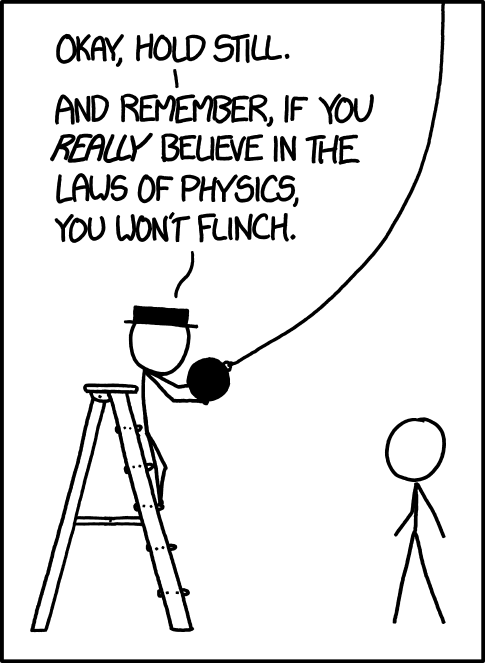
\includegraphics[height=8cm]{bilder/laws_of_physics_2x.png}
\end{figure}


%%%%%%%%%%%%%%%%%%%%%%%%%%%%%%%%%%%%%%%%%%%%%%%%%%%%%%%%%%%%%%%%%%%%%%%%%%%%%
\chapter{Vorkurs}
% !TEX ROOT = ../ersti.tex
\section{Vorkurs Mathematik}
Der Vorkurs für die Studienanfängerinnen der Mathematik und Informatik wird von der Fachschaft MathPhysInfo organisiert. Er soll helfen, euch den Einstieg in das Studium zu erleichtern und eine Einführung in die universitäre Mathematik geben. Dazu gibt es vormittags fachliche Vorträge und Übungen und nachmittags alles, was nicht direkt mit Mathe zu tun hat: wichtige Infos zum Studienalltag und ein umfangreiches Kennenlern- und Spaßprogramm. Den Vorkursplan mit Details zu Orten und Zeiten findet ihr im Internet\footnote{\label{mathe-vorkursplan}\url{https://mathphys.info/vorkurs/plan\#mathe}}. Die Woche beginnt am Montag, den 30. September mit der Begrüßungsveranstaltung um 9 Uhr im \gls{Mathematikon}.

% !TEX ROOT = ../ersti.tex
\section{Vorkurs Informatik}
Da im Informatikstudium in den ersten drei Semestern verhältnismäßig viele Mathe-Module belegt werden, ist der Mathe-Vorkurs auch für alle zukünftigen Infostudentinnen zu empfehlen. Es wird darüber hinaus eine Vorlesung zum Thema Algorithmen und Datenstrukturen geben, die auch für Mathestudentinnen interessant ist. Den Veranstaltungsplan (identisch mit dem Mathe-Vorkurs) findet ihr online\footnote{\label{info-vorkursplan}\url{https://mathphys.info/vorkurs/plan\#info}}.

\subsection{Programmiervorkurs}
Der Programmiervorkurs richtet sich an alle, die noch keinerlei Programmiererfahrung haben und vermittelt Grundlagen wie die Arbeit mit der Shell, Variablen, Schleifen, Funktionen, Objektorientierung in C++ und vieles mehr. Der Kurs findet vom 23. bis 27. September im \gls{Mathematikon} statt und ist auch für Mathematikerinnen zu empfehlen.

Die Kenntnisse werden in der \vl{Einführung in die praktische Informatik} (\gls{IPI}, erstes Semester) bzw. spätestens in der \vl{Einführung in die Numerik} (\gls{Num0}) hilfreich sein. Davon abgesehen ist es nützlich, erste Erfahrungen mit UNIX-artigen Betriebssystemen („Linux“) zu machen, da sie im naturwissenschaftlichen Bereich weit verbreitet sind.

Für den Programmiervorkurs ist aufgrund der begrenzten Plätze im Computer-Pool eine vorherige Anmeldung erforderlich! Den Link findet ihr ebenso im Vorkursplan.\footref{info-vorkursplan}

% !TEX ROOT = ../ersti.tex
\section{Vorkurs Physik}
Der Vorkurs Physik besteht aus einem mathematischen Vorkurs der Fakultät für Physik und Astronomie, gelesen von \dozentvorkurs. Dieser gehört zum Curriculum, ist aber nicht verpflichtend. Dennoch: ihr könnt hier bereits durch den Vorkurs eure ersten Credit-Points erhalten! Er beginnt am 23. September um 9 Uhr und findet vor Ort (INF 308, Hörsäle Physik) statt. Die genauen Inhalte des Vorkurses legen die Dozenten je nach Kenntnisstand der Hörerschaft fest, wobei das zugehörige Skript\footnote{\url{https://www.thphys.uni-heidelberg.de/~hefft/vk3/}} einen guten Anhaltspunkt bietet. Einen genauen Plan der Vorkursveranstaltungen und Orte findet ihr im Internet\footnote{\label{physik-vorkursplan}\url{https://mathphys.info/vorkurs/plan\#physik}}. Neben dem mathematischen Teil gehört zum Vorkurs Physik (ebenso wie zu den Mathe- und Info-Vorkursen) auch ein Wochenend- und Abendprogramm, organisiert von der MathPhysInfo.

% Den Vorkurs gibt es inzwischen auch als gebundenes Buch (siehe Buchliste). Geht ruhig mal in der ersten Vorkurswoche in die Universitätsbibliothek und leiht es euch sozusagen als Begleitbuch aus. (Vom Kauf möchten wir dennoch abraten.)

\begin{figure*}[!b]
    \centering
    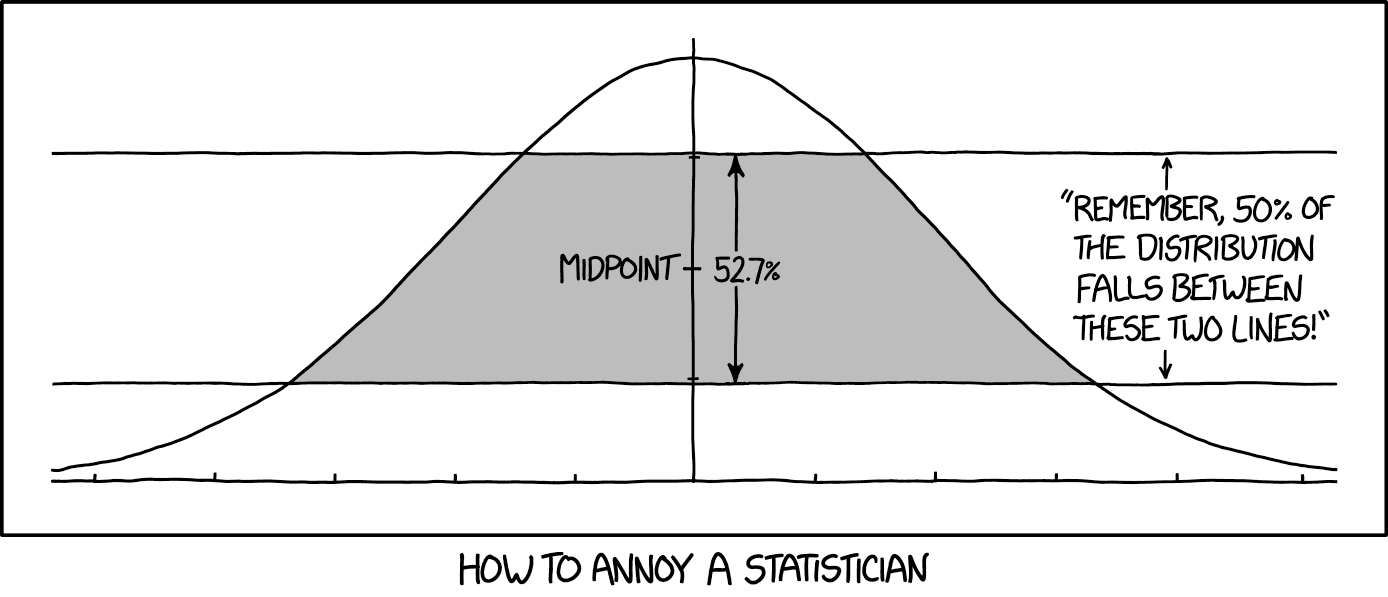
\includegraphics[width=\textwidth]{bilder/normal_distribution_2x.png}
    \caption*{It's the NORMAL distribution, not the TANGENT distribution.}
\end{figure*}

% !TEX ROOT = ../ersti.tex
\section{Rahmenprogramm}
\label{vorkurs-rahmenprogramm}

\subsection{Wanderungen}
An den Wochenenden -- Sonntag 09.10. und Sonntag 16.10. -- haben wir vor jeweils eine kleine Wanderung unternehmen. Die erste Tour führt auf den Heiligenberg, die zweite auf den Königstuhl -- die beiden Hausberge (Hügel) Heidelbergs. Im Anschluss an die erste Tour werden wir an der Thingstätte\footnote{alle Infos hierzu während der Wanderung erfragen} grillen, im Anschluss an die zweite Tour im Schlossgarten picknicken. Bringt euch für das Picknick alles Wichtige selbst mit.\\

Zusätzlich bieten wir am 29.09 eine spezielle Nachtwanderung an, die um 20 Uhr beginnt.

\noindent\emph{In der Regel treffen wir uns jeweils um 11 Uhr am Bismarckplatz. Coronabedingt kann es zu Änderungen kommen, die wir euch dann mitteilen.}

\vfill


\eject

\subsection{Spieleabende}
Das Abendprogramm wird spontan entschieden, meist handelt es sich um Gesellschaftsspiele -- bringt auf jeden Fall eigene Spiele mit, was auch immer ihr unter Spielen versteht.

Bisher sind Gesellschaftsspiele super angekommen -- da lernt man sich kennen -- Alternativvorschläge sind natürlich trotzdem immer gern gesehen. Falls euch etwas einfällt, meldet euch doch einfach, schließlich wird der Abend ja für euch veranstaltet.

Auch hier kann es zu Änderungen kommen, wir versuchen euch, eine digitale Möglichkeit anzubieten. Nähere Infos kommen noch.

\subsection{Brunch}
Am Samstag den 08. Oktober bereiten wir euch einen wunderschönen, leckeren Brunch im \gls{Mathematikon}, der das beste Frühstück wird, das ihr in euren ersten zwei Wochen bekommen werdet. Bringt bitte euer eigenes Geschirr/Besteck mit, damit wir Plastikquatsch sparen.


\vspace{4cm}

\begin{figure}[h]
\centering
\includegraphics[width=.7\linewidth]{bilder/su_doku.png}
\end{figure}


%%%%%%%%%%%%%%%%%%%%%%%%%%%%%%%%%%%%%%%%%%%%%%%%%%%%%%%%%%%%%%%%%%%%%%%%%%%%%
\chapter{Studiengänge}
\section{Bachelor Allgemein}
In den ersten Semestern besuchen die meisten Studis die sog. \emph{Pflichtvorlesungen}. Gerade die ersten beiden Semester sind i.d.R. mit diesen Grundvorlesungen gut gefüllt. Ab dem dritten Semester belegen dann viele die ersten \emph{Wahlpflichtveranstaltungen}, bei denen du für bestimmte Module (s.u.) aus mehreren Lehrveranstaltungen die wählst, die dir am ehesten zusagen. Im Bachelor gibt es vier Bereiche: \emph{Pflicht-}, \emph{Wahlpflicht-} und der Bereich \emph{Fachübergreifende Kompetenzen (FüK)}, sowie den \emph{Wahlbereich} (Physik) bzw.~ein \emph{Anwendungsgebiet} (Mathe/Info).

\begin{itemize}
	\item Pflichtbereich: Grundlagen des Studienfachs und fachliche Methodik
	\item Wahlpflichtbereich: Spezialisierung auf einem Gebiet
	\item FüK: Soft Skills und fachübergreifendes Wissen
	\item Anwendungsgebiet: Interdisziplinäre Anwendung eures Fachwissens
\end{itemize}

\paragraph*{Module} sind \glqq{}thematisch und zeitlich abgeschlossene Lehr- und Lerneinheiten\grqq{}, in die euer Studium gegliedert ist. Verständlich: Das sind

\begin{itemize}
	\item Vorlesungen, meist mit einer Klausur am Ende,
	\item Seminare, in denen eure Prüfung aus einem Vortrag und einer schriftlichen Ausarbeitung besteht,
	\item Praktika, in denen ihr lernt, euer Wissen anzuwenden.
\end{itemize}

Teilweise bestehen Module aus mehreren Veranstaltungen. Dann müsst ihr zum Abschließen des Moduls nicht nur \textit{eine} Prüfung bestehen oder einen Vortrag halten, sondern \textit{alle}\footnote{rechtlich heißt es zwar „ein Modul, eine Prüfung“, aber man kann da Ausnahmen machen} Veranstaltungen des Moduls bestehen.

Zur Vertiefung und Übung der Themen gibt es in fast allen Vorlesungen jede Woche einen Übungszettel mit Aufgaben zum aktuellen Thema. Dabei wiederholt und übt man den Vorlesungsstoff und erarbeitet sich die notwendigen Punkte für die Klausurzulassung (i.d.R. reichen 50\% aller Punkte). Das jeweilige System wird euch immer am Anfang des Semesters in jeder Vorlesung erklärt.

Für bestandene Module bekommt ihr dann \gls{LP}\footnote{manchmal auch \gls{CP} genannt}, von denen ihr in eurem Studium insgesamt 180 sammeln müsst (mit einigen Bedingungen verknüpft), um euren Bachelor zu bekommen. Die Anzahl der Punkte pro Modul errechnet sich aus einem von den Dozierenden jeweils festgelegten Schlüssel, der die benötigte Zeit für den Besuch der Vorlesung, die Übungsaufgaben und das Selbstlernen mit Vor- und Nachbereitung der Vorlesungen widerspiegeln soll. Ein \gls{LP} entspricht etwa 30 Stunden Arbeit im Semester, also gute zwei Stunden pro Woche. Da es natürlich stark von euch abhängt, wie lange ihr für das alles braucht und wie viel Zeit ihr wirklich investieren wollt, kann das nur eine grobe Abschätzung sein, ist aber eine gute Orientierung, wenn ihr überlegt, wie viel ihr euch im Semester aufbürden wollt.

Genaue Informationen zu den Modulen, Modellstudienplänen und die Prüfungsmodalitäten findet ihr auf den Seiten der Uni\footnote{\url{https://uni-heidelberg.de/studium/download/stud_pruef.html}} in eurem jeweiligen Modulhandbuch bzw. eurer Prüfungsordnung. Bei Unklarheiten geben euch eure Prüfungssekretariate rechtsverbindliche Auskünfte und beantworten Fragen zur Prüfungsordnung. 
\begin{itemize}
	\item Physik: \pruefsekphysik
	\item Mathe: \pruefsekmathe
	\item Info: \pruefsekinfo
\end{itemize}

% !TEX ROOT = ../ersti.tex
\section{Informatik 100\%}

\begin{figure}[b]
    \centering
    \includegraphics[height=5cm]{bilder/ambition.png}
\end{figure}

\begin{figure*}[th]
    \centering
    \begin{subfigure}{.23\textwidth}
        \includegraphics[height=5cm]{bilder/backing_up_1.png}
    \end{subfigure}
    \begin{subfigure}{.23\textwidth}
        \includegraphics[height=5cm]{bilder/backing_up_2.png}
    \end{subfigure}
    \begin{subfigure}{.23\textwidth}
        \includegraphics[height=5cm]{bilder/backing_up_3.png}
    \end{subfigure}
    \begin{subfigure}{.23\textwidth}
        \includegraphics[height=5cm]{bilder/backing_up_4.png}
    \end{subfigure}
\end{figure*}

\subsection{Die ersten Semester}

Im ersten Semester hört ihr nach Studienverlaufsplan (s. Modulhandbuch) die \vl{Einführung in die Praktische Informatik} (\gls{IPI}), \vl{Einführung in die Technische Informatik} (\gls{ITE}), den \vl{Programmierkurs} (\gls{IPK}) und eine Mathematikvorlesung. Die \gls{IPI} vermittelt Grundkenntnisse und -konzepte der Informatik anhand mindestens einer Programmiersprache. Im \gls{IPK} vertieft ihr eure Programmierkenntnisse und in \gls{ITE} lernt ihr Grundlegendes über Rechnerarchitektur und die dazugehörigen logischen Schaltungen. Aufgepasst! Die \gls{IPI} ist in der Informatik eure einzige \emph{Orientierungsprüfung} und ihr müsst sie bis zum Ende des dritten Semesters bestanden haben.


\subsection{Später dann \dots{}}

\dots{} werden einzelne Themengebiete eröffnet und vertieft. Die Namen der Vorlesungen sprechen zum größten Teil für sich, zum Beispiel \vl{Datenbanken} (\gls{IDB1}) oder \vl{Betriebssysteme und Netzwerke} (\gls{BeNe} bzw. IBN). Außerdem besucht ihr ein \vl{Bachelorseminar} sowie ein \vl{An\-fän\-ger--} und ein \vl{Fortgeschrittenen--Praktikum} (\gls{AP} und \gls{FP}). Diese unterscheiden sich von Vorlesungen, da von der Modulbeschreibung kein inhaltliches Thema vorgegeben wird, sondern lediglich die Veranstaltungsform.

\paragraph*{Im Bachelorseminar} erklärt ihr jeweils den anderen Studis in einem Vortrag ein euch zuvor zugeteiltes Thema aus einem zusammenhängenden Themenbereich und schreibt eine Ausarbeitung dazu. Was die tatsächliche Schwerpunktsetzung eures Vortrags und Ausarbeitung ist, variiert aber von Dozentin zu Dozentin und wird euch jeweils am Anfang erklärt und im Währenden betreut.

\paragraph*{Praktika} sind i.d.R. Projekte mit einigermaßen freier Zeiteinteilung, die am Ende des Semesters fertig sein müssen und in Gruppen bearbeitet werden. Die Praktika wechseln von Zeit zu Zeit, es gibt aber üblicherweise jedes Jahr Angebote in Bereichen wie Technische Informatik und Software Engineering.

\subsection{Mathe und so \dots}

Informatikstudium in Heidelberg heißt, ihr hört vergleichsweise viel Mathe. Dabei habt ihr die Wahl zwischen mehreren Varianten, in der Hauptsache gibt es aber diese beiden Wege, bei denen ihr die für euer weiteres Studium relevanten Grundkenntnisse vermittelt bekommen sollt:

\begin{itemize}
    \item Mathe bei den Mathematikerinnen, also \vl{Lineare Algebra 1} (\gls{LA}) und \vl{Analysis 1} (\gls{Ana}). \gls{LA} und \gls{Ana} können entweder beide im ersten oder \gls{LA} im ersten und \gls{Ana} im dritten Semester gehört werden.
    \item \vl{Mathematik für Informatiker 1} (\gls{MafIn} bzw. IMI, entspricht etwa \gls{LA} 1) im ersten und \vl{Mathematik für Informatiker 2} (ersetzt \gls{Ana} 1) im zweiten Semester. Weiteres dazu im \autoref{mafin}.
\end{itemize}

Danach hört ihr im Modul \vl{Mathematische Grundlagen 3} eines der drei Module \vl{Einführung in die Numerik} (\gls{Num0}), \vl{Einführung in die Wahrscheinlichkeitstheorie und Statistik} (\gls{WTheo0}) oder \vl{Analysis 2} (\gls{Ana2}). Die Mathematikmodule unterscheiden sich stark von der Schulmathematik. Unterschätzt den Aufwand für die Vorlesungen nicht! Wollt ihr euer Informatikstudium mathematisch ausrichten (z.B. Richtung Wissenschaftliches Rechnen oder Machine Learning), empfehlen wir, die Mathevorlesungen \gls{LA} und \gls{Ana} bei den Mathematikerinnen zu hören.

\subsection{Programmieren. Und dann \dots}

Programmieren ist eine wichtige Fertigkeit, die ihr außerhalb von \gls{IPI} und \gls{IPK} hauptsächlich im Selbststudium erlernen oder vertiefen werdet. Solide Kenntnisse von unixoiden Systemen, wie Linux und OSX, sind immer Gold wert. Im Informatikstudium wird \emph{fast ausschließlich mit Linux} gearbeitet. Die Uni hilft aber auch noch ein bisschen: Neben den Pflichtkursen \gls{IPI} und \gls{IPK} gibt es in der \gls{Num0} praktische Übungen, in denen ebenfalls programmiert wird. Eigeninitiative ist aber dennoch wichtig und mit interessanten Projekten macht das Lernen auch enorm viel Spaß.

\subsection{Anwendungsgebiet}

Neben der wunderbaren Welt der Informatik sollt ihr euch aber auch mit deren Anwendungsgebieten auseinandersetzen. Dazu müsst ihr 24 \gls{LP} in mindestens einem anderen Fach erreichen. Entgegen der häufigen Vermutung hört ihr hier also einfach fachfremde Vorlesungen, um euren Horizont interdisziplinär zu erweitern, in denen ihr weder programmiert, noch sonstige Informatikkenntnisse vermittelt bekommt. Obwohl nur wenige Fächer im Modulhandbuch als Anwendungsgebiete vorgeschlagen werden, könnt ihr nach \emph{vorheriger} schriftlicher Bestätigung eures Prüfungssekretariats auch andere Fächer wählen, die euch interessieren. Dabei sind die Module von den Fachbereichen normalerweise fest vorgeschrieben, Nachfragen im Prüfungssekretariat des Anwendungsgebiets lohnt sich aber, da es manchmal doch einige Wahlmöglichkeiten gibt. Insbesondere ist zu beachten, dass Veranstaltungen nicht unbedingt in jedem Semester angeboten werden, das Anmeldeprozedere sich von dem in der Informatik unterscheidet und teilweise sogar andere e-Learningplattformen und Vorlesungsorte genutzt werden.

\subsection{Orientierungsprüfung}

Die \vl{Einführung in die Praktische Informatik} \emph{müsst} ihr, als eure Orientierungsprüfung, bis zum Ende des dritten Semesters bestanden haben.


\subsection{Prüfungen: wie und wieso?}

Um in den Vorlesungen \gls{LP} zu erhalten und somit das Modul abzuschließen, müsst ihr fast immer eine Klausur am Semesterende bestehen. Über die genauen Prüfungsmodalitäten informieren euch eure Dozierenden jeweils am Anfang des Semesters. Meist müsst ihr für die Klausurzulassung eine Mindestpunktzahl (i.d.R. 50\%) aus den Übungszetteln erreichen.

Häufig habt ihr pro Modul zwei Versuche, es ist also noch kein Beinbruch, wenn ihr beim ersten Versuch nicht bestanden habt. Die konkreten Regelungen sind aber zwischen den jeweiligen Modulgruppen etwas verschieden, informiert euch also am \emph{Anfang des Semesters} immer genau über die Bedingungen! Solltet ihr eine Prüfung auch beim letzten Versuch nicht bestehen, so besteht in bis zu drei Fällen die Möglichkeit, die Prüfung \emph{auf Antrag beim Prüfungsausschuss} ein weiteres Mal zu wiederholen (gilt nicht für Orientierungsprüfung und Bachelorarbeit). Besteht ihr auch diesen Versuch nicht, verliert ihr euren Prüfungsanspruch endgültig und werdet somit exmatrikuliert. Dies und weitere studienrelevante Vorschriften sind in der Prüfungsordnung geregelt, deshalb lohnt es sich definitiv, die Prüfungsordnung einmal komplett zu lesen. Außerdem kann sich diese leider immer mal wieder ändern, darauf sollte man achten.

\emph{Klausuranmeldungen sind immer verbindlich}. Überlegt euch also gut, ob ihr euch anmeldet. Solltet ihr euch sicher sein, die Klausur nicht zu bestehen, empfiehlt es sich, sich nicht direkt für diesen Versuch anzumelden, sondern erst die zweite Klausur wahrzunehmen oder zur Not die Vorlesung im nächsten Jahr noch einmal zu hören. Eure Klausurzulassung ist ein Jahr lang gültig. Das Schöne an eurem Studiengang ist, dass ihr zwei Noten streichen könnt, die dann nicht in eure Abschlussnote zählen. Das heißt, auch wenn eine Prüfung mal nicht so gut läuft, muss eure Abschlussnote darunter nicht unbedingt leiden.

\begin{figure}[t]
    \centering
    \includegraphics[width=.6\linewidth]{bilder/haskell.png}
\end{figure}

\begin{figure*}[b]

    \begin{subfigure}{.23\textwidth}
        \includegraphics[height=5cm]{bilder/cant_sleep_1.png}
    \end{subfigure}
    \hfill
    \begin{subfigure}{.23\textwidth}
        \includegraphics[height=5cm]{bilder/cant_sleep_2.png}
    \end{subfigure}
    \hfill
    \begin{subfigure}{.23\textwidth}
        \includegraphics[height=5cm]{bilder/cant_sleep_3.png}
    \end{subfigure}
    \hfill
    \begin{subfigure}{.23\textwidth}
        \includegraphics[height=5cm]{bilder/cant_sleep_4.png}
    \end{subfigure}

\end{figure*}

%\vspace{-\parskip}

\section{Mathematik 100\%}

\subsection{Das erste und zweite Semester}

In den ersten zwei oder drei Semestern hört ihr eure Grundvorlesungen und einige Einführungsvorlesungen. Die Grundvorlesungen sind die \vl{Lineare Algebra 1} und \vl{2} (\gls{LA}), in denen ihr hauptsächlich Abbildungen zwischen Vektorräumen betrachtet, und \vl{Analysis 1} und \vl{2}, sowie \vl{Höhere Analysis} (\gls{Ana}). Dort behandelt ihr Grenzwerte mit allem, was folgt, das heißt Differential- und Integralrechnung.

In den Anlagen der Prüfungsordnung findet ihr nochmal eine Auflistung, wie euer Studium aufgebaut ist. Auch das sind nur Vorschläge; wie ihr euer Studium im Endeffekt einteilt bleibt natürlich euch überlassen.

\subsubsection{Orientierungsprüfungen}

Orientierungsprüfungen sind Prüfungen, die bis Ende des dritten Semesters bestanden sein müssen, da man ansonsten exmatrikuliert wird und den Prüfungsanspruch für das jeweilige Fach in ganz Deutschland verliert. In der Mathe sind das \gls{Ana}~1 und \gls{LA}~1 für den 100\%-Bachelor, bzw. \gls{LA}~1 für 50\%-Bachelor. Es ist daher sinnvoll, diese Vorlesungen im ersten Semester zu hören. Sollte man im ersten Anlauf, das heißt in der ersten Klausur und in der Nachklausur, nicht bestehen, ist das noch lange kein Weltuntergang. Ihr seid damit nicht die Ersten und nicht die Letzten an der Uni und sicher auch nicht die Einzigen in eurem Semester. Es fallen in manchen Jahren 50\%, mal mehr, mal weniger, durch diese Klausuren durch. Macht euch deshalb also keinen Kopf! Ihr habt dann im Wintersemester darauf noch einen Versuch, bestehend aus Klausur und Nachklausur. Der muss dann aber klappen, da euch sonst die Exmatrikulation droht.

\subsubsection{Einführungsvorlesungen}

Die Einführungsvorlesungen bestehen aus der \vl{Einführung in die praktische Informatik} (\gls{IPI}), \vl{Einführung in die Numerik} (\gls{Num0}) und \vl{Einführung in die Wahrscheinlichkeitstheorie und Statistik} (\gls{WTheo0}). In allen Vorlesungen löst ihr Übungszettel, die dazu dienen, den Stoff zu vertiefen. Ihr habt dann zu jeder Vorlesung Übungsgruppen und Tutorinnen, die nicht nur eure Zettel korrigieren und sie mit euch besprechen, sondern vor allem dazu da sind, euch zu helfen. Tutorinnen werden dafür bezahlt, eure Fragen zu beantworten, egal wie dumm diese euch in dem Moment vorkommen, und machen das auch gerne. Auch die anderen Studis verstehen meist nicht mehr als ihr, sehr wahrscheinlich haben sie ähnliche Fragen. Sucht euch am besten am Anfang eine Gruppe von Kommilitoninnen, mit denen ihr gut rechnen und überlegen könnt, damit ihr die Zettel nicht alleine bearbeiten müsst. Abgeben sollt ihr sie auch nicht alleine, sondern im Allgemeinen zu zweit.

Zusätzlich kann im zweiten Semester ein Proseminar besucht werden. Das Proseminar setzt eine aktive Teilnahme voraus und wird mit einem mündlichen Vortrag abgeschlossen, eventuell mit zusätzlicher schriftlicher Ausarbeitung. Der Vortrag ist eine sehr gute Möglichkeit \LaTeX\ zu lernen. \LaTeX\ ist ein Programm, um PDF-Dokumente zu schreiben. Ihr werdet es in eurem Mathestudium noch häufig brauchen. Und wie heißt es so schön: Früh übt sich, wer ein Meister werden will \textit{(Schiller)}.

\subsubsection{Ist Mathe wirklich richtig für mich?}

In den ersten beiden Semestern kann es passieren, dass eure Noten nicht so gut sind, wie ihr das vielleicht gerne hättet oder gewohnt seid. Das ist aber noch lange kein Weltuntergang und auch kein Grund, das Studium abzubrechen, wenn ihr Spaß an Mathematik habt. Mathematik an der Uni ist etwas ganz anderes als die Mathematik, die man aus der Schule kennt. Es wird auch gerne die Tatsache unterschätzt, dass man plötzlich in einer ganz neuen Situation ist: einer für die meisten fremde Stadt mit neuen Leuten und in einem ganz anderen System als der Schule. Man muss sich erst einmal an die geänderten äußeren Umstände gewöhnen und das braucht Zeit. Auch die Klausuren sind nicht so schlimm, wie es einem am Anfang vorkommen mag. Ihr habt im Regelfall eine zweite Chance, wenn ihr durch die erste durchfallt. Sollte auch der zweite Anlauf nicht klappen, dann könnt ihr die Vorlesung im nächsten Jahr noch einmal hören. Es ist also nichts verloren. Verzweifelt nicht zu schnell an der noch sehr ungewohnten Uni-Mathe, ihr werdet euch schnell daran gewöhnen. Ebenfalls wird aus \gls{LA} 1 und 2 sowie \gls{Ana} 1 und 2 auch nur die jeweils bessere Lineare-Algebra- und Analysis-Note in eurem Bachelor berücksichtigt.

Wenn ihr sonst über irgendetwas stolpert, gibt es immer noch die Fachschaft, die euch gerne weiterhilft. Ihr könnt entweder persönlich bei uns vorbei kommen oder eine \href{mailto:fachschaft@mathphys.info}{Mail} schreiben. Wir versuchen dann, euch zu helfen, wo es nur geht.

\subsection{Alle weiteren Semester}

Der weitere Verlauf des Studiums kann von jeder Studentin ganz individuell gestaltet werden. Man kann sich dabei nach einem der Stundenpläne, die auf der Homepage der Fakultät zu finden sind, richten. Bei der Frage, welche Vorlesungen und Veranstaltungen ihr belegen müsst und könnt, helfen euch Modulhandbuch, Prüfungsordnung und die Webseite der Fakultät.

\subsection{Prüfungsordnung}

In der Prüfungsordnung (\gls{PO}) findet ihr alle wichtigen Informationen darüber, welche Veranstaltungen gehört werden müssen, welche Prüfungen wann und wie abgelegt werden müssen und wie euer Studium sonst geregelt ist. Außerdem könnt ihr dort nachschlagen, welche Pflicht- und Wahlpflichtveranstaltungen es gibt und wie viele und welche gehört werden müssen (Anlage 1 und 2).  Im Modulhandbuch findet ihr kurze Beschreibungen der Veranstaltungen und welche Vorkenntnisse für sie empfohlen werden. Neben Pflicht- und Wahlpflichtmodulen gibt es noch das Anwendungsgebiet und fachübergreifende Kompetenzen. Über letztere braucht ihr euch keine großen Sorgen zu machen, die hat man meist schneller als man denkt. Möglichkeiten sind hier Praktika, Auslandssemester, Sprachkurse, die das Zentrale Sprachlabor der Universität Heidelberg anbietet, Vorlesungen anderer Fächer und so weiter. 8 der 20 Leistungspunkte für fachübergreifende Kompetenzen sind bereits in andere Veranstaltungen integriert. In Anlage 3 der PO findet ihr mehr Informationen darüber, wie und wann ihr diese Leistungspunkte erwerbt. Es lohnt sich definitiv, die Prüfungsordnung einmal komplett zu lesen. Außerdem kann sich diese leider immer mal wieder ändern, darauf sollte man achten.

\subsection{Anwendungsgebiet}

Zusätzlich zum puren Mathematik-Studium habt ihr das Anwendungsgebiet, was ein Fach eurer Wahl sein kann. In der Prüfungsordnung gibt es aber nur für die Fächer Informatik, Physik, Astronomie, Biologie, Chemie, Wirtschaftswissenschaften und Philosophie eine feste Regelung. Nach Rücksprache mit dem Prüfungsausschuss können jedoch auch andere Fächer angerechnet werden. Habt ihr zum Beispiel ein Studium vorher abgebrochen, kann das oft als Anwendungsgebiet angerechnet werden. Die meisten der oben genannten Fächer fangen laut Musterstudium in eurem dritten Semester an, die interessanten Informatikvorlesungen sind dagegen im Sommersemester. Niemand wird euch daran hindern, euer Anwendungsgebiet schon im ersten Semester zu beginnen, unterschätzt jedoch die Arbeitsbelastung des Grundstudiums nicht.

\subsection{Am Ende Bachelor?}

Ganz am Ende erwarten euch dann noch ein weiteres Seminar, welches häufig als Grundlage für die Bachelorarbeit verwendet wird, und zuletzt die Bachelorarbeit und das zugehörige Bachelorseminar, in dem ihr in der Regel die Arbeit präsentiert.

% !TEX ROOT = ../ersti.tex
\section{Physik 100\%}

\subsection{Erstes Semester}
Das erste Semester ist, verglichen mit späteren Semestern, sehr stark durchstrukturiert, was euch den Wechsel von der Schule an die Uni erleichtert, jedoch auch nicht besonders viele Freiheiten lässt.  Allgemein werdet ihr bis ins vierte Semester im Pflichtprogramm je eine \vl{Experimentalphysik} (\gls{Ex}) und eine \vl{Theoretische Physik} (\gls{Theo})\footnote{Die Abkürzung „Theo“ kann zu Verwirrungen mit Informatikerinnen führen, da diese das als \vl{Theoretische Informatik} verstehen.} Vorlesung besuchen, wobei im fünften Semester noch die \gls{Ex} 5 folgt. Zusätzlich dazu hört ihr im ersten Semester die \vl{Höhere Mathematik für Physiker 1} oder die \vl{Lineare Algebra 1} (\gls{LA}) und wenn ihr wollt auch die \vl{Analysis 1} (\gls{Ana}); aber zur Mathematik später mehr.

Das ganze Semester über werdet ihr in jeder Vorlesung wöchentlich einen Übungszettel bekommen, den ihr innerhalb einer Woche lösen sollt. Diese dienen zum Einüben des in den Vorlesungen behandelten Stoffes und zugleich häufig als Klausurzulassung (und gute Vorbereitung!). Man benötigt meist insgesamt 50 bis 70\% der Gesamtpunktzahl auf allen Zetteln, aber wenn es nur um ein paar Punkte geht, sind die Tutorinnen kulant. Wenn eure Tutorin den Eindruck hat, ihr verschwendet mit der Klausur keinen Prüfungsversuch, lässt sie euch meistens zu. Macht euch darum aber erstmal keinen Kopf, wenn ihr am Ball bleibt, ist das überhaupt kein Problem, ihr müsst die Zettel ja nicht alle alleine lösen.

\subsection{Orientierungsprüfung}
Die Orientierungsprüfung ist eine Prüfung, die ihr bis zum Ende des 3. Semesters bestehen müsst, um weiterhin Physik studieren zu dürfen. Im Bachelor Physik ist dies die ganz normale Klausur in der \gls{Ex} 1. Dort werden meist sehr schulnahe physikalische Grundlagen der Mechanik behandelt. Macht euch also keine Sorgen. Das schafft ihr!

\subsection{Basiskurs}
Der Basiskurs beginnt in der letzten Vorkurswoche und soll euch den Einstieg in das Studium erleichtern. Dabei werden euch sogenannte Schlüsselkompetenzen beigebracht, die unter anderem in Zeitmanagement, Literatursuche und das Textsatzsystem \LaTeX{} einführen. Auch wenn ihr vermutlich schon einiges davon kennt, ist es doch ganz nett, nochmal alles kompakt zu sehen und vor allem dabei neue Menschen und vielleicht auch spätere „Zettelpartnerinnen“ kennenlernen zu können. Die Qualität des Kurses ist naturgemäß stark abhängig von eurer Tutorin. Ihr müsst also für euch bestimmen, wie viel ihr aus diesem Kurs mitnehmt. Stellt auf jeden Fall viele Fragen.

\begin{figure}[b]
	\centering
	\includegraphics[width=\linewidth]{bilder/both_irrational.png}
\end{figure}


\subsection{Lineare Algebra und Analysis vs.~Höhere Mathematik für \\Physiker}
Ihr habt zwei Möglichkeiten, die für das Studium benötigte Matikmodule zu belegen.
In der ersten Variante hört ihr in den ersten drei Semestern die Vorlesungen \vl{Höhere Mathematik für Physiker} 1 bis 3. Alternativ könnt ihr die \vl{Lineare Algebra 1} im ersten Semester und dann die \gls{Ana} 2 und 3 hören. Falls ihr euch dafür entscheidet, empfiehlt es sich stark, zusätzlich im ersten Semester die Vorlesung \gls{Ana} 1 zu hören, da diese die fachliche Grundlage für \gls{Ana} 2 und \gls{Ana} 3 bietet. Trotzdem könnt ihr noch zum zweiten oder dritten Semester zwischen \gls{Ana} und \gls{HoMa} neu entscheiden. Mehr zu den einzelnen Vorlesungen, damit ihr euch am Ende auch entscheiden könnt auf \autopageref{mathephysik}.

\subsection{Weiteres Studium}

Euer weiteres Studium sieht, wie oben kurz angedeutet, so aus, dass ihr immer ein Grundgerüst an Vorlesungen habt und euch darum herum andere Vorlesungen und Seminare selbst auswählen könnt. Die Experimentalphysikvorlesungen sind bis zum fünften Semester und die theoretischen bis zum vierten Semester verpflichtend. Hinzu kommen in den ersten drei Semestern entweder die \gls{HoMa} 1 bis 3 oder die \gls{LA} 1 und die \gls{Ana} 2 und 3. Ansonsten seid ihr jedoch bis auf ein Pflichtseminar, das ihr aus einem relativ großen Topf an Seminaren auswählen könnt, und den Pflichtpraktika frei, alles zu hören, was euch so in den Sinn kommt. Ihr müsst einzig darauf achten, dass ihr in den einzelnen Bereichen ausreichend „Punkte sammelt“: Im Wahlpflichtbereich sind das 14 \gls{LP}, bei den Übergreifenden Kompetenzen 19 \gls{LP} und im Wahlbereich bis zu 17 \gls{LP}. Nutzt frühzeitig die Gelegenheit, Veranstaltungen zu besuchen, die euch interessieren, dann macht das Studium gleich doppelt so viel Spaß!

\begin{figure}[b]
	\centering
	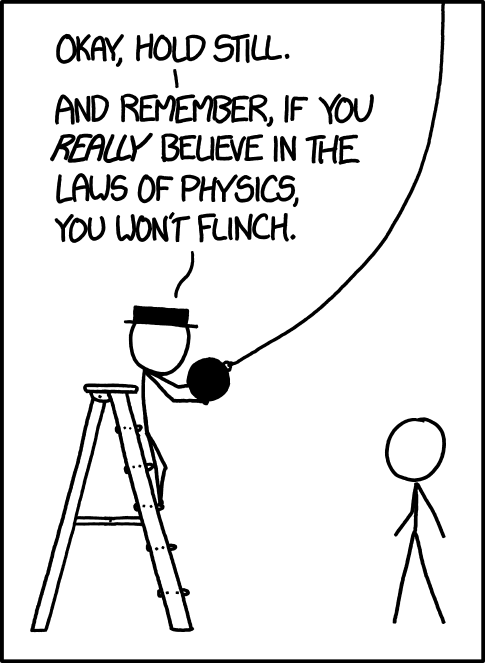
\includegraphics[width=.85\linewidth]{bilder/laws_of_physics_2x.png}
\end{figure}
\vfill \eject

\subsection{Wahlbereich, Wahlpflichtbereich und \\Übergreifende Kompetenzen}

Im Laufe eures Bachelorstudiums müsst ihr ggf. ein oder zwei Wahlfächer belegen, welche ihr aus einem recht weit gefächerten Angebot wählen könnt. Diese Wahlfächer müssen auch nicht aus Bereichen der Physik kommen, sondern können z.B. Mathe, Chemie oder Philosophie sein. Was ihr alles für Möglichkeiten habt, könnt ihr genauer in der Prüfungsordnung nachlesen und selbst Fächer, die dort nicht aufgezählt sind, lassen sich möglicherweise nach Absprache mit dem Prüfungsausschuss auch anrechnen.

Der Wahlpflichtbereich besteht, im Gegensatz zum Wahlbereich und den Übergreifenden Kompetenzen, aus vertiefenden oder weiterführenden Physikveranstaltungen. Schaut doch einfach in das Vorlesungsverzeichnis im HeiCO und sucht euch interessante Vorlesungen oder auch Seminare aus. Besonders Seminare können viel Spaß machen, da diese zwar oftmals viel selbstständiges Arbeiten verlangen, aber auch forschungsnäher sind als Vorlesungen. Zudem findet ihr Anregungen dazu in der Prüfungsordnung und im Modulhandbuch.

Der Bereich Übergreifende Kompetenzen soll euch ein wenig dazu bewegen, fachunabhängige Kompetenzen zu erlernen. Darunter fallen der mathematische Vorkurs, der Basiskurs, sowie alle als „Überfachliche Kompetenzen“ gekennzeichneten Module der Mathematik, Informatik und den Naturwissenschaften. Außerdem lassen sich oft nach Rücksprache mit dem Prüfungssekretariat auch weitere Veranstaltungen anrechnen, wie zum Beispiel Sprachkurse, Programmierkurse, usw.

Allgemein gilt: versucht möglichst früh Dinge aus Gebieten zu hören, die euch interessieren; denn das sind die Fächer die euch auch wirklich Spaß machen und ihr erlangt ein möglichst breites, und vor allem tiefes Wissen, welches euch bei eurer Bachelorarbeit und vermutlich auch sonst zugutekommt.

\subsection{Prüfungen und Noten}

Es wird euch sicher freuen zu hören, dass eine nicht bestandene Klausur nicht gleich das Ende für euer Studium bedeutet. Im Grunde ist die Wiederholungsregelung sogar recht studifreundlich; so habt ihr in jedem Modul zwei Versuche, wobei in der Regel ein Versuch aus einer Klausur und, wenn nötig, der dazugehörenden Nachklausur besteht. Darüber hinaus habt ihr für euer Studium noch zwei sogenannte Joker, die euch jeweils einen dritten Versuch geben, falls die zwei regulären nicht reichen sollen (dies gilt nicht für eure Orientierungsprüfung, welche die Prüfung in der \gls{Ex} 1 darstellt). Darüber hinaus ist für euch recht interessant, dass es die Möglichkeit gibt, zwei Noten aus unterschiedlichen Bereichen der tendenziell schlechteren Pflichtmodule zu streichen. Macht euch also nicht zu viele Gedanken darüber, wenn eure Noten zunächst nicht ganz so gut sind. Auch könnt ihr jederzeit zusätzlich gehörte Module in den Bereich der Zusatzleistungen verschieben, wenn ihr diese nicht benötigt, euch entsteht also kein Nachteil dadurch, dass ihr mehr hört, als ihr müsst.

Sonst ist noch zu erwähnen, dass ihr, um in Heidelberg in den Master zugelassen zu werden, eine Bachelornote von 2,9 oder besser braucht. Das war bislang noch nie ein Problem für Heidelberger Studis, der Notenschnitt liegt zwischen 1,7 und 2,0.

\subsection{Regel- und Maximalstudienzeit}

Vielleicht ist euch das ominöse Wort \emph{Regelstudienzeit} vor eurem Studium bereits zu Ohren gekommen. An dieser Stelle wollen wir mit ein paar Mythen, die sich um sie ranken, aufräumen.

Obwohl das Wort es suggeriert, ist es keinesfalls die Regel, dass Studierende ihr Studium in Regelstudienzeit abschließen. Es handelt sich also nicht um die durchschnittliche Studiendauer, welche je nach Fach mehr oder weniger deutlich über den vorgesehenen sechs Semestern für den Bachelor und vier für den Master liegen. Die Regelstudienzeit gibt lediglich an, wie schnell man ein Studium abschließen kann, wenn man jedes Semester im Schnitt 30 Leistungspunkte absolviert. Die Fakultäten gehen dabei die Selbstverpflichtung ein, dass ein Studium in der Regelstudienzeit studierbar ist.

Die Gründe für ein längeres Studium sind vielfältig, neben Lohnarbeit zur Finanzierung des Studiums oder nicht bestandenen Prüfungen sind diese auch nicht alle negativ konnotiert. So hören viele Studierende aus Interesse zusätzliche Vorlesungen, bevor sie ihre Abschlussarbeit abschließen. Intensives ehrenamtliches Engagement, z.\,B.~in der Hochschulpolitik kann ebenfalls ein Grund sein. Ebenfalls ist es üblich, dass ein Auslandsaufenthalt im Studium zu einer Verlängerung des Studiums führt.

Wie ihr seht, ist es also ein weit verbreiteter Irrglaube, dass nur faule oder schlechte Studentinnen länger als vorgesehen studieren würden. Die Universität ist nun mal kein Ausbildungsbetrieb im klassischen Sinne, sondern dient neben dem Erwerb fachlicher Kompetenzen auch dem Entwickeln der Persönlichkeit und dem interdisziplinären Wissenserwerb. Sie bietet eine unvergleichliche Lernumgebung, auf die man, einmal im Arbeitsleben angelangt, mit Sehnsucht zurückschaut. Die Mentalität, die wir euch ans Herz legen wollen, ist, dass ihr euch nicht unter Druck setzen lasst und das Studium in der euch angemessen erscheinenden Zeit absolviert.

Es gibt jedoch zwei Wermutstropfen. Der BAföG-Anspruch ist auf das Studium in Regelstudienzeit beschränkt; es gibt aber viele Möglichkeiten, bis zu zwei Semester pro Studienabschnitt länger BAföG zu beziehen. Ebenfalls sei angemerkt, dass die Physik in ihrer Prüfungsordnung verankert hat, dass man die letzte Prüfungsleistung spätestens im dritten Semester nach Überschreiten der Regelstudienzeit absolvieren muss, was einer Maximalstudiendauer von neun Semestern im Bachelor entspricht. Wenn man diese überschreitet, müsste man also formal exmatrikuliert werden, in der Realität wird dies jedoch nach unserem Stand der Dinge nie durchgezogen. Die Fakultät hat kein Interesse daran, Personen, die in ihrem zehnten Semester kurz vor dem Abschluss stehen, zu exmatrikulieren. Diese Grenze wird viel mehr als eine notwendige extrinsische Motivation angesehen, zielstrebig zu studieren. Macht euch deswegen also keinen Kopf!

\subsection{Prüfungsordnung und Modulhandbuch}

\begin{figure*}[b]
	\centering{
		\includegraphics[width=\textwidth]{bilder/purity.png}
	}
\end{figure*}

Immer dann, wenn sich euch Fragen zu eurem Studium stellen oder ihr euch einfach über den weiteren Studienverlauf informieren wollt, sind die ersten Anlaufstellen die Prüfungsordnung und das Modulhandbuch. In der Prüfungsordnung ist formal geregelt, wie der Studienablauf, die Prüfungen und die Anrechenbarkeit von Modulen aussehen. Das Modulhandbuch wiederum ist im Großen und Ganzen eine Auflistung der in der Physik (und benachbarten Gebieten) angebotenen Veranstaltungen. Zurzeit findet ihr beide Dokumente auf der Hauptseite des Bachelors Physik. Leider ist das Modulhandbuch oft nicht ganz aktuell, falls euch Verbesserungen auffallen, meldet euch einfach bei uns.

Ansonsten könnt ihr auch gerne zu uns in die Fachschaft auf eine Tasse Kaffee oder Tee vorbeikommen. In vielen Fällen können wir euch weiterhelfen.

\vspace{-2mm}
\subsection{Prüfungsausschuss Physik: FAQ}
\vspace{-1mm}
Als Studentin bekommt man natürlich immer gesagt, dass man seine Prüfungsordnung gelesen haben sollte, was auch keine vergeudete Zeit darstellt. Allerdings ist es meistens so, dass man konkrete Fragen hat bezüglich Klausurversuchen, Anrechenbarkeit von Vorlesungen bei einem Erasmusaufenthalt oder Sprachkursen, Abgabe der Bachelorarbeit etc. und man deswegen nicht die gesamte Prüfungsordnung durchforsten will. Oft sind dies Fragen, die sich schon viele Studentinnen bereits gestellt haben und die das Prüfungssekretariat nicht immer einzeln beantworten will. 

Aus diesem Grunde wurde die sehr sinnvolle Frequently Asked Questions-Seite des Physik-Prüfungsausschusses\footnote{\url{https://www.physik.uni-heidelberg.de/studium/bsc/faqs-pav} (auf Englisch, um allen Studierenden Auskunft zu geben)} eingerichtet. In Form von Fragen und Antworten sind hier die wichtigsten Erkenntnisse zusammengefasst und es lohnt sich durchaus präventiv mal dort hereinzuschauen. Auch als Ersti findet man dort Informationen, die einen direkt betreffen werden, sei es nur um festzustellen, dass gewisse Dinge von den Dozentinnen frei entschieden werden dürfen, z.\,B. ob eine Klausurzulassung ein Jahr später noch gültig ist.

Die letzte Instanz bei konkreten Entscheidungen bleibt natürlich der Prüfungsausschuss, welcher versucht auf Grundlage der Prüfungsordnung nachvollziehbar zu entscheiden. In einigen komplizierten Fällen deckt die FAQ-Seite auch nicht alle nötigen Informationen ab, dann lohnt sich eine konkrete Nachfrage oder ein Besuch beim Prüfungssekreteriat auf jeden Fall.

% !TEX ROOT = ../ersti.tex

\section{Der 50\%-Bachelor (Lehramt)} % Dereinst "Lehramt allgemein"
\label{lehramt_allg}

Lehramtsstudiengang, Staatsexamen, Referendariat -- so ging es vor 2015 zurück an die Schule. Die ersten beiden Schritte haben sich nun verändert, denn die Umstellung der Studiengänge in Deutschland auf das zweistufige Bachelor-Master-System macht auch vor dem Lehramt in Baden-Württemberg nicht halt. Und daher heißt es jetzt: Doppel-Fachbachelor, Master of Education, Referendariat. Andernorts heißt es manchmal auch: Bachelor of Education, Master of Education, Referendariat. Das zweite Konzept versucht, das alte Lehramtsstudium soweit wie möglich zu erhalten, während in Heidelberg mit dem heiEDUCATION-Konzept eine Umstellung auf das Erste vorgenommen wird -- mit dem Nebeneffekt, dass es künftig auch möglich sein wird, Informatik, Mathematik und Physik als 50\%-Bachelorstudiengang zu studieren.

\subsection{Praktische Tipps für Lehramtsstudierende}
In einem Lehramtsstudium wird es sicherlich auch vorkommen, dass ihr Veranstaltungen in der Altstadt besuchen werdet, vor allem wenn sich die Fakultät eures Zweitfaches in der Altstadt befindet. Deshalb solltet ihr beim Zusammenstellen eures Stundenplans darauf achten, genügend Zeit einzuplanen, um rechtzeitig in der Altstadt (oder im Feld) anzukommen.

Es gibt prinzipiell zwei Möglichkeiten, um zwischen dem Neuenheimer Feld und der Altstadt zu pendeln. Zum einen könnt ihr mit dem Bus Nr. 31/32 fahren, zum anderen mit dem Fahrrad. In beiden Fällen ist es zu empfehlen, mit einer halben Stunde von Hörsaal zu Hörsaal zu rechnen. Allerdings ist das Fahrrad eindeutig das zuverlässigere Verkehrsmittel. Mehr dazu findet ihr unter dem Abschnitt Verkehrsmittel in Heidelberg.
Ein weiterer Tipp ist, dass ihr euch genügend Zeit zum Zettelrechnen in den Stundenplan einplant, da man in jeder Mathematik-, Informatik- und Physikvorlesung Zettel erhält. Gemeinsam rechnen sich die Zettel deutlich besser.

Außerdem wird es vorkommen, dass sich gerade bei fakultätsfremden Fächern einzelne Veranstaltungen überschneiden. Genauso kann es vorkommen, dass der Arbeitsaufwand der vorgesehenen Module der beiden Fächer in einem Semester kaum zu leisten ist. Dann solltet ihr keine Scheu haben, den Stundenplan nicht vollständig nach dem Studienverlaufsplan zu gestalten. Sollten dabei Probleme auftauchen, könnt ihr euch Hilfe bei den jeweiligen Fachstudienberaterinnnen suchen.


\subsection{heiEDUCATION}

Das Konzept heiEDUCATION ist von Universität und Pädagogischer Hochschule (PH) Heidelberg gemeinsam entwickelt, um „Heidelberg zu einem Ort exzellenter Lehrerbildung auszubauen“\footnote{\url{https://hse-heidelberg.de/ueber-uns/heieducation}}. Exzellente Lehrerbildung bedeutet dabei folgendes:

Lehramtsstudierende absolvieren zunächst parallel zwei 50\%-Ba\-che\-lor\-stu\-di\-en\-gän\-ge an der Universität Heidelberg. Diese Studiengänge haben fast keinen Lehramtsbezug, lediglich vereinzelte Veranstaltungen für Fachdidaktik und Bildungswissenschaften können belegt werden. Vorgesehen ist, dass man im 6. Semester in einem der beiden Fächer eine Bachelorarbeit schreibt. Während diesem Studium lernt ihr also alle nötigen fachlichen Kompetenzen für das Lehramt.

Anschließend kann man wahlweise auf den „Master of Education“ oder einen Fachmaster in einem der beiden Fächer wechseln. Der „Master of Education“ wird von der Universität und der PH gemeinsam angeboten und soll die notwendigen Kompetenzen für das Unterrichten vermitteln. Diese sogenannte „Polyvalenz“ hat den Vorteil, dass Lehramtsstudentinnen bis zum 6. Semester Zeit haben, sich zwischen Fach- und Lehramtsausbildung zu entscheiden. Die 50\%-Bachelorstudiengänge bieten eine interessante Option für Studierende, die an zwei Fächern großes Interesse haben.

Da dieses neue Konzept von denen, die die Umstellung zu verantworten haben, reichlich positiv gesehen wird, sollen an dieser Stelle einige skeptische Worte nicht fehlen:

Die Idee, sich nach einem Bachelor noch entscheiden zu können, hört sich in der Theorie sehr schön an. In der Praxis ist es sehr fachabhängig, wie gut das funktioniert. In einigen Fächern ist die Zulassung zum Fachmaster nur unter Auflagen (d.h. ihr müsst einige Module des 100\% Bachelors im Master  nachholen) möglich. Falls ihr euch also für einen Fachmaster entscheidet, seid euch dessen vorher bewusst.
Ein weiterer Nachteil des 50-50 Bachelors ist, dass das Praxissemester erst sehr spät im Studium verankert ist (momentan im 2. oder 3. Mastersemester). Vorher erhaltet ihr nur im Rahmen des Orientierungspraktikums einen Einblick in den Schulalltag. Auch werdet ihr in euren ersten Semestern kaum auf eure spätere Berufspraxis vorbereitet. Sicherlich ist ein tiefes Verständnis von Inhalten auch jenseits des Schulstoffes wichtig, um später an Schulen gut unterrichten zu können. Doch die tatsächliche Planung von Unterricht, der Schritt vom eigenen Verständnis von Inhalten hin zur Fähigkeit, anderen das Verständnis von Inhalten zu ermöglichen, geschieht in diesem Konzept erst spät. Daher der Appell an all diejenigen, die sich am liebsten schon morgen vor eine Schulklasse stellen und unterrichten würden: Habt Geduld, beißt euch durch und genießt die beiden Praktika, die ihr im Bachelor habt!

\subsection{Bachelor of Everything\dots}

\dots oder zumindest mal in zwei Fächern gleichzeitig: Einer der Vorteile dessen, wie in Heidelberg das Lehramt umgestellt wurde, ist die hinzugewonnene Möglichkeit, zwei Fächer zu einem Bachelorstudiengang zu kombinieren („Doppelbachelor“) und sich damit für beide Fach-Mas\-ter\-stu\-di\-en\-gän\-ge zu qualifizieren. Zum einen hat man so weitere zwei bis drei Jahre Zeit, sich zwischen den Gebieten zu entscheiden. Zum anderen kann man diesen Studiengang wählen, wenn man zum Ziel hat, an den Grenzflächen zweier Wissenschaften zu arbeiten. Physikalische Chemie, Wissenschaftliches Rechnen und Mathematische Physik sind hier gute Beispiele.

Es muss allerdings darauf hingewiesen werden, dass man sich die größere fachliche Breite auf Kosten der Spezialisierung in den Fächern aneignet. Das kann je nach Fach bedeuten, dass man im Fachmaster später noch Grundlagen aufholen muss, um dieselbe fachliche Tiefe zu erreichen wie die 100\%-Bachelor-Studierenden. Dazu kommt, dass man nur eine Bachelorarbeit schreibt, für die man zwischen den Fächern wählen muss. Teilweise ist an diese Wahl die Zulassung für den Fach-Master geknüpft, teils treffen Fächer Einschränkungen auf bestimmte Fächerkombinationen. Es ist für Studierende des Doppelbachelors daher besonders wichtig, sich schon frühzeitig über die formalen Regelungen in ihren Fächern zu informieren. Dies könnte beispielsweise eine überblicksartige Lektüre der Prüfungsordnungen sein. Auch die Hinweise für die Fächer Informatik, Mathematik und Physik in den folgenden Abschnitten sind vermutlich hilfreich, doch es können dort natürlich nicht alle möglichen Fächerkombinationen diskutiert werden.


%TODO: \subsection{Immatrikulation für das Lehramtsstudium}
% -- davon habe ich keine Ahnung...
%
% Früher stand da mal:
% \subsection{Immatrikulation für das Lehramtsstudium}
%
% Grundsätzlich immatrikuliert man sich im Staatsexamensstudiengang Lehramt
% immer in mindestens zwei Hauptfächern. Gegebenenfalls kann nach der
% Zwischenprüfung in den Hauptfächern noch ein drittes Fach -- ein sogenanntes
% Erweiterungsfach -- hinzukommen.
%
% Aber Vorsicht! Manche Fächer können nicht auf Lehramt studiert werden, andere
% Fächer nur in bestimmten Kombinationen. Obwohl das Studierendensekretariat darauf
% achten sollte, kommt es immer wieder vor, dass Leute mit „falschen“
% Kombinationen immatrikuliert werden. Seht auf jeden Fall nochmal selber nach:
% Welche Fächerkombinationen in Baden-Württemberg auf Lehramt studiert werden
% können, entnehmt ihr einer Tabelle des Kultusministeriums, die ihr bei
% verschiedenen Beratungsstellen (meist auch online auf deren Webseite) einsehen
% könnt: Es gibt für jedes Fach eine eigene Lehramtsberatung sowie eine zentrale
% Beratung für Lehramtsstudierende durch das Oberschulamt; für
% rechtsverbindliche Auskünfte sollte man sich an letztere wenden.
%
% \emph{Achtung:} In anderen Bundesländern gelten andere Regelungen!
%
%
% Zur Immatrikulation für einen Lehramtsstudiengang muss eine Bescheinigung über
% die Ableistung eines sogenannten Orientierungspraktikums vorgelegt werden.
% Sofern diese noch nicht vorliegt, kann sie aber für eine begrenzte Zeit noch
% nachgereicht werden. Die konkrete Frist orientiert sich meist an den sonstigen
% Fristen der Immatrikulation, lest hierzu am besten auf der Seite des
% Studierendensekretariats nach oder ruft dort an (06221 -- 54\,54\,54).

\subsection{Lehramtsoption}
Aber Vorsicht! Manche Fächer kann man auf 50\% studieren, sie sind aber nicht auf Lehramt studierbar. Somit sollte man bei seiner Fächerwahl darauf achten, dass beide Fächer auf Lehramt studierbar sind. Dies findet man zum Beispiel auf dieser Seite\footnote{\url{https://www.uni-heidelberg.de/studium/interesse/faecher/index.html}} heraus. Die Lehramts\-option wird durch ein „LO“ gekennzeichnet. Fächer ohne ein „LO“ sind nicht auf Lehramt studierbar.

\emph{Achtung:} In anderen Bundesländern gelten andere Regelungen!

Sollten noch Fragen offen bleiben, kann man sich in der Seminarstraße 2 durch eine allgemeine Lehramtsberaterin beraten lassen.

\vfill\eject

\subsection{Bildungswissenschaften und \\Fachdidaktik}
Der Master of Education ist ein gemeinsamer Masterstudiengang von Universität und Pädagogischer Hochschule (PH). Hierbei ist die Heidelberg School of  Education (HSE) zu erwähnen. Sie ist die gemeinsame wissenschaftliche Einrichtung der Universität und der Pädagogischen Hochschule. Sie begleitet die Reform des Lehramtsstudiums und die Einführung des Master of Education. Außerdem ist sie das Zentrum der kooperativen, forschungsorientierten Lehramtsausbildung am Standort Heidelberg.

Die HSE bietet für Studierende gemeinsame Lehrveranstaltungen der Universität und PH Heidelberg für Master-Studierende, genauso wie Zusatzqualifikationen für Bachelor-, Master-Studierende und Lehrerinnen zu den Themen Informations- und Medienkompetenz und Mehrsprachigkeit im Fachunterricht an.


% TODO: Weitere Informationsangebote schaffen und kommunizieren

%%%%%%%%%%%%%%%%%%%%%%%%%%%%%%%%%%%%%%%
% KEEP THIS!!
%
% Sobald bekannt ist, wie der Master of Education aussehen wird, sollte es hier
% einen Abschnitt darüber geben. Insbesondere ist auf das Praxissemester
% einzugehen. Das wurde früher(TM) mal so beschrieben:
%
% \subsection{Praxissemester}
%
% Gemäß der Lehramtsprüfungsordnung müssen Lehramtsstudierende ein
% Schulpraxissemester absolvieren oder eine vergleichbare Schulpraxis (z.B.
% Assistant Teacher im Ausland) nachweisen. Das Praxissemester soll -- so das
% Kultusministerium -- schon früh den Bezug zur Schulpraxis herstellen. (Dass
% für die Einführung aber auch Kostengründe gesprochen haben, ist kaum zu
% leugnen. Schließlich wird das Schulpraxissemester nicht bezahlt, im Gegensatz
% zu dem halben Jahr Referendariat, welches dadurch ersetzt wird.) Das
% Praxissemester soll in der Regel nach dem dritten oder vierten
% Studiensemester, also gegen oder nach Ende des Grundstudiums absolviert
% werden. Empfehlenswert ist häufig das fünfte Fachsemester, wie es auch in den
% Studienordnungen der meisten Fächer vorgeschlagen wird. Letztlich könnt ihr
% aber den Termin frei wählen. Das Praxissemester dauert 13 Wochen – es beginnt
% zum Schuljahresbeginn im September und endet mit Beginn der Weihnachtsferien.
% Während des Praxissemesters besucht man nachmittags Kurse beim Staatlichen
% Seminar für Didaktik und Lehrerbildung, wo man etwas über Pädagogik und
% Fachdidaktik lernen soll.
%
% Ihr solltet bereits ein einführenden Vorlesung in Bildungswissenschaft sowie
% pro Fach eine Fachdidaktikveranstaltung besucht haben, bevor ihr in der Regel
% im 5. Semester ins Schulpraxissemester geht. Im Frühjahr, bis das kommende
% Semester startet, habt ihr eventuell die Möglichkeit Blockveranstaltungen zu
% belegen.
%
% Die Vergabe der Praktikumsplätze wird über das Internet geregelt -- nähere
% Infos dazu findet man auf der Homepage der jeweiligen Fakultät.
%%%%%%%%%%%%%%%%%%%%%%%%%%%%%%%%%%%%%%%


\subsection{Übersicht} %TODO: Punktezahlen überprüfen! %TODO: die Tabelle muss evtl. angepasst werden (Zeilenumbrüche)
Hier ist nochmal eine Übersicht über die Leistungspunkte, die im Lehramt, bzw. Doppelbachelor erbracht werden müssen.

\begin{table}[htb]
	\begin{tabular*}{\linewidth}{lr}
		\toprule
		Bereich & \gls{LP}\\
		\midrule
		Fach A, Fachstudium & 74\\
		Fach A, Fachdidaktik & \phantom{0}2\\
		\addlinespace
		Fach B, Fachstudium & 74\\
		Fach B, Fachdidaktik & \phantom{0}2\\
		\addlinespace
		Bildungswissenschaften&\\
		oder Fachwissenschaften* & 16\\
		\addlinespace
		Bachelorarbeit (in einem der Fächer) & 12\\
		\bottomrule
	\end{tabular*}
	\vspace{-4mm}
\end{table}

Dabei sollten im mit * gekennzeichneten Teil Module in den Bildungswissenschaften gewählt werden, wenn ein Übergang in den Master of Education angestrebt wird, andernfalls können je nach Fach diese Leistungspunkte durch fachwissenschaftliche Module erbracht werden.

Die Bildungswissenschaften sind dabei aufgeteilt in: Pä\-da\-go\-gische Psychologie, Schulpädagogik, einem Seminar aus dem Themenbereich „Grundfragen der Bildung“ und  zwei berufsorientierende Praxisphasen. Zu finden sind diese im Vorlesungsverzeichnis (LSF) unter folgendem Pfad:
Fakultät für Verhaltens- und Empirische Kulturwissenschaften > Erziehungs\-wissenschaft\,/\.  Bildungs\,wissenschaft > Bildungswissenschaftliche Studienanteile in der Lehramtsoption.


Zu den berufsorientierenden Praxisphasen gehören BOP1 und BOP2. BOP1 entspricht dem Orientierungspraktikum nach Rahmenverordnung-KM und wird an einer Schule in Baden-Württemberg für drei Wochen in Vollzeit ausgeführt, während BOP2 an einer gleichen oder anderen Schulart, an einer anderen Bildungseinrichtung oder auch im Ausland für zwei Wochen ausgeführt wird. BOP2 kann dabei studienbegleitend erfolgen.

Neben BOP1 und BOP2 gehören auch die Vor- und Nachbereitung zu den berufsorientierenden Praxisphasen. Die sogenannte „Kick-Off Praxisphase“ besteht aus dem Vorbereitungs-Workshop und dauert einen Tag. Nach dem BOP1 findet ein Nachbereitungs-Workshop BOP1 statt, der ebenfalls einen Tag lang geht. Nach dem BOP2 findet eine Nachbereitung BOP2 statt.

Für die Organisation der Praktika und Workshops solltet ihr folgende Punkte beachten:

Am besten informiert ihr euch rechtzeitig vor Beginn desjenigen Semesters, in dem ihr mit den Praktika und den Workshops starten möchtet, über die Anmeldefristen und Termine im LSF. Zudem müsst ihr den Kick-Off Workshop besuchen, bevor ihr mit einem der beiden Praktika beginnt. Sechs Monate vor Beginn des BOP1 ist dann die Bewerbung über die Online-Plattform des Ministeriums bei den Schulen möglich. Gleichzeitig könnt ihr euch im LSF für die Vor- und Nachbereitungsworkshops anmelden. Hier gelten die Anmeldefristen des  Instituts der Bildungswissenschaften (IBW).

Eine kleine Anmerkung hierzu: Im Staatsexamensstudiengang war es erforderlich, ein berufsorientierendes Praktikum vor dem Studium zu absolvieren. Das hat sich nun mit BOP1 und BOP2 geändert. Es erfolgt vor dem Studium kein gesondertes Praktikum mehr. Und auch BOP1 und BOP2 können nicht vor dem Studium durchgeführt werden.

% !TEX ROOT = ../ersti.tex
\section{Informatik 50\% (Lehramt)}

\begin{figure*}[t]
    \centering
    \begin{subfigure}{.24\textwidth}
        \centering
        \includegraphics[height=4cm]{bilder/xkcd_responsible_behaviour_1.png}
    \end{subfigure}
    \begin{subfigure}{.24\textwidth}
        \centering
        \includegraphics[height=4cm]{bilder/xkcd_responsible_behaviour_2.png}
    \end{subfigure}
    \begin{subfigure}{.25\textwidth}
        \centering
        \includegraphics[height=4cm]{bilder/xkcd_responsible_behaviour_3.png}
    \end{subfigure}
    \begin{subfigure}{.25\textwidth}
        \centering
        \includegraphics[height=4cm]{bilder/xkcd_responsible_behaviour_4.png}
    \end{subfigure}
\end{figure*}

\subsection{Fächerkombinationen}
Der 50\%-Bachelor Informatik ist mit allen anderen 50\%-Studiengängen kombinierbar. Dabei wird zwischen zwei Fällen unterscheiden. Zum einen der Fall, dass ihr im anderen Fach eine Mathematik-Vorlesung hört, dann könnt ihr statt der in der Informatik vorgesehenen Mathematik-Vorlesung auch ein anderes Informatik-Modul belegen. Dafür müsst ihr allerdings einen formlosen Antrag beim Prüfungsausschuss\footnote{\url{https://www.mathinf.uni-heidelberg.de/de/examcreditscs}} stellen.

Im anderen Fall habt ihr keine Mathematik-Vorlesung im anderen Hauptfach, dann müsst ihr eine Mathematik-Vorlesung in Informatik belegen und anrechnen lassen.

\subsection{Studienverlaufsplan}
Im ersten Semester müsst ihr die Vorlesung \vl{Einführung in die Praktische Informatik} (\gls{IPI}) hören, da es sich dabei um die Orientierungsprüfung in Informatik handelt. Zudem ist es empfehlenswert, den \vl{Programmierkurs} (\gls{IPK}) zu belegen.

Im zweiten Semester ist es vorteilhaft, \vl{Betriebssysteme \& Netzwerke} (\gls{BeNe}) zu besuchen, da diese Vorlesung gut an dieser Stelle des Studiums zu schaffen ist. Grundlage für weitere Vorlesungen ist oft die Vorlesung \vl{Algorithmen \& Datenstrukturen}, da diese aber ein paar Mathematikkenntnisse erfordert, wartet diese am besten ab, bis ihr die erste Mathematik-Veranstaltung gehört habt.

Im dritten Semester wird empfohlen, die Mathematik-Veranstaltung, egal ob in Informatik oder im anderen Hauptfach, zu belegen. Diese Veranstaltung kann beispielsweise \vl{Mathematik für Informatiker 1} (\gls{MafIn}) sein. Ihr dürft für Informatik aber auch \vl{Lineare Algebra 1} (\gls{LA}), \vl{Analysis 1}(\gls{Ana}) oder \vl{Mathematik für Informatiker 2} (\gls{MafIn}) belegen. Falls du in deinem anderen Hauptfach eine andere Vorlesung, als die hier genannten hörst oder gehört hast, frag doch einfach mal beim Prüfungsausschuss nach, ob du in Informatik nicht statt der Mathe- eine Wahlvorlesungen hören kannst.

Ihr merkt schon, wir empfehlen ganz schön viel, da, wie bereits im allgemeinen Teil zum Lehramt gesagt, euch beim Zusammenstellen des Stundenplans ein Tauschen der Veranstaltungen nicht verwehrt bleiben wird. Dabei empfehlen wir, im Stundenplan zwei Informatik-Veranstaltungen pro Semester zu besuchen. Dabei können im Wintersemester zu den oben bereits genannten Veranstaltungen folgende Pflichtmodule gehört werden:
\begin{itemize}
    \item \vl{Einführung in die Technische Informatik} (\gls{ITE} oder Technische Info)\footnote{dafür hat leider noch niemand eine schöne Abkürzung gefunden.}
    \item \vl{Einführung in Software Engineering} (\gls{ISW})
\end{itemize}
Im Sommersemester können folgende Module belegt werden:
\begin{itemize}
    \item \vl{Einführung in die Theoretische Informatik} (\gls{Theo})\footnote{Die Abkürzung \glqq{}Theo\grqq{} kann zu Verwirrungen mit Physikerinnen führen, da diese das als \vl{Theoretische Physik} verstehen.}. Bei diesem Modul ist es sinnvoll, die Mathematik-Vorlesung schon gehört zu haben.
    \item \vl{Algorithmen \& Datenstrukturen} (\gls{AlDa})
    \item \vl{Betriebssysteme \& Netzwerke} (\gls{BeNe})
    \item \vl{Datenbanken} (\gls{IDB1})
\end{itemize}
Außerdem muss ein \vl{Bachelorseminar} besucht werden, diese werden jedes Semester angeboten.

Studiert ihr den 50\%-Bachelor mit Lehramtsoption, dann müsst ihr noch das Modul \vl{Informatik und Gesellschaft} belegen. Achtung: Das Modul hat das Kürzel IIUG und steht im LSF nicht unbedingt mit dem Namen Informatik und Gesellschaft drin. Meistens wird es im Wintersemester angeboten, selten auch mal im Sommersemester. Des Weiteren müsst ihr \vl{Fachdidaktik 1 Teil 2: Didaktik der Informatik} belegen.

% TODO: Was kann man hier jetzt einfügen?
Studiert ihr den 50\%-Bachelor ohne Lehramtsoption, dann könnt ihr stattdessen ein \vl{Anfängerpraktikum}, welche 4 Leistungspunkte „Fächerübergreifende Kompetenzen“ (FÜK) beinhalten, belegen.

\subsection{Hinweise zu Klausuren}
In Informatik solltet ihr euch bei jeder Veranstaltung genau darüber informieren, was ihr benötigt, um zur Prüfung zugelassen zu werden (z.B. 50\% auf den Übungszetteln) und was genau \emph{eine} Prüfung beinhaltet, wobei dies im Normalfall von der Dozentin auch nochmal zu Beginn der Veranstaltung erwähnt werden sollte. Insbesondere der letzte Teil ist wichtig, denn man kann Prüfungen grundsätzlich zweimal schreiben, die Klausuren aus den Grundmodulen zu Beginn des Studiums sogar vier mal. Jede geschriebene Klausur gilt hier als ein Prüfungsversuch, sodass ihr euch auch frei aussuchen könnt, welchen davon ihr wahrnehmt, seid euch nur im Voraus über die Menge der tatsächlich verfügbaren Versuche im Klaren. Wenn ihr aus Gründen, die ihr nicht selbst verantworten könnt (wie z.\,B.\,Krankheit), nicht an einer \emph{Prüfung} teilnehmen könnt und mit Entschuldigung beim Prüfungssekretariat fehlt, erhöht sich entsprechend die Anzahl der Versuche. Wenn ihr alle \emph{Klausur}termine verpasst habt, könnt ihr die Klausur auch durch eine mündliche Prüfung ersetzen. Sollte der Fall auftreten, wendet ihr euch am besten an die Dozentin.

\vfill\eject

\subsection{Bachelor-Arbeit}
Die Bachelor-Arbeit wird im 50\%-Bachelor im ersten Hauptfach geschrieben. Falls du also beispielweise Englisch als erstes Hauptfach und Informatik als zweites Hauptfach hast, deine Bachelor-Arbeit aber in Informatik schreiben willst, musst du dich vor der Anmeldung zur Bachelor-Arbeit umschreiben, quasi deine Fächer tauschen. Das Bachelorkolloquium müssen nur 100\%-Studierende absolvieren, falls das also eine Dozentin von dir verlangt, mach sie darauf aufmerksam, dass die Prüfungsordnung das für dich nicht so vorsieht.

\section{Mathematik 50\% (Lehramt)}

\begin{figure*}[b]
  \centering
  \includegraphics[width=\textwidth]{bilder/certainty.jpg}
\end{figure*}

\subsection{Die ersten Semester}

In der Mathematik startet man mit den Grundvorlesungen \vl{Analysis 1} und \vl{2} und \vl{Lineare Algebra 1} und \vl{2}; jede dieser vier Vorlesungen gibt jeweils 8~\gls{LP}. Die Vorlesungen \gls{Ana}~1 und \gls{LA}~1 finden im Wintersemester, \gls{Ana}~2 und \gls{LA}~2 finden im Sommersemester statt.

Je nach der Wahl des zweiten Fachs können die ersten beiden Semester damit sehr voll sein. Viele Lehramtsstudierende konzentrieren sich deshalb entweder auf Mathematik und hören nur wenige Vorlesungen aus dem zweiten Fach oder entscheiden sich für eines der beiden Module, also entweder den \vl{Analysis} oder \vl{Lineare Algebra}-Zyklus. Wichtig ist allerdings, dass \gls{LA}~1 die Orientierungsprüfung ist, die ihr bis zum Ende des dritten Semesters bestanden haben müsst, sonst dürft ihr nicht weiter studieren.

Solltet ihr aber feststellen, dass euch vier Vorlesungen im ersten Semester zu viel sind, dann ist das kein Weltuntergang. Ihr solltet euch dann entweder ganz auf Mathematik oder nur auf eines der beiden Module \vl{Lineare Algebra} oder \vl{Analysis} konzentrieren. Das kann natürlich dazu führen, dass sich euer Studium um ein oder zwei Semester verlängert. Auch in anderen Bachelor-Studiengängen, zum Beispiel im Mathematik Bachelor 100\%, ist die durchschnittliche Studienzeit höher als die Regelstudienzeit. Wenn ihr länger als die Regelstudienzeit studiert, kann es sein, dass ihr für die zusätzlichen Semester kein BAföG mehr bekommt. Aber auch da gibt es Ausnahmen. Ihr solltet euch, falls ihr Vorlesungen in spätere Semester schiebt, frühzeitig bei den zuständigen Stellen informieren.

\subsection{Wahlpflichtbereich und Seminare}

Nachdem ihr die Grundvorlesungen absolviert habt, könnt ihr euch aussuchen, in welcher Reihenfolge ihr die Vorlesungen aus dem Wahlpflichtbereich hören wollt. Das sind
\begin{itemize}
  \item \vl{Algebra 1}
  \item \vl{Funktionentheorie 1} (\gls{FunkTheo})
  \item \vl{Einführung in die Wahrscheinlichkeitstheorie und Statistik} (\gls{WTheo0})
  \item \vl{Einführung in die Numerik} (\gls{Num0})
\end{itemize}
alle wieder jeweils zu 8~\gls{LP}.

Im Bachelor müsst ihr mindestens drei der vier zur Wahl stehenden Vorlesungen hören. Dabei müsst ihr beachten, dass ihr am Ende des Master of Education alle vier Wahlpflicht-Vorlesungen bestanden haben müsst. Das heißt, ihr könnt im Bachelor alle vier Wahlpflicht-Vorlesungen hören oder ihr besucht im Bachelor drei Wahlpflichtvorlesungen und eine Veranstaltung aus dem Angebot der Fakultät. Dann belegt ihr die euch noch fehlende Wahlpflicht-Vorlesung im Master. Bei eurer Wahl der Veranstaltung aus dem Angebot der Fakultät ist das Modulhandbuch zum 50\%-Bachelor zu beachten. Falls ihr euch ein Seminar auswählt, solltet ihr auf die Leistungspunkte achten. Da im Allgemeinen ein Seminar nur mit 6 \gls{LP} eingeht, kann es sein, dass die Dozentin beispielsweise eine schriftliche Ausarbeitung oder ähnliches als „Extra“-Leistung für die zusätzlichen 2 \gls{LP} fordert. Hier solltet ihr einfach die Dozentinnen frühzeitig ansprechen.

Außerdem müsst ihr im Bachelor noch jeweils ein \vl{Proseminar} und ein \vl{Seminar} machen; die bringen jeweils 6~\gls{LP}.

\subsection{Fachübergreifende Kompetenzen}

Als fachübergreifende Kompetenzen (FÜK) müsst ihr bildungswissenschaftliche Veranstaltungen belegen, da diese Zulassungsvoraussetzung für den Master of Education sind. Welche genau das sind, findet ihr im Artikel über das allgemeine Lehramt. Damit bleiben euch keine Leistungspunkte im Bereich der FÜK mehr übrig. Beachtet, dass pro Fach bis zu 2 \gls{LP} der insgesamt 20 FÜK-\gls{LP} bereits in den Pflichtvorlesungen euer beiden Studienfächer integriert sind. In \vl{Proseminar} und \vl{Seminar} im Mathematikanteil sind bereits 2 \gls{LP} für Fachdidaktik integriert. Diese zählen sozusagen bildungswissenschaftlich.

\subsection{Bachelor-Arbeit}

Als letztes bleibt noch die Entscheidung zu fällen, in welchem Fach ihr eure Bachelor-Arbeit schreiben wollt. Diese Entscheidung bestimmt, welches euer erstes Hauptfach ist und ob ihr dann mit einem Bachelor of Science oder einen Bachelor of Arts abschließt. In der Mathematik ist es per se leider nur mit bestimmten Fachkombinationen möglich, überhaupt eine Bachelorarbeit in Mathe zu schreiben. Für andere Kombinationen müsst ihr bei der Fakultät einen Antrag stellen, eine Ausnahme sollte aber bei entsprechender Motivation gut machbar sein.

Solltet ihr nach dem Doppelbachelor doch einen Fach-Master machen wollen, ist in den meisten Fächern dann auch die Bachelorarbeit in diesem Fach Zulassungsvoraussetzung für den Fach-Master.
%\newpage\Large\mathphyssubsubsec{Lehramt Physik}\small
\section{Physik 50\%}

Der 50\%-Bachelorstudiengang Physik ersetzt seit dem Wintersemester 2015/16 den Physik-Lehramtsstudiengang. Hier hast du die Wahl zwischen Physik 50\% mit und ohne Lehramtsoption. 
Die Lehramtsoption soll dir die notwendigen fachlichen Kompetenzen für den Physikunterricht beibringen und den Übergang zum Master of Education ermöglichen.
Wenn du den 50\%-Bachelor nutzt, weil du an zwei Fächern interessiert bist, aber nicht das Berufsziel Lehrerin anstrebst, solltest du ohne Lehramtsoption studieren. Sofern du die Bachelorarbeit im Fach Physik schreibst, ist anschließend der Übergang in den Master of Science Physik möglich.

Um dir einen Überblick über den Studienverlauf zu verschaffen, findest du im Modulhandbuch Modellstudienpläne. Dort kannst du auch die Varianten für 100\% Physik, 50\% Physik und 50\% Physik mit Lehramtsoption vergleichen.

\begin{figure*}[b]
    \centering
    \includegraphics[width=.95\textwidth]{bilder/teaching_physics.jpg}
\end{figure*}

\subsection{Mit Lehramtsoption}

Gemäß Prüfungsordnung darfst du den 50\%-Bachelor Physik mit Lehramtsoption mit allen anderen 50\%-Studiengängen an der Universität Heidelberg, die für einen Master of Education qualifizieren, kombinieren. Allerdings ist die Kombination mit Mathematik vorteilhaft, da du nur so mathematische Grundlagen erwirbst (siehe dazu den Abschnitt \nameref{mathegrundlagen}) und mit der Mathematik die zeitliche Überschneidungsfreiheit von Pflichtveranstaltungen noch am ehesten gewährleistet ist.

Unabhängig von der Fächerkombination darfst du am Ende dieses Studiums die Bachelorarbeit in Physik schreiben; du musst aber nicht. Du kannst dein erstes Lehramtsfach, in dem du die Bachelorarbeit schreiben wirst, auch unkompliziert im Laufe deines Studiums tauschen.

Während der 50\%-Bachelor ohne Lehramtsoption auf einen möglichen Master of Science in Physik vorbereiten soll, folgt auf den 50\%-Bachelor mit Lehramtsoption der Master of Education, welcher fachlich weniger in die Tiefe geht, dafür aber Inhalte der Bildungswissenschaften und Fachdidaktik vermittelt. Um diesen unterschiedlichen Ansprüchen der beiden 50\%-Bachelorstudiengänge gerecht zu werden, überarbeitet die Fakultät aktuell den Lehramtsstudienplan. Ab dem Wintersemester 2023/24 gibt es die neue dreiteilige Vorlesungsreihe \vl{Moderne Physik für Lehramt} (\gls{MoPhy}). Diese besteht aus drei aufeinanderfolgenden Vorlesungen, wobei die ersten beiden den Stoff aus den Vorlesungen \vl{Experimentalphysik 3}, \vl{4} und \vl{5} (\gls{Ex}), sowie \vl{Theoretische Physik 3} und \vl{4} (\gls{Theo}\footnote{Die Abkürzung „Theo“ kann zu Verwirrungen mit Informatikern führen, da diese das als \vl{Theoretische Informatik} verstehen.}) behandeln. Die \gls{MoPhy} 3 geht darüber hinaus und bietet eine Einführung in die Umwelt- und Astrophysik.

In den ersten beiden Semestern hört man regulär die Ex~1 und~2. Bei der Ex~1 handelt es sich um die Orientierungsprüfung für den Studiengang Physik, die du am besten im ersten, spätestens aber im dritten Semester bestehen musst. Im dritten und vierten Semester geht es dann nicht mit der Ex~3 und 4 weiter, sondern du startest die MoPhy~1 und 2. Parallel dazu hörst du die Theo~1 und~2. Im sechsten Semester kannst du dich dann entscheiden: aktuell hast du die Wahl zwischen Ex~4 und Theo~4, je nachdem welche Vorlesung dich mehr interessiert. Ergänzt wird diese Vorlesung durch einen Programmierkurs. Lies am besten nochmal die aktuellen Regularien durch, wenn du soweit bist.

Eine weitere Neuerung betrifft dich bereits im ersten Semester: du kannst dir sowohl den \vl{Vorkurs} als auch den \vl{Basiskurs} für dein Lehramtsstudium anrechnen lassen. 

Ein Großteil der Arbeit ist auf die Vorlesungszeit konzentriert; in der vorlesungsfreien Zeit können Labor- und Schulpraktika durchgeführt werden. Während das \vl{Physikalische Anfängerpraktikum für Lehramt} (APL) für die Semesterferien nach dem zweiten Semester vorgesehen ist, kannst du das erste Schulpraktikum, die sogenannte \vl{Berufsorientierende Praxisphase 1} (\gls{BOP}) nach Belieben zwischen dem ersten und fünften Semester absolvieren. Wenn du das Praktikum direkt nach dem ersten Semester durchführen möchtest, musst du dich jedoch rechtzeitig zu Beginn des ersten Semesters anmelden.

Das 50\%-Studium mit Lehramtsoption ist noch weit entfernt davon, ausgereift zu sein, und viele Feinheiten hängen auch sehr vom Kombinationsfach ab, sodass man es als Lehramtsstudentin leider nicht immer leicht hat. Wir als Fachschaft stehen euch dabei neben anderen Anlaufstellen soweit wie möglich als Ansprechpartnerin zur Verfügung (siehe \autopageref{lehramtkontakte}). Im Laufe des Vorkurses wird es auch ein spezielles 50\%lerinnen-Treffen zusammen mit einer 50\%-Studentin aus einem höheren Semester geben, sodass ihr bereits dort wichtige Tipps und Erfahrungen mit auf den Weg bekommt.

\subsection{Ohne Lehramtsoption}

Der polyvalente Bachelor mit 50\% Physikanteil soll für den Master of Science Physik qualifizieren. Das heißt, dass du die grundlegenden Vorlesungen \vl{Experimentalphysik 1-5} (\gls{Ex}) und \vl{Theoretische Physik 1-4} (\gls{Theo}) verpflichtend hören musst. Ein Übergang in den Master of Science Physik ist jedoch nur möglich, wenn du die Bachelorarbeit im Fach Physik schreibst. Davon abgesehen macht es für den Studienverlauf keinen Unterschied, ob Physik dein erstes oder zweites Fach ist.

Der Modellstudienplan sieht vor, den Experimentalphysikzyklus im ersten Semester zu beginnen und den Theoriezyklus ein Jahr später. Die \gls{Ex}~1 sollte man auf keinen Fall nach hinten schieben, da diese die Orientierungsprüfung ist, die bis zum dritten Semester bestanden werden muss.
Konkret bedeutet das, dass man im ersten Semester die \gls{Ex}~1 belegt, dazu kommen Veranstaltungen aus dem anderen Fach.
Für den Fall, dass du als anderes Fach Mathematik gewählt hast, hörst du im ersten Semester noch \vl{Analysis 1} (\gls{Ana}) und \vl{Lineare Algebra 1} (\gls{LA}).

Der Modellstudienplan ist nicht verpflichtend. Wer interessiert ist, kann auch bereits im ersten Semester die \gls{Theo}~1 besuchen. Es ist auch kein Problem, die Vorlesung nach den ersten Wochen wieder fallen zu lassen, wenn man merkt, dass der Arbeitsaufwand zu groß ist und man seine Energie lieber auf die verbleibenden Vorlesungen (inklusive der Orientierungsprüfung!) fokussieren möchte.

\subsection{Mathematische Grundlagen}
\label{mathegrundlagen}

„Mathematik ist die Sprache der Physik“ heißt es so schön und das ist in der Tat korrekt. Man könnte sogar weitergehen und sagen, dass die Menschheit nur deshalb begonnen hat, Mathematik zu betreiben, weil sich damit die Natur beschreiben lässt. Dies heißt aber auch, dass alle, die Physik betreiben -- sei es an Schulen, Universitäten oder in der Wirtschaft -- ein Grundverständnis für Mathematik benötigen. Für diejenigen unter euch, die Mathematik als zweites Fach gewählt haben, ist das Folgende nicht relevant, da die dort vorgesehenen Mathematik-Vorlesungen sicher mehr als nur ein Grundverständnis für Mathematik beibringen. Für diejenigen unter euch, die mit Lehramtsoption studieren, vermittelt die MoPhy (hoffentlich) die nötigen mathematischen Kompetenzen.

Vieles der Mathematik, die in den ersten Semestern gebraucht wird, wird in den Physik-Vorlesungen behandelt. Grund dafür ist, dass die Fakultät für Mathematik und Informatik die Inhalte ihrer Vorlesungen natürlich an ihren eigenen Zielen und nicht an denen des Physik-Studienganges ausrichtet. So beinhaltet beispielsweise die Vorlesung \gls{Theo}~1 einen großen Mathematik-Teil, in dem unter anderem das Lösen von Differentialgleichungen behandelt wird.

Allerdings sind nicht ohne Grund für den 100\%-Bachelorstudiengang Physik die Vorlesungen \gls{LA}~1 sowie wahlweise \vl{Höhere Mathematik für Physiker 2} und \vl{3} (\gls{HoMa}) oder \gls{Ana}~2 und 3 vorgeschrieben. Zum Beispiel ist die theoretische Beschreibung der Quantenmechanik ohne Kenntnis über Eigenvektoren aus \gls{LA}~1 nicht zu verstehen. Das Beste wäre also, wenn all jene, die nicht Mathematik als zweites Fach gewählt haben, zumindest \gls{LA}~1 vor \gls{Theo}~4 hören (oder ein Buch lesen) würden. Diese Vorlesungen sind im Modellstudienplan allerdings nicht vorgesehen, wodurch dies quasi freiwillige Zusatzarbeit wäre, da das 50\%-Studium keinerlei Spielraum für zusätzliche Leistungspunkte aus Wahlfächern vorsieht.

% !TEX ROOT = ../ersti.tex
\section{Beratung und Informationen zum Lehramt}
\label{lehramtkontakte}
%\newpage\subsection{\Large Beratung und Informationen zum Lehramt}%FIXME

Zum Studium mit Berufsziel Lehrerin in der gestuften Bachelor-Master-Struktur informieren die Heidelberg School of Education (HSE) mit ihren Informationsveranstaltungen und die Zentrale Studienberatung/Career Service (ZSB).
\begin{itemize}
    \item \textbf{Service Portal für Studierende} \newline
          Seminarstraße 2, im Erdgeschoss (am Haupteingang links)
          Öffnungszeiten: Mo - Do 10 - 16 Uhr, Fr 10 - 14 Uhr; \newline
          Termin für ein Beratungsgespräch: Tel.: 0 62 21 / 54 - 54 54, E-Mail: \email{studium@uni-heidelberg.de} \newline
          Allgemeine Informationen\footnote{\url{https://www.uni-heidelberg.de/studium/interesse/abschluesse/lehramt.html}}

    \item Wer sich für den Master of Education interessiert, kann sich hier über die fachspezifischen Zugangs- und Zulassungsvoraussetzungen informieren: \newline
          Teilstudiengang Mathematik\footnote{\url{https://www.uni-heidelberg.de/studium/interesse/abschluesse/mathematik_masterofeducation.html}} \newline
          Teilstudiengang Physik\footnote{\url{https://www.uni-heidelberg.de/studium/interesse/abschluesse/physik_masterofeducation.html}} \newline
          Teilstudiengang Informatik\footnote{\url{https://www.uni-heidelberg.de/studium/interesse/abschluesse/angewand_informatik_masterofeducation.html}}

    \item Der AK Lehramt des StuRa\footnote{\url{https://www.stura.uni-heidelberg.de/vs-strukturen/aksags/aklehramt/}}, dieser gibt auch den Newsletter „Lehrerzimmer“ über aktuelle Entwicklungen beim Lehramt und die Arbeit des Arbeitskreises heraus, außerdem haben sie einen Hitchhikers-Guide für das Lehramtsstudium erarbeitet \footnote{\url{https://www.stura.uni-heidelberg.de/fileadmin/Dokumente/AKs/Lehramt/LehramtsGuideHeidelberg.pdf}, der Physik-Abschnitt ist jedoch nicht aktuell.}. Der AK freut sich immer über neue Mitstreiterinnen bei ihren regelmäßigen Treffen.  \newline AK Lehramt des StuRa, c/o~StuRa-Büro, Albert-Ueberle-Straße~3-5; Tel:~0\,62\,21/54\,24\,56

    \item Die (studentischen) Mitglieder der Studienkommissionen\footnote{\url{https://mathphys.info/w/gremien/\#Gremienmitglieder}} sind insbesondere in Angelegenheiten im Zusammenhang mit den Modulhandbüchern und Prüfungsordnungen gute Ansprechpartnerinnen.

    \item Bei allen Lehramtsfragen, bei denen ihr nicht wisst, an wen ihr sie stellen sollt, oder die sich aufs Lehramt beziehen und bisher niemand beantworten konnte, könnt ihr diese der Online Lehramtsberatung der HSE \footnote{\url{https://onlineberatunglehramt.hse-heidelberg.de/}} stellen. Sie beantworten euch alle Fragen zur Lehramtsoption im Bachelor, zur Zulassung zum Master und zum Master of Education. Hier erhaltet ihr eine schnelle Auskunft, an wen ihr euch bei Schwierigkeiten wenden könnt.


          %\item Noch mehr Infos gibt es im Café mit Lehramtsberatung im Erziehungswissenschaftlichen Seminar, Do 14 bis 18 Uhr, anschließend von 18 bis 20 Uhr Vorträge, Filme und Infos für Lehramtsstudierende.
\end{itemize}

% \begin{figure}[b]
% \includegraphics[width=\textwidth]{students.png}
% \end{figure}

% \vfill
% \eject

\begin{figure}[h]
    \centering
    \includegraphics[width=.9\linewidth]{volley_nerdgag.png}
\end{figure}
%~ \begin{figure}[h]
%~ \centering{
%~ \includegraphics[width=3.5cm]{bilder/newton_1.png}
%~ \hspace{0.55cm}
%~ \includegraphics[width=3.5cm]{bilder/newton_2.png}
%~ \hspace{0.55cm}
%~ \includegraphics[width=3.5cm]{bilder/newton_3.png}
%~ }
%~ \end{figure}



%%%%%%%%%%%%%%%%%%%%%%%%%%%%%%%%%%%%%%%%%%%%%%%%%%%%%%%%%%%%%%%%%%%%%%%%%%%%
\chapter{Studieren -- Wie geht das?}
\section{Soziale Kontakte}
Nur gemeinsam sind wir stark! Im Studium kommen viele Herausforderungen auf euch zu, die gemeinsam leichter zu bewältigen sind und zudem sogar Spaß machen können. Es ist daher umso wichtiger, gleich zu Anfang Kontakte zu knüpfen. Das könnt ihr \zB beim Rahmenprogramm des Vorkurses (siehe \autopageref{vorkurs-rahmenprogramm}). Oder auch in den Tutorien, die in Kleingruppen stattfinden werden.

Beim berühmt-berüchtigten Zettelrechnen könnt ihr euch mit anderen Studierenden austauschen und euch gegenseitig helfen. Jede Woche werdet ihr pro Veranstaltung ein Übungsblatt bearbeiten und abgeben. Alleine verzweifelt man schnell und braucht sehr viel Zeit, gemeinsam kommt man schneller ans Ziel. Und wenn es manchmal sehr knifflig ist, haben mehre Köpfe meistens auch mehr gute Ideen. Und man profitiert ungemein davon, auch mal andere Lösungswege und Herangehensweisen an ein Problem zu sehen. Sich gegenseitig zu unterstützen und gemeinsam zu lernen gehört zum Studium einfach dazu.

Habt ihr einmal nette Menschen getroffen, können wir euch nur empfehlen, mit den anderen etwas zusammen zu unternehmen -- trotz des teilweise sehr stressigen Uni-Alltags. Trefft euch doch einfach mal zum Kochen, zum Wandern, Klettern, Volleyball spielen, zu Spieleabenden, zum Telefonieren oder was euch sonst noch so einfällt. Denn alleine fühlen solltet ihr im Studium nicht und müsst es auch nicht.

\vfill

\section[Lehrveranstaltungen an der Uni]{Lehrveranstaltungen \\an der Uni}

\begin{figure*}[b]
    \centering{
    \includegraphics[width=\textwidth]{bilder/computer_lights.png}
}
\end{figure*}

Im Gegensatz zur Schule gibt es an der Uni eine Reihe verschiedenartiger Veranstaltungen, in denen der Lehrstoff vermittelt werden soll. Im Wesentlichen sind das: Vorlesungen, Übungen, Seminare und Praktika. Ihr habt im ersten Semester nur mit den ersten beiden zu tun. Diejenigen unter euch, die Physik studieren, werden ab dem zweiten Semester auch Praktika absolvieren. Proseminare in Mathe bzw. Bachelorseminare in der Informatik werden ab dem zweiten Semester angeboten. Beides braucht euch also jetzt noch nicht zu beunruhigen. Ihr findet im Verlauf dieses Abschnitts zu beidem noch einiges an Informationen.

\section{Vorlesungen}

Theoretisch sollte in den Vorlesungen eine Dozentin ein abgestecktes Teilgebiet des jeweiligen Faches vermitteln.

Die Praxis sieht jedoch oft anders aus. In der Physik werden in atemberaubenden Tempo erstaunliche Phänomene vorgeführt und zur Erklärung noch erstaunlichere Formeln herangezogen, oft unterstützt durch erstaunlichste Versuche, die mitunter zur Multi-Media-Show geraten.

In Mathe bedecken die Profs in ebenfalls atemberaubendem Tempo gleichmäßig die Tafel mit ebenfalls erstaunlichen Zeichen die, kaum definiert, bereits in abenteuerliche Beweise verwickelt werden. Diese wiederum ermuntern dann einige unterforderte Studis dazu, Quervergleiche zum Lebesgueschen Lemma und ebenfalls verwirrenden Korollaren vorzuschlagen.

In der Info geht es zwar häufig bei Folienvorträgen etwas gemütlicher zu, aber wenn man nicht aufpasst, verschläft man vor lauter überladenen Slides die relevanten Informationen.

Es gibt zwei Wege, um trotz oft unbefriedigender Vorlesungspraxis an Lehrstoff zu kommen, d.h. etwas zu verstehen und nicht gleich am Anfang den Faden zu verlieren. Der eine ist, Fragen zu stellen, auch wenn das häufig Überwindung kostet. Es ist dabei gar nicht so wichtig, ob mit einer Frage etwas sofort klar wird, es ist schon gut, dass durch eine Frage den anderen und sich selbst Gelegenheit gegeben wird, die eigenen Gedanken zu ordnen (und nicht nur mitschreiben zu müssen). Außerdem wird nur so den Dozentinnen gezeigt, dass es überhaupt Fragen gibt und nicht alles selbstverständlich ist. Dabei ist zu sagen, dass man sich mit Fragen nicht unbedingt eine Blöße gibt, denn manche scheinbar \glqq{}blöde\grqq{} Frage hat schon viele Dozentinnen aus dem Konzept geworfen.

Die andere Methode folgt dem Motto: \glqq{}Gemeinsam macht stark\grqq{}. Wenn ihr euch in Arbeitsgruppen zusammensetzt, könnt ihr Vieles klären, was euch alleine völlig unerklärlich schien. Für das Lösen der Übungsaufgaben ist es sowieso unerlässlich zusammenzuarbeiten, denn nur so könnt ihr damit klar kommen.
\vspace{-2mm}

\subsection{Formalia}

Ganz getrennt sind die verschiedenen Veranstaltungsarten dennoch nicht. Eigentlich ist nämlich euer gesamtes Studium modularisiert, und jedes Modul eures Studiums eine „zeitlich und thematisch abgeschlossene Lerneinheit“. Ein Modul kann dabei ganz unterschiedlich aufgebaut sein, aber tatsächlich bestehen die meisten Module aus Vorlesung + Übung, Seminar oder Praktikum.

Für ein Modul bekommt ihr dann Leistungspunkte, kurz \gls{LP}. Manchmal liest man auch die Begriffe Credit Points, kurz \gls{CP}, oder gar \gls{ECTS}, kurz ECTS. Diese drei bezeichnen aber immer das Gleiche. In eurem Bachelor müsst ihr insgesamt 180 \gls{LP} sammeln, also etwa 30 pro Semester. Ein Leistungspunkt entspricht dabei etwa 30 Stunden Arbeit, wobei das von Modul zu Modul von der Realität mehr oder weniger abweicht.

\subsection{Und wenn ich nicht will?}

Natürlich ist es auch möglich, alle Veranstaltungen --- bis auf die Abgabe der scheinpflichtigen Übungsblätter --- sausen zu lassen und nur aus Büchern zu lernen. Manchmal, bei sehr schlechten Vorlesungen, ist dies sogar die einzige Möglichkeit, etwas zu lernen und seine Zeit sinnvoll zu nutzen. Hier muss jede ihren eigenen Stil entwickeln. Sprecht euch aber in jedem Fall mit der Übungsleiterin ab, wenn ihr dort regelmäßig fehlen wollt, denn manchmal ist die Anwesenheit und das unfreiwillige Vorrechnen notwendige Voraussetzung für die Scheinvergabe.

\section*{Vorlesungen Informatik}

\subsection{Einführung in die Praktische Informatik}
\label{info1}
Die \vl{Einführung in die Praktische Informatik} (\gls{IPI}) ist für alle Informatik- und Mathe-Bachelors verpflichtend. Einstieg bilden einige Grundstrukturen und Abläufe in der Informatik, die im Verlauf dann angewendet werden müssen, um gegebene Probleme zu lösen. Das passiert dann meist mit einem C++-Programm, wobei aber auch das Denken in informatischen Strukturen immer mitschwingt. Idealerweise hat man am Ende genug Herangehensweisen angehäuft, um Aufgaben vor dem geistigen Auge zu modellieren und später in richtigen Code umsetzen zu können. Vor allem Mathematikerinnen sollten die Vorlesung nicht auf die leichte Schulter nehmen, auch wenn der geringe Aufwand dazu verleitet. Spätestens mit der \vl{Einführung in die Numerik} (\gls{Num0}) muss wieder programmiert werden -- euch darum drücken könnt ihr also nicht. Auch für Lehrämtlerinnen kann es interessant sein, die Vorlesung zu hören, um sich später den Einstieg in die Numerik zu vereinfachen.

\subsection{Programmierkurs}
\label{ipk}
Der \vl{Programmierkurs} (\gls{IPK}) ist für alle Informatik-Studentinnen eine Pflichtveranstaltung. Je nach Angebot wird er als Vorlesung mit zwei Semesterwochenstunden oder als Blockkurs in den Ferien gelesen. Im Gegensatz zur praktischen Informatik lernt ihr hier keine informatischen Konzepte, sondern ihr erlernt das Programmieren in der Sprache C++. Trotzdem sollte man diesen Kurs nicht zu sehr auf die leichte Schulter nehmen, denn die Klausur wird an einem PC mit Linux durchgeführt und eure Programme müssen korrekt laufen. In der Regel lernt ihr zunächst die grundlegenden Datentypen, Operationen und verschiedene Kontrollstrukturen, und am Ende wird objektorientiert programmiert, z.B.~mit Vererbung, Templates und den Methoden aus der Standard-Bibliothek.

\subsection{Einführung in die Technische Informatik}
\label{info2}
Die \vl{Einführung in die Technische Informatik} (\gls{ITE}) ist eine Pflichtvorlesung für alle Informatik-Studentinnen. Hier lernt ihr Konzepte aus der binären Logik, mit denen Prozessoren arbeiten. Nebenbei beschäftigt ihr euch mit verschiedenen Schaltungen und mit Rechenschemata in verschiedenen Zahlensystemen (z.B. Binärsystem, Umwandlung vom Oktal- ins Hexadezimal-System und umgekehrt, Addition und Multiplikation auf diesen Systemen usw.). Im letzten Drittel der Vorlesung lernt ihr etwas Allgemeines zu Rechnerarchitekturen. Insgesamt ist es für das erste Semester eine sehr schöne Vorlesung, die euch sanft ins Informatik-Studium einführt.



\section*{Vorlesungen Mathematik}

\subsection{Lineare Algebra 1}
\label{la1}
Die \vl{Lineare Algebra 1} (\gls{LA}) hören Mathematikerinnen, Physikerinnen und (eventuell) Informatikerinnen zusammen, bereitet euch also auf eine sehr große Vorlesung vor. Neben den vielen Grundlagen, die euch hier vermittelt werden, handelt es sich inhaltlich um die Vektorrechnung, wie ihr sie bereits aus der Schule kennt. Diese wird jedoch viel allgemeiner und abstrakter als bisher eingeführt, was am Anfang etwas umständlich erscheint, aber wie sich später offenbart, viele Vorteile bringt. Im weiteren Verlauf kommen auf der Vektorrechnung aufbauend noch lineare Operatoren und Innenprodukträume hinzu, die euch Begriffe und Sätze wie Determinanten, Eigenwerte oder den Spektralsatz näher bringen. Die Inhalte werden euch euer ganzes Studium begleiten, da praktisch alle höheren Vorlesungen auf das mächtige Werkzeug der \vl{Linearen Algebra} zurückgreifen.

\vspace{-2mm}

\subsection{Analysis 1}
\label{ana1}
Die \vl{Analysis 1} (\gls{Ana}) muss von den Mathematikerinnen gehört werden, jedoch sind auch Physikerinnen und Informatikerinnen nicht unbedingt schlecht beraten, daran teilzunehmen. Hier lernt ihr richtige, fundierte Mathematik in all ihrer Schönheit und Abstraktion, was sehr abstrakt sein kann. Diese Vorlesung hat mit dem Matheunterricht aus der Schule ähnlich viel gemeinsam wie mit dem Sportunterricht.

Ihr lernt das formell richtige Argumentieren und Beweisen und erhaltet einen Einblick darin, was das Gebäude der Mathematik eigentlich ausmacht und wie dieses aufgebaut ist. Inhaltlich beginnt sie mit der Konstruktion der reellen Zahlen, führt über Folgen und Reihen zur Stetigkeit von (reellen) Funktionen und schließlich zur Differential- und Integralrechnung. Der Arbeitsaufwand für die Vorlesung schwankt (je nach Prof) zwischen lächerlich und immens, auch hier sind zehn oder mehr Stunden für einen Zettel nicht unbedingt Seltenheit, es lohnt sich Zettelgruppen zu bilden und gemeinsam zu rechnen. Was das unglaublich frustrierende und hilflose Gefühl betrifft, man würde nichts verstehen und wäre völlig falsch in seinem Studiengang, keine Angst, das haben alle. Wenig härtet so gut gegen Frust ab wie eine erbarmungslose Mathevorlesung im ersten Semester. Aber lasst euch davon nicht täuschen, dass Begriffe, die ihr meint aus der Schule zu kennen, unnötig umständlich eingeführt werden. Es hat alles durchaus seine mathematische Berechtigung und schafft ein Fundament, auf das ihr später aufbauen werdet. Sich ein sauberes, formelles Vorgehen und Denken anzugewöhnen, ist unabdingbar.

\vspace{-2mm}
\subsection{Mathematik für Informatiker}
\label{mafin}
Die Mathematikausbildung für Informatikerinnen ist etwas kompliziert. Ihr habt die Auswahl zwischen den Vorlesungen \vl{Lineare Algebra~1} (\gls{LA}) und \vl{Analysis~1} (\gls{Ana}) oder den Vorlesungen \vl{Mathematik für Informatiker~1} und \vl{2} (\gls{MafIn}). Ihr entscheidet euch also bereits im ersten Semester für eine der beiden Varianten. Deshalb solltet ihr euch schon jetzt mit diesem Thema auseinandersetzen.

\vspace{-2mm}

\subsubsection{Was spricht für MafIn?}

Die Vorlesung ist extra auf Informatikerinnen zugeschnitten und versucht, euch den Stoff besser verständlich näher zu bringen. Die \gls{MafIn}~1 orientiert sich dabei an den grundlegenden Inhalten der \gls{LA}~1, die \gls{MafIn}~2 an denen der \gls{Ana}~1. Grundsätzlich ist die Vorlesung solide konzipiert und kann euch die wichtigen Mathematik-Grundlagen vermitteln. Wie bei jeder Vorlesung hängt natürlich auch hier das Konzept und die Qualität stark vom jeweiligen Lehrpersonal ab, das sich in den letzten Jahren nicht geändert hat. Ihr solltet euch aber selbst ein Bild von der Vorlesung machen, ob sie euch zusagt oder nicht. Lasst uns gerne Feedback zur Vorlesung zukommen.

\vspace{-2mm}
\subsubsection{Was spricht für Lineare Algebra 1 und\\Analysis 1?}
Wie oben beschrieben sind diese Vorlesungen für Mathematikerinnen konzipierte Veranstaltungen. Diese bieten eine präzisere Herangehensweise an, vor allem bei Formulierung der Definitionen, Sätze und insbesondere Beweisen. Ihr bekommt dadurch eine solidere Mathematikausbildung, die ihr in manchen Bereichen der Informatik auch dringend benötigt. Die \gls{LA} 1 und \gls{Ana} 1 bedeutet für euch aber ziemlich sicher auch mehr Arbeit und Zeitaufwand, da ihr auch eine intensivere und vertiefendere Ausbildung bekommt. Es heißt auch, dass ihr im ersten Semester neben \gls{IPI}, \gls{LA}~1 und \gls{Ana}~1 kaum noch Zeit habt, die \vl{Einführung in die Technische Informatik} (\gls{ITE}) zu hören.\\

Schlussendlich müsst ihr selbst wissen, was für euer Studium und euren Studienplan das beste ist. Informiert euch möglichst zu Beginn eures Studiums, was für euch besser passt. Im Zweifel könnt ihr euch auch in beide Vorlesungen rein setzen und die Art der Vorlesungen vergleichen. Macht dies aber nicht länger als ein paar Wochen, da der Mehraufwand gerade im ersten Semester sehr hoch ist. Im Zweifel bekommt ihr in der Regel während des Vorkurses auch noch einen Vortrag zum Studienaufbau, bei dem ihr noch Fragen stellen könnt. Ansonsten freuen wir uns, wenn ihr mit Fragen und Anregungen zu dieser schwierigen Entscheidung zu uns\footnote{Mehr Infos zur Fachschaft im \autoref{diefsmathphys}.} kommt.

\vspace{-3mm}
\subsection{Höhere Mathematik für Physiker}
\vspace{-1mm}
\label{mathephysik}
Die Mathematikausbildung für Physikerinnen sieht vor, dass ihr die \vl{Lineare Algebra 1} (\gls{LA}) im ersten Semester hört. Laut Modulhandbuch könnt ihr euch dann vor dem zweiten Semester entscheiden, ob ihr mit \vl{Analysis 2} und \vl{3} (\gls{Ana}, was auch die Mathematikerinnen hören) oder mit \vl{Höhere Mathematik für Physiker (\gls{HoMa}) 2} und \vl{3} weitermacht.

\vspace{-2mm}
\subsubsection{Was spricht für die HöMa?}
Die Vorlesung ist extra auf euch als Physikerinnen zugeschnitten und legt ihren Schwerpunkt auf die Vorlesungen \gls{Ana} 1-3 in strafferer Form. Während Mathematikvorlesungen einer gewissen Freiheit unterliegen und es durchaus vorkommen kann, dass die Dozentin einen Schwerpunkt auf ihr Forschungsgebiet legt, hört ihr in HöMa größtenteils nur jene Dinge, die in der Physik auch verwendet werden. Außerdem kommen Beispiele gerne aus der Physik und liegen euch deshalb vielleicht näher. Trotzdem handelt es sich nicht um eine Schmalspurversion, sondern um eine vollwertige Mathematikvorlesung, die auch für zukünftige Theoretikerinnen nicht ungeeignet ist.

\vspace{-2mm}
\subsubsection{Was spricht für die Analysis?}
Die Analysis bietet als eine für Mathematikerinnen konzipierte Veranstaltung eine präzisere Formulierung der Definitionen, Sätze und insbesondere Beweise. Somit wird es möglich, die mathematischen Hintergründe in der Physik besser zu durchdringen und weitergehende Verbindungen der Gebiete zu erkennen. Dieses tiefere Verständnis kann unter anderem in der theoretischen Physik oder auch in weiterführenden Matheveranstaltungen von Vorteil sein und lässt euch insgesamt mehr Freiheiten im weiteren Studienverlauf, besonders bezüglich der Mathematik. Zudem ist je nach Dozentin und Forschungsbereich auch eine gewisse Schwerpunktlegung (vor allem in der \gls{Ana} 3) möglich.\\

Auf den ersten Blick mag es verwundern, dass ihr in die \gls{Ana} 2 einsteigen sollt, ohne die erste Vorlesung dazu gehört zu haben. Dies ist theoretisch zumindest möglich, jedoch vermutlich mit ein wenig Mehraufwand verbunden. Trotzdem können mathematisch Ambitionierte natürlich auch die \gls{Ana} 1 im ersten Semester hören, da diese eine schöne Einführung in den Themenbereich Analysis und die damit verbundenen Methoden darstellt. Das kann euch vor allem in weiterführenden Vorlesungen weiterhelfen; auch wird es eine große Erleichterung für die \gls{Ana} 2 sein, wenn ihr schon ein wenig mehr mit der Materie und der Dozentin vertraut seit. Andererseits werdet ihr mit dem Kursprogramm auch so schon stark ausgelastet sein. Wenn ihr es mit vier Vorlesungen versuchen wollt, solltet ihr euch nach zwei bis drei Wochen entschieden haben, ob ihr das im ersten Semester durchhaltet oder nicht, da es für den Übungsbetrieb ziemlich blöd ist, wenn in der Mitte des Semesters viele Leute aussteigen.


% !TEX ROOT = ../ersti.tex
\section*{Vorlesungen Physik}


\subsection{Experimentalphysik 1: \\Mechanik und Wärmelehre}
\label{ex1}
Die \vl{Experimentalphysik 1} (\gls{Ex} 1) ist eigentlich eine sehr angenehme Vorlesung, um ins erste Semester zu starten, zumindest sofern ihr in der Schule irgendwann mal Physik hattet. Echte Verständnishürden stellen sich gerade im Mechanikteil im Allgemeinen nicht. Im Großen und Ganzen stellt sie einen Schnelldurchlauf durch die Entwicklung der Mechanik dar, von den Anfängen (diese liegen, je nach Prof, zwischen den alten Griechen und Newtons Axiomen) bis zu etwas ausgefeilteren Sachen, die sich aber alle noch im Rahmen des Schulstoffs bewegen sollten. Was diese Vorlesung dennoch von der Schule unterscheidet, ist die \emph{Art} der Präsentation, größtenteils frontaler Vortrag, gespickt mit vielen Experimenten (manchmal durchaus eine Art „Knoff-Hoff-Show“) und sehr viel schneller und mathematischer als ihr das von eurer Lehrerin gewohnt seid. Trotzdem ist dies die Vorlesung mit dem wahrscheinlich größten Unterhaltungswert eurer ganzen Universitätskarriere.



\subsection{Theoretische Physik 1: \\Mechanik und mathemat. Methoden}
\label{theo1}
Die \vl{Theoretische Physik 1} (\gls{Theo} 1) beschäftigt sich mit der Newton'schen Mechanik und nützlichem mathematischen Werkzeug.

Hier werdet ihr im ersten Semester einige Zusammenhänge und Techniken einfach „vorgesetzt“ bekommen, ohne sie völlig zu verstehen. Der genaue Grund, warum ihr das, was ihr da tut, eigentlich dürft, wird im Normalfall erst in einer der späteren Mathevorlesungen klar, daran solltet ihr aber nicht verzweifeln. Dieses Vorgehen ist in der Physik nicht ungewöhnlich, was einer der Angriffspunkte von Witzen der Mathematikerinnen über Physikerinnen ist \dots

Ihr erhaltet hier aber nicht nur die mathematischen Techniken, die ihr in eurem Studium brauchen werdet und von denen ihr in vielen Fällen noch nie was gehört habt, sondern euch wird auch eine theoretische Beschreibung der Mechanik vorgestellt. Diese unterscheidet sich im ersten Semester, bis auf einige seltsame Symbole und unglaubliche Umständlichkeit noch nicht sehr von der in der \vl{Experimentalphysik 1}, ab dem zweiten Semester tun sich zwischen den Sichtweisen jedoch Abgründe auf und ihr werdet verstehen, warum auf diese Umständlichkeit bestanden wurde.

Der Anspruch dieser Vorlesung an Verständnis und Wissen ist deutlich größer als in der \gls{Ex} 1, womit ihr auch einen erheblich höheren Aufwand für die Bewältigung der Arbeitszettel einplanen könnt, je nach eigenem Interesse, Wissen und Perfektionismus sind zehn Stunden durchaus eine realistische Einschätzung für einen Zettel. Die Übungsgruppenleiterinnen sind hier vor allem ältere Studierende, was den Vorteil hat, dass diese sich noch an ihre eigenen Probleme in ihrer \gls{Theo} 1 erinnern können und euch das Ganze verständlicher erklären können als die Theo-Professorin es kann.

\vspace{-2mm}
\subsection{Höhere Mathematik für Physiker}
\label{mathephysik}

Die Mathematikausbildung für Physikerinnen sieht vor, dass ihr die \vl{Lineare Algebra 1} (\gls{LA}) im ersten Semester hört. Laut Modulhandbuch könnt ihr euch dann vor dem zweiten Semester entscheiden, ob ihr mit \vl{Analysis 2} und \vl{3} (\gls{Ana}, was auch die Mathematikerinnen hören) oder mit \vl{Höhere Mathematik für Physiker (\gls{HoMa}) 2} und \vl{3} weitermacht.

\subsubsection{Was spricht für die HöMa?}
Die Vorlesung ist extra auf euch als Physikerinnen zugeschnitten und legt ihren Schwerpunkt auf die Vorlesungen \gls{Ana} 1-3 in strafferer Form. Während Mathematikvorlesungen einer gewissen Freiheit unterliegen und es durchaus vorkommen kann, dass die Dozentin einen Schwerpunkt auf ihr Forschungsgebiet legt, hört ihr in HöMa größtenteils nur jene Dinge, die in der Physik auch verwendet werden. Außerdem kommen Beispiele gerne aus der Physik und liegen euch deshalb vielleicht näher. Trotzdem handelt es sich nicht um eine Schmalspurversion, sondern um eine vollwertige Mathematikvorlesung, die auch für zukünftige Theoretikerinnen nicht ungeeignet ist.

\subsubsection{Was spricht für die Analysis?}
Die Analysis bietet als eine für Mathematikerinnen konzipierte Veranstaltung eine präzisere Formulierung der Definitionen, Sätze und insbesondere Beweise. Somit wird es möglich, die mathematischen Hintergründe in der Physik besser zu durchdringen und weitergehende Verbindungen der Gebiete zu erkennen. Dieses tiefere Verständnis kann unter anderem in der theoretischen Physik oder auch in weiterführenden Matheveranstaltungen von Vorteil sein und lässt euch insgesamt mehr Freiheiten im weiteren Studienverlauf, besonders bezüglich der Mathematik. Zudem ist je nach Dozentin und Forschungsbereich auch eine gewisse Schwerpunktlegung (vor allem in der \gls{Ana} 3) möglich.\\

Auf den ersten Blick mag es verwundern, dass ihr in die \gls{Ana} 2 einsteigen sollt, ohne die erste Vorlesung dazu gehört zu haben. Dies ist theoretisch zumindest möglich, jedoch vermutlich mit ein wenig Mehraufwand verbunden. Trotzdem können mathematisch Ambitionierte natürlich auch die \gls{Ana} 1 im ersten Semester hören, da diese eine schöne Einführung in den Themenbereich Analysis und die damit verbundenen Methoden darstellt. Das kann euch vor allem in weiterführenden Vorlesungen weiterhelfen; auch wird es eine große Erleichterung für die \gls{Ana} 2 sein, wenn ihr schon ein wenig mehr mit der Materie und der Dozentin vertraut seit. Andererseits werdet ihr mit dem Kursprogramm auch so schon stark ausgelastet sein. Wenn ihr es mit vier Vorlesungen versuchen wollt, solltet ihr euch nach zwei bis drei Wochen entschieden haben, ob ihr das im ersten Semester durchhaltet oder nicht, da es für den Übungsbetrieb ziemlich blöd ist, wenn in der Mitte des Semesters viele Leute aussteigen.

\begin{figure}[b!]
	\centering{
    \includegraphics[width=\linewidth]{bilder/log_scale.png}
}
\end{figure}



\begin{figure*}[t]
    \centering
    \begin{subfigure}[b]{.18\textwidth}
        \includegraphics[width=\linewidth]{bilder/the_difference_1.png}
    \end{subfigure}
    \begin{subfigure}[b]{.18\textwidth}
        \includegraphics[width=\linewidth]{bilder/the_difference_2.png}
    \end{subfigure}
    \begin{subfigure}[b]{.18\textwidth}
        \includegraphics[width=\linewidth]{bilder/the_difference_3.png}
    \end{subfigure}
    \begin{subfigure}[b]{.18\textwidth}
        \includegraphics[width=\linewidth]{bilder/the_difference_4A.png}
    \end{subfigure}
    \begin{subfigure}[b]{.18\textwidth}
        \includegraphics[width=\linewidth]{bilder/the_difference_4B.png}
    \end{subfigure}
\end{figure*}

\vspace{-3mm}
\section{Durchgefallen -- Was tun?}

In eurem Studium wird es aller Voraussicht nach hin und wieder vorkommen, dass ihr durch die eine oder andere Klausur durchfallt. Das ist an und für sich auch kein großes Problem. Zuerst einmal ist es aber wichtig, zu wissen, was es eigentlich heißt, „durchgefallen“ zu sein.

Die meisten Leute setzen „durchgefallen“ mit „die Klausur nicht bestanden haben“ gleich. Das ist erst mal nicht ganz falsch, aber auch nicht ganz richtig. Ihr müsst nämlich zwischen der Klausur und Prüfungsleistung unterscheiden. In fast allen Grundvorlesungen werden eine Klausur am Anfang der Semesterferien und eine Nachklausur kurz vor Beginn des neuen geschrieben, die jeweils als ein einzelner Prüfungsversuch zählen.\footnote{Früher waren diese aneinander gekoppelt und galten als ein Prüfungsversuch, dafür gab es aber weniger Prüfungsversuche.}
Erst wenn ihr alle Prüfungsversuche, die euch für das Modul zustehen, nicht bestanden habt, habt ihr die entsprechende Prüfungsleistung für das Modul nicht bestanden. Was die konkrete Anzahl an Prüfungsversuchen angeht, müsst ihr euch gut informieren, diese variiert nämlich zwischen den Modulen. Besteht ihr alle (regulären) Prüfungsversuche nicht, könnt ihr einen Antrag beim Prüfungsauschuss stellen, und versuchen, vor dem Prüfungsausschuss zu begründen, warum ihr die Klausuren nicht bestanden habt. In der Physik habt ihr zusätzlich in zwei Modulen einen dritten Prüfungsversuch.\footnote{Das nennt sich dann „Jokerregelung“} Wie genau das geregelt ist, steht an entsprechender Stelle in der Prüfungsordnung. In der Informatik habt ihr die Chance in zusätzlich drei Modulen einen dritten Prüfungsversuch durchzuführen.

\subsection{Orientierungsprüfung}
Eine Ausnahme von dieser Regelung stellt die sogenannte Orientierungsprüfung dar. Diese Prüfung soll feststellen, ob ihr überhaupt geeignet seid, das Fach, das ihr studiert, zu studieren. Diese Prüfung müsst ihr, im Gegensatz zu allen anderen Prüfungen, bis spätestens zum Ende des dritten Semesters erbracht haben, und die Jokerregelung gilt hier nicht. In der Informatik habt ihr aber zum Beispiel, da es sich um ein Grundmodul handelt, sowieso vier Prüfungsversuche.

\subsection{Muss ich nochmal Zettel rechnen?}
In der Mathematik und Informatik sind Klausurzulassungen ein Jahr gültig. Dort musst du das also nicht. In der Physik kommt das auf die Dozentin deiner Veranstaltung an. Es gibt einige, die finden, dass man die Zettel nicht nochmal rechnen muss, einige wollen, dass du die Zulassung noch mal neu erwirbst. So oder so ist es unglaublich hilfreich, die Zettel trotzdem noch mal zu rechnen. Zwei mal die gleiche Veranstaltung bei zwei verschiedenen Professorinnen ist eben doch ein Unterschied, und dass du Nachholbedarf hast, hast du ja schon gezeigt ;)

% !TEX ROOT = ../ersti.tex

\section{Was sind Übungsgruppen?}
\label{uebungsgruppen}
%\subsection{Übungszettel}
\noindent In den meisten Vorlesungen müsst ihr, um zur Klausur zugelassen zu werden, Übungszettel rechnen. Das bedeutet, jede Woche werden irgendwo\footnote{Wo, wird in der ersten Vorlesung bekannt gegeben} Übungsaufgaben hochgeladen, die ihr euch ausdrucken und dann rechnen sollt. Es ergibt Sinn, die Aufgaben in Gruppen zu bearbeiten, da man gemeinsam bekanntlich besser lernt und sich gegenseitig helfen kann. Zum gemeinsamen Zettelrechnen kann man sich gut im Mathematikon in den Teeküchen und Sitznischen an der Südseite des Gebäudes, im \gls{KIP} im Foyer und den Sitzecken an der Westseite sowie in INF 308 und 252 treffen. Teilweise kann man sogar noch nach den Schließzeiten drinnen sitzen bleiben und weiterrechen, auch wenn man das Gebäude dann nur noch verlassen und nicht mehr betreten kann. Weil die Übungszettel erfahrungsgemäß nicht so einfach sind und meistens viele Fragen auftreten, gibt es Übungsgruppen.

\subsection{Übungsgruppen}
In fast allen Vorlesungen werden vorlesungsbegleitend sogenannte Übungsgruppen angeboten. Diese Übungsgruppen sind dazu da, euch bei euren Problemen mit der Vorlesung zu helfen und die Zettel nachzubesprechen. Dazu seid ihr natürlich nicht auf euch allein gestellt, sondern euch wird eine Tutorin zur Seite gestellt, die euch bei allen Fragen, die auftreten, kompetente Hilfe bietet. Hier unterscheiden sich die Mathe/Informatik und die Physik: In der Physik werden die Übungsgruppen meistens mindestens von Masterstudentinnen, häufig auch von Doktorandinnen oder gar Profs gehalten. Dementsprechend studierendenfern sind diese oftmals, aber natürlich gibt es auch Tutorinnen, die geradezu geniale Übungsgruppen halten. Grundsätzlich gilt es aber, so viele Fragen wie möglich zu stellen, auch um der Tutorin Feedback zu eurem Kenntnisstand zu geben. In der Mathe und Info werden die Übungsgruppen in den meisten Fällen von Studierenden höherer Semester gehalten, es ist durchaus nicht unüblich, eine Tutorin zu haben, die die Vorlesung selber erst vor zwei Semestern gehört hat.

\subsection{Was bringt mir das?}
Die Übungszettel und die dazugehörigen Übungsgruppen sind erfahrungsgemäß der Ort, an dem euch der Stoff der Vorlesung nahe gebracht wird und ihr anfangt zu verstehen, was eigentlich in der Vorlesung vor sich geht. Eigentlich ist die Übungsgruppe also dazu da, die Vorlesung mit euch nachzuarbeiten, an den Stellen, an denen nicht klar ist, was passiert, Hilfe zu bieten, mit euch die Zettel zu besprechen und einfach nochmal eine andere Darstellung zu liefern. Leider kommt es viel zu oft vor, dass in der Übung nur die Aufgaben „runtergerechnet“ werden, man irgendwann nicht mehr aufpasst und am Ende auch nicht mehr weiß als vorher. Wenn das passiert, fragt penetrant nach dem Sinn der Aufgabenstellung, nach dem Zusammenhang mit der Vorlesung oder nach was euch sonst noch so durch den Kopf geht. Das ist eure einzige Chance, noch etwas aus der Rechnerei zu lernen.

\subsection{Anmeldung}
Ganz häufig stellen sich anfangende Studierende die Frage, ob sie sich zu den Übungen anmelden müssen. Die Antwort ist meistens \emph{ja}. In der Physik nutzt ihr dazu das physikinterne Übungsgruppensystem\footnote{\url{https://uebungen.physik.uni-heidelberg.de/uebungen/}} Das System ist leider nicht besonders leistungsfähig. Da kann es schon mal vorkommen, dass es zu Zeiten, in denen die Übungsgruppenanmeldung großer Vorlesungen freigeschaltet werden, abkackt. Das ist aber auch kein Drama und insbesondere kein Grund, das Rektorat zu alarmieren\footnote{wann das wohl passiert ist \dots}, denn nach einigen Minuten hat sich das System dann auch wieder gefangen. Die Mathe geht wie immer ihren eigenen Weg  und hat mit dem MÜSLI\footnote{Mathematisches Übungsgruppen- und Scheinlisten-Interface: \url{https://muesli.mathi.uni-heidelberg.de}} ihr eigenes System. Das ist deutlich leistungsfähiger, deutlich besser und viel schöner, aber man kann als Physikerin ja nicht alles haben. Die Informatik wiederum nutzt in 90\% aller Fälle das Moodle\footnote{\url{https://moodle.uni-heidelberg.de/}}, das E-Learning-System der Uni Heidelberg. 90\% aller Nutzerinnen sind sich einig, dass dieses System ganz doll Grütze ist, aber davon hat sich die Informatik noch nie beeinflussen lassen.

\section{Praktika}

In der Physik und Informatik werdet ihr früher oder später Praktika absolvieren. Dabei geht es darum, dass ihr eure ganzen erworbenen Kenntnisse aus den Experimentalphysik-Vorlesungen bzw. dem Programmierkurs und der Software-Engineering-Vorlesung endlich anwendet, um eigene „Forschung“ zu betreiben oder selbst Software zu entwickeln.

\subsection{Wann ist das?}

Für die Physikerinnen geht der Praktikums-Spaß mit dem \vl{Physikalischen Praktikum für Anfänger 1} (kurz Anfängerpraktikum oder \gls{AP}) in den Semesterferien zwischen dem zweiten und dem dritten Semester los. In eurem dritten Semester, den Semesterferien zwischen drittem und viertem Semester und im vierten Semester absolviert ihr die beiden Teile des AP 2. Ihr könnt euch dabei selbst einteilen, welchen Teil ihr wann macht. Erfahrungsgemäß ist AP 2.1 etwas mehr und etwas komplizierter, daher ist es empfehlenswert, diesen Teil in den Semesterferien zu machen.

Sobald ihr eure Anfängerpraktika hinter euch habt, dürft ihr mit dem \vl{Physikalischen Fortgeschrittenen-Praktikum} (\gls{FP}) anfangen. Auch hier gibt es wieder zwei Teile und ihr müsst aus beiden Teilen mindestens 3 Versuche machen, insgesamt stehen 8 Versuche auf dem Plan. Zu einem davon müsst ihr dann auch noch einen Vortrag halten und zu einem müsst ihr eine ganz besonders ausführliche Auswertung schreiben. Das \gls{FP} wird aber nicht mehr -- wie die \gls{AP} -- als Blockveranstaltung angeboten, sondern ihr dürft euch eure Versuche selbst so legen, wie es euch gerade passt -- vorausgesetzt der Versuch wird dann, wann ihr wollt, angeboten.

Für die Informatikerinnen ist der Zeitpunkt im Studium freier wählbar. Häufig finden die Praktika auch während der Vorlesungszeit statt und können dann in der vorlesungsfreien Zeit beendet werden. Die meisten Studis machen ihr Anfängerpraktikum (\gls{AP}) im 4. Semester, nachdem sie Einführung in Software Engineering gehört haben. Je nach Dozentin findet am Anfang der Vorlesungszeit eine Vorbesprechung statt, in der Projekte vorgestellt und verteilt werden. Man sollte also auf den üblichen Websiten nachschauen, welche Praktika angeboten werden und dann zur Vorbesprechung kommen oder sich einfach bei der Dozentin melden.
Anders als beim Anfängerpraktikum, wo hauptsächlich das gemeinsame Entwickeln von Software im Team einmal praktisch geübt werden soll, liegt der Fokus des Fortgeschrittenen-Praktikum (\gls{FP}) mehr auf dem Inhalt. Es bietet sich an, als Vorbereitung auf eine Abschlussarbeit ein FP durchzuführen, um bereits die Arbeitsgruppe und den Themenbereich näher kennenzulernen.

\subsection{Und wie geht das?}

Das grundlegende Konzept der Praktika in der Physik ist, dass ihr selbst einige Ergebnisse aus \gls{Ex} 1-5 reproduziert. Sei es jetzt die Erdbeschleunigung über Pendelschwingungen oder die Boltzmannkonstante aus Brown'scher Bewegung, ihr messt selbst, wertet eure Ergebnisse selbst aus und müsst selbst bewerten, ob das, was ihr gemacht habt, signifikant ist.

Dabei gehen fast alle Versuche nach dem gleichen Schema vor: Ihr bekommt ein Skript, in dem die Theorie des Versuchs, die Durchführung und die Auswertung ausführlich beschrieben sind. Ihr schreibt dann mithilfe dieses Skripts eine Einleitung zu eurem Versuch, in der ihr in eigenen Worten formuliert, was ihr eigentlich tun werdet. Am Tag des Versuchs selbst werdet ihr von eurer Betreuerin dann abgefragt, ob ihr Bescheid wisst, was zu tun ist. Danach messt ihr alle wichtigen Größen für diesen Versuch selbst an den entsprechenden Apparaturen. Ist das geschehen, schreibt ihr eine Auswertung, in der ihr die gemessenen Größen auswertet und das eigentliche Resultat produziert.

In der Informatik ist die Idee der Praktika, dass ihr Softwareentwicklungsprojekte selbst plant, durchführt und dokumentiert. Ihr lernt dabei verschiedene Techniken zur Analyse und Beschreibung von Problemen und vertieft euch in der verwendeten Programmiersprache. Die Projekte werden in Teams von bis zu drei Studis durchgeführt und je nach Dozent und Fachbereich werdet ihr entsprechende Anleitungen bekommen.

Bewertet werden am Ende die Software, die ihr entwickelt habt, der Projektbericht und eure Vorstellung des Ganzen in einem Vortrag, der eine Diskussion beinhaltet.

\section{Seminare}

In eurem Studium werdet ihr früher oder später über Seminare stolpern, in der Mathe und Info früher und mehr als in der Physik. Seminare dienen dazu, dass ihr euch selbst ein Thema erarbeitet und dann lernt, dieses vorzustellen.

Seminare fangen meist mit der Seminarvorbesprechung an. Alle Studentinnen, die an dem Thema des Seminars interessiert sind, treffen sich dort. Es werden die verschiedenen Vortragsthemen von der Seminarbetreuerin vorgestellt. Im Anschluss werden diese an die verschiedenen Teilnehmerinnen verteilt.

Sobald ihr also euer Thema habt, habt ihr je nach Thema zwei Wochen bis ein Semester Zeit, um euch vorzubereiten. Ihr lest also das Paper oder das entsprechende Kapitel in dem Buch, nach dem das Seminar gehalten wird, oder beschäftigt euch sonst mit dem Thema. Im Unterschied zu Vorlesungen arbeitet ihr euch selbst in das Thema ein, müsst euch Zusammenhänge selbst überlegen und seid dann selbst gefordert, denn ihr müsst das zuvor Gelernte selbst an die Tafel und in einen Vortrag bringen.

Falls ihr irgendwo in eurer Vorbereitung über Dinge stolpert, die ihr nicht versteht, oder falls irgendwo Fragen auftauchen, die ihr selbst nicht beantwortet bekommt, könnt ihr eure Seminarbetreuerin fragen, denn genau das ist ihr Job.

\subsection{Wie komme ich an ein Seminar?}

Die Suche beginnt für Physikerinnen in der vorlesungsfreien Zeit, für Mathematikerinnen und Informatikerinnen bereits während des alten Semesters -- zum Teil in der Klausurenphase. Die Seminarvorbesprechungen in der Physik finden in der ersten Woche des neuen Semesters statt. In der Mathe und Informatik liegen diese zum Teil auch in der letzten Woche des alten Semesters, daher müsst ihr euch rechtzeitig über das Seminarangebot des nächsten Semesters informieren.

Zunächst schaut ihr ins LSF. Dort stehen bis zum Anfang des Semesters alle angebotenen Seminare. Um früher Informationen über die Vorbesprechungen zu bekommen, ist es in der Mathe und Info nötig, zusätzlich an folgenden Orten zu suchen:

\begin{itemize}
	\item an Aushängen im Erdgeschoss des Mathematikons,
	\item im MÜSLI,
	\item auf Webseiten der Dozenten, die das gewünschte Fachgebiet abdecken.
\end{itemize}

Nachdem ihr wisst, wann diese stattfindet, geht ihr in die Vorbesprechung. Dort wählt ihr ein Thema aus und bekommt einen Termin für den Vortrag.

\subsection{Proseminar oder Seminar?}
Für viele Leute ist ein Seminar das erste Mal, dass sie an der Tafel stehen. Weil in Seminaren der Inhalt doch stark im Vordergrund steht, gibt es in der Mathe zusätzlich zu Seminaren auch noch sogenannte Proseminare. Der Unterschied ist der folgende: Seminare sind dazu da, euch ein bestimmtes Thema, das für eine Vorlesung zu speziell wäre und zu wenig Leute interessiert, nahe zu bringen. Diese Themen sind meistens relativ komplex und ihr müsst euch selbst mit dem Inhalt beschäftigen, selbst Gedanken machen und quasi selbst „Mathe“ (oder ähnliches) produzieren. Der Fokus liegt also klar auf der Mathe und wenig auf eurem Vortrag. In Proseminaren hingegen sollte der Fokus auf dem Vortrag und weniger auf dem Inhalt liegen. Der ist natürlich auch wichtig und man sollte nicht erwarten, dass ein Proseminar inhaltlich einfach wird, aber meistens sind auch schwere Proseminare weniger anspruchsvoll als leichte Seminare. Nach eurem Vortrag wird dieser daher deutlich ausführlicher analysiert und nachbesprochen, als es bei einem Seminar der Fall wäre.

\subsection{Und wozu mache ich das?}
Für ein Seminar gibt es drei Gründe.

Der erste und wohl offensichtlichste ist, dass es im Bachelor Pflicht ist.

Der zweite und wohl ebenso offensichtliche ist, dass Seminare die Möglichkeit bieten, Themengebiete kennen zu lernen, die in den Grundvorlesungen nicht vorkommen oder nur angeschnitten werden. Hier kann man sich also in bestimmten Bereichen vertiefen.

Der dritte und nicht ganz so offensichtliche Grund ist, dass die meisten Profs Seminare nutzen, um die Studentinnen kennenzulernen, die bei ihnen Bachelorarbeiten schreiben wollen. In der reinen Mathe geht das sogar so weit, dass es relativ unmöglich ist, eine Bachelorarbeit zu bekommen, ohne vorher ein Seminar gehört zu haben. Die angewandte Mathe und Informatik sieht das nicht ganz so eng, aber auch da ist ein Seminar oder eine Vorlesung bei der entsprechenden Professorin empfehlenswert. In der Physik haben Seminare keinen so großen Stellenwert wie in der Mathe und Info, in den meisten Fällen hören Bachelorstudentinnen genau eines -- ihr Pflichtseminar.

% !TEX ROOT = ../ersti.tex
\section{Lehrevaluation}
\label{eval}

Gegen Ende jedes Semesters hast du die Möglichkeit, deinen Professorinnen und Tutorinnen anonym Feedback zu geben. Hierfür bekommst du für jede Vorlesung, jede Übungsgruppe, jedes Praktikum, jedes Seminar und jede sonstige Veranstaltung, die du in diesem Semester belegt hast, eine E-Mail von \textit{heiquality} mit Zugangslink zu einem Onlineportal. In diesem Onlineportal kannst du dann all deine Veranstaltungen und Dozentinnen anonym bewerten.

\begin{figure}[b]
    \begin{center}
        \includegraphics{bilder/eval_1.png}\\
        \includegraphics{bilder/eval_2.png}\\
        \includegraphics{bilder/eval_3.png}\\
        \includegraphics{bilder/eval_4.png}\\
        \includegraphics{bilder/eval_5.png}\\
    \end{center}
\end{figure}

Es kann passieren, dass du einen Link zur Evaluation genau dann bekommst, wenn du dich eigentlich gerade mitten im Prüfungsstress befindest, oder aus anderen Gründen arg beschäftigt bist. Trotzdem ist es sehr wichtig, dass du dir die Zeit nimmst, um die Fragebögen auszufüllen, denn nur durch solches Feedback ist es möglich, dass die Veranstaltungen kontinuierlich verbessert werden können.

Die Evaluation ist aus zweierlei Gründen essentiell.
Zum einen ist es für die Professorinnen und Tutorinnen sehr wichtig, Feedback zu bekommen, um zu wissen, was sie schon gut machen, und was sie in Zukunft an ihrem Unterricht verbessern können. Du wirst es vielleicht nicht glauben, aber der Großteil der Professorinnen und Tutorinnen wird dir sehr dankbar sein, wenn du positive wie negative Aspekte ihres Unterrichts in der Evaluation angibst; am besten nutzt du dafür das jeweils passende Freitextfeld.

Zum anderen bekommen die Studienkommissionen Einsicht in die Evaluationsergebnisse, sodass besonders schlechte Veranstaltungen mit den Dozentinnen nachbesprochen werden können, um das Lehrniveau zu steigern. In der Physik wird auf Basis der Evaluationen auch jedes Semester ein Lehrpreis für besonders gute Veranstaltungen vergeben\footnote{\url{https://mathphys.info/w/evaluation-und-lehrpreis/}}.

Darüber hinaus kannst du dich sehr gerne auch an die Fachschaft wenden, um Kritik an Lehrveranstaltungen zu äußern.

% !TEX ROOT = ../ersti.tex
\section{Lehrbücher}

Bücher sind in erster Linie eine Geschmackssache. Die meisten Bücher, die hier aufgelistet werden, behandeln Elemente des Stoffes, der für die ersten zwei Semester gebraucht wird. Das richtige Buch für sich selbst zu finden, geht aber nur durch Ausprobieren! Jedem Lerntyp liegen unterschiedliche Herangehensweisen und damit auch unterschiedliche Bücher. Hier für sich selbst den richtigen Weg zu finden, kann durchaus seine Zeit dauern -- macht euch deshalb nicht verrückt wegen der Büchersuche, die Physik und Mathe ist letztendlich in allen Werken die Gleiche.

Es ist jedoch durchaus empfehlenswert, in einer ruhigen Minute mal ein Thema in verschiedenen Büchern nachzulesen. Dabei lernt man nicht nur viel über die eigene bevorzugte Herangehensweise, die unterschiedlichen Blickwinkel können auch dazu beitragen, ein Thema umfassender oder überhaupt erst zu verstehen.

Neben der Möglichkeit, sich in der Universitätsbibliothek Bücher auszuleihen, darf hier auch ein Hinweis auf den Lesesaal nicht fehlen: Im Erdgeschoss der UB befindet sich ein großer Bereich mit Arbeitsplätzen, in dem ein großer Teil der Lehrbücher als Ansichtsexemplare ausliegen. Dort kann man sich die verschiedenen Bücher in Ruhe genauer ansehen, außerdem wird dieser Bereich von manchen Studierenden auch als Lernumgebung sehr geschätzt, da dort absolute Ruhe und eine sehr konzentrierte Lernatmosphäre herrscht und man alle nötigen und unnötigen Nachschlagewerke direkt vor Ort hat. Ähnliches gilt übrigens auch für die Präsenzbibliotheken der Fakultäten (s.u.).

Falls ihr vorhabt, ein Buch zu kaufen, dann lasst euch Zeit dafür und leiht euch die Bücher lieber erst einmal aus -- alle hier vorgestellten Bücher sind im Bestand der Leihbibliothek. Beim ersten Durchblättern eines Buches kann man meistens nicht feststellen, ob einem die Art und Weise der Stoffvermittlung liegt. Das führt häufig im ersten Semester dazu, dass in Extremfällen kleine dreistellige Beträge für Fachliteratur ausgegeben werden, die anfangs als absolut notwendig erscheint und sich dann nach einiger Zeit doch als mehr oder weniger nutzlos erweist, weil einem die spezielle Herangehensweise des Buches zufällig nicht liegt~\dots 

Für viele Vorlesungen haben die Dozentinnen ein Skript erstellt, was häufig eine gute Hilfe bei der Nachbereitung des Stoffes ist. Einige dieser Skripte werden auch gedruckt und im Laufe des Semesters in den Vorlesungen ausgeteilt. Anschließend sind sie im Fachschaftsraum kostenlos erhältlich -- kommt einfach bei uns vorbei und fragt nach, ob das auch bei euren Vorlesungen der Fall ist.

Weiterhin solltet ihr auf jeden Fall die Skriptensammlung\footnote{\url{https://mathphys.info/w/skripte/}} der Fachschaft im Netz durchstöbern.

Für alle, die \jahr ihren 18. Geburtstag feiern, spendiert die Regierung \EUR{100} für Bücher, Festivals, Musik und ähnliches. Zugang zu dem Geld erhaltet ihr über die Kulturpassapp \footnote{\url{https://www.kulturpass.de/jugendliche}} mit eurem E-Ausweis. Damit könnt ihr euch unter anderem auch Lehrbücher kaufen. Dasselbe gilt auch für alle, die letztes Jahr sich für den Kulturpass angemeldet haben, dieser ist nämlich jetzt noch gültig.

\subsubsection{Analysis}
\begin{description}
\item[Forster]{
		Die ersten zwei Bände behandeln recht knapp und kompakt den Stoff der ersten zwei Semester des Analysis-Kurses. Der dritte Band ist ebenfalls knapp geschrieben, allerdings sehr umfangreich, so dass meist nicht einmal die Hälfte des Buches im dritten Semester behandelt werden kann. Ein Standardbuch, da es auch sehr preisgünstig ist. Aber zum erstmaligen Lernen nur bedingt geeignet, dagegen zur Prüfungsvorbereitung relativ gut; viele Übungsaufgaben mit Lösungen in einem Extra-Band.}

\item[Königsberger]{
		Ein gut strukturiertes Standardbuch. Es wird nicht nur der Stoff der ersten beiden Semester behandelt, sondern darüber hinaus auch einige damit zusammenhängende oder weiterführende Themen. Es ist deutlich ausführlicher geschrieben als Forster und ist so nicht nur hervorragend zur Prüfungsvorbereitung geeignet, sondern auch begleitend zur Vorlesung.}

\item[Amann, Escher]{
		Ein sehr umfangreiches Buch, welches extrem in die Tiefe geht und eine schöne Querverbindung zur Linearen Algebra schlägt. Wer dieses Buch durchgearbeitet bekommt, hat wohl alles Wissenswerte gut genug verstanden. Allerdings ist es ziemlich kompliziert und damit für die meisten Studis als erstes Buch nicht geeignet.}
\end{description}


\subsubsection{Lineare Algebra}
\begin{description}
\item[Fischer]{
		Ein Standardwerk, das durch seinen günstigen Preis und seine kompakte Darstellung zum wohl meistgelesenen \gls{LA}-Buch geworden ist. Es ist empfehlenswert, wenn man sich nicht von der etwas abstrakten Darstellung abschrecken lässt. Es bringt den vollständigen Stoff der ersten zwei Semester in einem Band (natürlich profabhängig). Zur Prüfungsvorbereitung ist es relativ gut geeignet. Wem die Mathematik zum Studienbeginn sowieso schon zu abstrakt ist, dem sei eher der Beutelspacher empfohlen. Man sollte die älteren Auflagen (alles vor der 10.) meiden, da sie unübersichtlich sind.}

\item[Beutelspacher]{
		Die wohl zugänglichste Einführung in die Lineare Algebra. Der Autor verzichtet weitestgehend auf Formeln und versucht, die Ideen möglichst intuitiv und sprachlich zu vermitteln. Daher ist es für Studis, denen die mathematische Vorgehensweise im Studium zu abstrakt ist, sehr zu empfehlen. Problematisch ist allerdings, dass gerade diese Fähigkeit zum Abstrahieren eines der wichtigsten Ziele des ersten Semesters ist. Außerdem ist der Stoffumfang nicht sehr groß, wer also mal die ersten Hürden der Mathematik überwunden hat, sollte das Buch wechseln.}

\item[Bosch]{
		Ein gutes Lehrbuch, welches in Heidelberg oft begleitend zur Vorlesung verwendet wird. Es führt zuweilen relativ abstrakt in die Lineare Algebra ein und legt bereits dort Grundlagen für die weitergehenden Algebra-Vorlesungen, die man in anderen \gls{LA}-Büchern nur zum Teil findet.}
\end{description}

\vspace{-1mm}

\subsubsection{Experimentalphysik}

\begin{description}
\item[Demtröder]{
		Ein insgesamt vierbändiges Werk. Die Erklärungen sind gut und tiefgehend, dafür ist das Buch stellenweise sehr theoretisch. Beim ersten Lesen empfiehlt es sich, einige Paragraphen zu überspringen. Zum Lernen und zur Prüfungsvorbereitung ist es sehr empfehlenswert, doch muss man bei speziellen Themen und komplizierteren Formeln aufpassen, da selbst die dritte Auflage noch stark von Fehlern durchsetzt ist. Inzwischen hat sich das Buch trotzdem zu einer Art Standardwerk entwickelt, besonders in den höheren Experimentalphysikvorlesungen eignet sich das Buch bei vielen Profs sehr gut für die Vorlesungsnachbereitung.}

\item[Feynman]{
		Diese Bücher sind wunderschön zu lesen, da sie weniger aus Formeln, sondern hauptsächlich aus Erklärungen bestehen. Manche finden sie einfach genial, andere halten es nur für Gelaber. Es ist aber das einzige Buch, das wirklich versucht, Verständnis zu vermitteln und nicht nur Wissen. Zum Nachschlagen ist dieses Buch denkbar ungeeignet -- für die verzweifelten Studierenden, die gerade dabei sind, den Spaß am Studium zu verlieren, finden sich hier aber zahlreiche Passagen, die sehr anschaulich und auf eine unnachahmliche Art und Weise Physik vermitteln und so die Freude am Studium wiederbeleben können.}

\item[Tipler]{
		Das Buch enthält den Stoff der ersten drei Semester. Die Erklärungen sind sehr ausführlich, das Buch eignet sich daher hervorragend zum Lernen und zur Prüfungsvorbereitung. Es wird viel Wert auf Verständnis und Aufgaben gelegt und es ist einfach nett, im Tipler zu lesen. Allerdings werden die Themen nicht immer in der nötigen Tiefe behandelt. Es ist ein Buch zum Lernen, nicht zum Nachschlagen. Super ist der Aufgabenteil, zu dem es ein Lösungsheft mit ausführlichen Beschreibungen gibt.}
\end{description}

\vspace{-1mm}

\subsubsection{Theoretische Physik}

Bei Büchern der theoretischen Physik muss man leider immer damit rechnen, dass sie einen recht abstrakten Blick auf die Welt haben und didaktisch nicht dermaßen hervorragend sind, wie man sich das oft wünscht. Löbliche Ausnahmen sollen hier vorgestellt werden.

\begin{description}
\item[Fließbach]{
		Eines der einfacheren Bücher, allerdings auch nicht so umfangreich und auch nur bedingt für das erste Semester geeignet, da die Newton'sche Mechanik nur sehr knapp behandelt wird. Wer mit der theoretischen Physik Schwierigkeiten hat, findet hier ab dem zweiten Semester ein gutes Buch. Dazu passend gibt es auch ein Arbeitsbuch, in dem alles noch mal zusammengefasst und an Aufgaben erläutert wird.}

\item[Nolting]{
		Mehrbändige Theo-Reihe, die vor allem beim Lösen von Übungsaufgaben und bei der Klausurvorbereitung hilfreich ist. Sehr gut und nachvollziehbar strukturiert und eignet sich deshalb auch zum Wiederholen. Entspricht bis auf die Reihenfolge von der Vorgehensweise auch den Heidelberger Theorievorlesungen.}

\item[Bartelmann]{
		Diese Komposition aus Heidelberger Gefilden deckt alle für das Studium relevanten Bereiche der Theoretischen Physik in einem Band ab. Geschrieben von Dozenten, die für gute Lehre bekannt sind, wird das Buch von vielen Studierenden als gut lesbar empfunden. Ist in den Bibliotheken dermaßen vorhanden, dass sich sogar eine Kopie in die Altstadt verirrt hat.}
\end{description}

\vspace{-4mm}

\subsubsection{Mathematische Methoden}

Eine Vorlesung, die ihr zwar nicht mehr hört, doch trotzdem sind die Themen für Physikerinnen wichtig, da hier die Mathematik auf Gebrauchsniveau gehievt wird.

\begin{description}[style=unboxed]
\item[Boas: Mathematical Methods in the Physical Science]{
		Hier wird die Mathematik so gebracht, wie sie in der Physik gebraucht wird. Es ist wohl das beste Buch zu diesem Thema. In Boas werden zahlreiche für Physikerinnen wichtige Vorgehensweisen anschaulich erklärt und in vielen Beispielen ausführlich vorgerechnet. Außerdem enthält das Buch Aufgaben mit Lösungen. Vor dem Englisch braucht ihr keine Angst zu haben, denn mathematical english ist immer sehr viel einfacher als normal english. Sehr zu empfehlen, sowohl als Nachschlagewerk als auch, um verschiedene generelle Schwierigkeiten zu beheben.}

\item[Lang, Pucker: Mathematische Methoden in der Physik]{
		Dieses Buch wird zur Zeit von den Dozentinnen empfohlen und ist in etwa äquivalent zur Boas -- nur auf Deutsch und etwas günstiger in der Anschaffung. Teilweise etwas weniger ausführlich.}

\item[Otto: Rechenmethoden für Studierende d. Physik im ersten Jahr]{
		In diesem Buch ist die Mathe, die man in den ersten beiden Semestern eines Physikstudiums braucht, anschaulich und ausführlich erklärt. Dabei wird bewusst auf mathematische Beweise verzichtet und mehr auf die physikalische Interpretation eingegangen. Sehr gut geeignet für Studis, die sich am Anfang in Theo ein wenig von der Mathe überrumpelt fühlen.}
\end{description}

\subsubsection{Informatik allgemein}
In den Informatik-Vorlesungen wird allgemein bewusst sehr wenig Literatur verwendet, sondern hauptsächlich die Vorlesungsfolien und vor allem Online-Dokumentationen, insbesondere zu den Programmiersprachen. Meistens werden gute Wikipedia-Artikel, YouTube-Tutorials, Stack Overflow-Posts und Google-Books bzw. Google-Scholar-Links näher angeschaut. Wir haben euch zur Vorbereitung auf das erste Semester ein Vorkursskript geschrieben\footnote{\url{https://mathphys.info/vorkurs/programmier/vorkurs.pdf}}.

\begin{figure}[b]
\centering
\includegraphics[width=\linewidth]{bilder/random_number.png}

\end{figure}

\subsubsection{Praktische Informatik und Programmierkurs}
\begin{description}[style=unboxed]
\item[Bastian: Einführung in die praktische Informatik]{
	ist ein Vorlesungs-Skript, was ihr euch auch bei uns im Fachschaftsraum kostenlos in gedruckter Form abholen könnt. In der Praktischen Informatik wird meistens darauf verwiesen oder eine Abwandlung davon verwendet. Hier wird Schritt für Schritt die Programmiersprache C++ an zahlreichen praktischen Beispielen aus dem Themenbereich des wissenschaftlichen Rechnens erklärt und zeigt somit im Ansatz die Schnittmenge zwischen den Disziplinen Mathematik und Informatik. Das Skript von Prof.~Bastian ist online verfügbar\footnote{\url{https://conan.iwr.uni-heidelberg.de/old-site/teaching/info1_ws2014/info1-skript.pdf}}.}

\item[Stroustroup: The C++ Programming Language]{
	ist das Referenzwerk für die Programmiersprache C++. Ähnlich wie in einer Online-Dokumentation werden hier die Syntax, verschiedene Befehle und Funktionen anhand von Minimalbeispielen näher erklärt.}

\item[Knuth: The Art of Computer Programming]{ist eine große Bandreihe vom berühmten \TeX-Erfinder. Das erste Band beschreibt mit mathematischer Strenge die Performanz unterschiedlicher Datenstrukturen. Dabei spielt der Begriff der Laufzeitkomplexität eine große Rolle.}

\end{description}

% Es werden nur noch Bücher für Erstsemestervorlesungen empfohlen, da wie im Allgemeinen Informatik Teil erläutert, ohnehin mehr Folien und online Materialien verwendet werden als Lehrbücher.
% \subsubsection{Algorithmen und Datenstrukturen}
% \begin{description}[style=unboxed]

% \item[Sedgewick: Algorithms]{
% 	ist eine sehr einsteigerfreundliche Lektüre, in der verschiedene Algorithmen eingeführt und anhand einer Java-Implementation näher erläutert werden. Auf die eigene Implementation verschiedener Datenstrukturen wird hier leider nicht eingegangen, sondern es wird auf die in den Bibliotheksfunktionen bereits vorhandenen Strukturen zurückgegriffen. Die Programmbeispiele in Java sind sehr simpel gehalten und lassen sich somit relativ einfach in C++ oder in Python umformulieren. Dieses Buch kann vorweg als Begleitlektüre für die Vorlesung Praktische Informatik genommen werden und aufgrund der Java-Beispiele bereitet es die Leserin ebenfalls auf die Vorlesung Einführung in Software Engineering vor.} 

% \item[Cormen: Algorithms]{
% 	ist sozusagen die Algorithmen-Bibel. Jede Art von Sortier-, Textbearbeitungs-, Graphen- und Hashing-Algorithmus wird hier in Pseudocode und mit bildlich dargestellten Beispielen näher erklärt und mathematisch auf ihre Korrektheit geprüft. Es ist nicht nur eine sehr einsteigerfreundliche Lektüre sondern auch ein Nachschlagewerk für erfahrene Mathematikerinnen und Informatikerinnen.}
% \end{description}

\subsubsection{Technische Informatik}
\begin{description}[style=unboxed]
\item[Clements: The Principles of Computer Hardware]{
	ist ein übersichtlich gegliedertes Buch, welches die Vorlesungsinhalte im Großen und Ganzen abdeckt. Insbesondere wird auf die boolesche Algebra, unterschiedliche Schaltwerke, Rechnen in anderen Zahlensystemen und auf die Computerarchitektur eingegangen.}
\end{description}

% Es werden nur noch Bücher für Erstsemestervorlesungen empfohlen, da wie im Allgemeinen Informatik Teil erläutert, ohnehin mehr Folien und online Materialien verwendet werden als Lehrbücher.
% \subsubsection{Betriebssysteme \& Netzwerke}
% \begin{description}[style=unboxed]
% \item[Silberschatz: Operating Systems Concepts]{
% 	ist ein auffälliges Buch mit Dinosaurier auf dem Buchcover und enthält die ersten zwei Drittel der Vorlesung, und zwar den Betriebssystemeteil. Im Großen und Ganzen werden hier der Umgang mit Prozessen in einem Betriebssystem und die verschiedenen Dateisysteme erklärt. Die zuvor erklärte Theorie wird dann an realen Betriebssystemen wie Windows oder Linux dargestellt.}

% \item[Tanenbaum: Computer Networks]{
% 	ist ebenfalls ein Buch mit einem extravaganten Cover und deckt das letzte Drittel - den Netzwerketeil - der Vorlesung ab. Das Buch ist nach den Schichten der Internetprotokollfamilie unterteilt. Hier werden, wenn auch sehr textlastig, die verschiedene Techniken des Internets erklärt. Leider werden wichtige Algorithmen, die am Ende der Vorlesung drankommen, nur kurz oder gar nicht erwähnt.}
% \end{description}

% \subsubsection{Datenbanken}
% \begin{description}
% \item[Kemper: Datenbanksysteme]{
% 	ist eines der wenigen deutschsprachigen Bücher, die in der Informatiklehre relevant sind. Obwohl dieses Buch relativ dick ist, ist der Inhalt verständlich und kompakt beschrieben. Die typischen Themen wie das Entity-Relationship-Modell, SQL, B-Bäume und Anfrageoptimierung werden im vollen Umfang abgedeckt. Für fleißige Menschen gibt es auch ein Übungsbuch dazu.}
% \end{description}

% \subsubsection{Theoretische Informatik}
% \begin{description}[style=unboxed]

% %Ist das Buch noch relevant?
% \item[Vossen, Witt: Grundkurs Theoretische Informatik]{
% 	enthält jedes Thema, das in der Vorlesung Theoretische Informatik behandelt wird, außer die Registermaschine. Hier sollte man jedoch etwas aufpassen, denn die ersten zwei Drittel der Vorlesung (Berechenbarkeit und Komplexität) werden erst ab dem achten Kapitel des Buches beschrieben, und das letzte Drittel der Vorlesung (Formale Sprachen und Automatentheorie) wird ab dem ersten Kapitel des Buches beschrieben. Hier werden zwar, ähnlich wie in einer Mathevorlesung, die Themen relativ knapp und beweislastig beschrieben, aber regelmäßig mit Rechenbeispielen näher erläutert. Jedoch unterscheiden sich leider die Notationen von denen aus der Vorlesung.}

% \item[Cohen: Introduction to Computer Theory]{ 
% 	ist ein Buch, was nicht nur die Theoretische Informatik abdeckt, sondern auch die nachfolgenden Vorlesungen, wie Formale Sprachen \& Automatentheorie und Berechenbarkeit \& Komplexität. Dieses Buch zeichnet sich auch durch viele Beweis- und Rechenbeispiele aus und ist auch nota\-tionsmäßig sehr nahe an der Vorlesung.}
% \end{description}

% \subsubsection{Software-Engineering}
% \begin{description}[style=unboxed]

% %Ist das Buch relevant, wichtiger wäre vielleicht das Buch von Ludewig & Lichter?
% \item[Sommerville: Software Engineering]{
% 	ist ein sehr text-, tabellen- und diagrammlastiges Buch, was aber auch typisch für Software Engineering ist. Es deckt nicht komplett den Stoff der Vorlesung Software Engineering ab, aber schneidet fast jedes Thema zu einem guten Teil an. Dabei werden wie in der Vorlesung verschiedene ähnlich klingende Begriffe definiert, aber dafür klar auseinander gehalten, verschiedene UML-Diagrammtypen vorgestellt, das Testen von Software erläutert, Modelle zur Planung eines Software-Projektes beschrieben und der Umgang mit einer Kundin erklärt.}
% \end{description}

\subsubsection{Nachschlagewerke}

Als eine kommentierte Formelsammlung können folgende Bücher dienen:

\begin{description}
\item[Bronstein/Semendjajew]{
		Eines der Bücher, die man als Physikerin von jeder Prof empfohlen bekommt -- zu Recht. Da das Buch nur die Formeln und Beispiele enthält und keine Beweise, ist es für Mathematikerinnen nicht so interessant, trotzdem aber nützlich, wenn man irgendetwas berechnen muss. Der Bronstein hat sich bei Physikerinnen zu einer Art Bibel entwickelt (jede hat es, jede benutzt es) da hierin jede Menge Integrale, Taylorreihenentwicklungen, usw. aufgelistet werden.}

\item[Stöcker: Taschenbuch der Physik]{
		Experimentell orientiertes, sehr kompaktes Nachschlagewerk mit teilweise sehr guten und einprägsamen Erklärungen für die stabile Studi- Jackentasche. Auch praktisch zum Lernen in Bus und Straßenbahn.}
\end{description}

\vfill
\eject


\section{MaMpf}
\label{mampf}

\noindent So mancher Digital Native treibt sich lieber im Netz als in Bibliotheken herum, springt lieber zwischen Tabs als Buchseiten hin und her. Ein Glück, dass man auch im Neuland Mathe lernen kann!

\begin{wrapfigure}[7]{r}{2cm}
\vspace{-3mm} % bessere Position für das textumflossene Bild
\hspace*{-7mm}
    \ifthenelse{\boolean{druckversion}}{
	  \includegraphics[width=2.5cm]{bilder/mampf-logo_512x512_mon.png}
    }{
        \includegraphics[width=2.5cm]{bilder/mampf-logo_512x512.png}
    }
\end{wrapfigure}

Seit 2016 gibt es nämlich MaMpf\footnote{\url{https://mampf.mathi.uni-heidelberg.de/}} („Mathematische Medienplattform“). Die Plattform wurde von Dr. Denis Vogel initiiert und hat sich inzwischen zu einem stattlichen E-Learning-Projekt gemausert. Zu den umfassenden MaMpf-Lernangeboten, von denen sich viele speziell an Erstis richten, gehören: 
 
\subsection{Vorlesungsvideos}
Auf MaMpf kannst du dir eine Vielzahl an Videos aktueller und vergangener Vorlesungen und dabei entstandener Aufschriebe anschauen. Auch wenn deine Dozentin selbst keine Videos produziert und hochlädt, können die Videos eine wertvolle Ressource sein, beispielsweise wenn du eine Vorlesung verpasst hast, irgendwo im Beweis hängst oder dich eine Definition vollkommen verwirrt. Die für dich relevanten Videos und Passagen findest du ganz einfach über die Suchfunktion oder die Tags bei den Videos. An die Stelle im Video, die dich interessiert, springst du dann über die Vorlesungsgliederung im MaMpf-eigenen THymE-Player („The Hypermedia Experience“).

Es gibt auch ein „Annotation Tool“, mit dem du im Video private Notizen anlegen kannst (sofern die Dozentin das Feature freigeschaltet hat). Wenn du möchtest, kannst du deine Notizen auch öffentlich zugänglich machen und mit der Dozentin teilen, \zB Fehler in der Vorlesung.

\subsection{Beispielvideos}
Ein gut erklärtes Beispiel bringt manchmal mehr fürs Verständnis als das stundenlange böse Anstarren einer Definition oder eines Satzes. Darum gibt es auf MaMpf Videos („Worked Examples“), in denen typische Beispiele zu wichtigen Algorithmen und Methoden detailliert vorgerechnet und zentrale Begriffe erklärt werden. Oft werden in diesen Videos auch nützliche Tipps gegeben und hilfreiche Tricks gezeigt.

\subsection{Quizzes}
Multiple-Choice-Fragen sind Teil vieler Matheklausuren der ersten Semester. Da Übung bekanntlich den Meister macht, tummeln sich auf MaMpf über 2500 Fragen, an denen du dein Können erproben kannst. Zu vielen dieser Fragen bekommst du nicht nur die Rückmeldung \emph{wahr}/\emph{falsch}, sondern auch eine ausführliche Erklärung in Videoform. Daher eignen sich die Quizzes sowohl zum Üben und Wiederholen als auch zum Vertiefen.

\subsection{Weitere Lernangebote}
Vorlesungsvideos, Beispielvideos und Quizzes sind längst nicht alles, was MaMpf zu bieten hat.
Auf der Medienplattform stehen dir außerdem Wiederholungsvideos, angeleitete Beweise, Übungsblätter, Vorlesungsskripte und die intelligente mathematische Datenbank ErDBeere\footnote{„Erkenntnisfördernde Datenbank zur Beispielerfassung und -entwicklung“} zur Verfügung. Zudem kannst du MaMpf als Nachschlagewerk verwenden und über die Tag-Netze Zusammenhänge erkunden. Wenn du mehr über MaMpf erfahren möchtest, kannst du dem MaMpf-Blog\footnote{\url{https://mampf.blog}} einen Besuch abstatten.  

\subsection{MaMpf nutzen}
Um MaMpf nutzen zu können, musst du dich nur mit deiner E-Mail-Adresse registrieren. In den Profileinstellungen abonnierst du dann die Module deiner Wahl, z.B. \vl{Analysis~1} und \vl{Lineare Algebra~1} ;-) und navigierst über das blaue Drop-Down-Menü am Seitenanfang zwischen ihnen. Wenn du ein Modul in diesem Menü ausgewählt hast, gelangst du über ein weiteres Menü auf der linken Bildschirmseite zu allen erwähnten Ressourcen. Wenn du Fragen oder Feedback zu Mampf hast, kannst du den neuen Feedback-Button neben der Suchleiste nutzen.



%%%%%%%%%%%%%%%%%%%%%%%%%%%%%%%%%%%%%%%%%%%%%%%%%%%%%%%%%%%%%%%%%%%%%%%%%%%%%
\chapter{Was tun bei Problemen?}
\label{dschungel}
Da seid ihr also: ordentlich immatrikuliert, auch schon eine Bleibe gefunden (zumindest vorläufig), möglicherweise bereits Bekanntschaft mit diversen Ämtern und Behörden geschlossen. Und nun kann es eigentlich losgehen mit dem „lustigen Studentinnenleben“. Oder?

Aber was ist das eigentlich, studieren? Wie wird das Studium im ersten Semester aussehen? Wie lernt man denn an der Uni, wenn einem niemand so richtig vorschreibt, was wann wie zu machen ist? Überall hört man von Studiengebühren -- betrifft mich das eigentlich? Und wie ist das mit dem BAföG? Wann muss ich meine ersten Prüfungen ablegen? Wie kann ich Studium und Job unter einen Hut bringen? Bleibt neben dem Studium überhaupt noch Zeit, etwas anderes zu machen?

Was im Weltall gilt, gilt auch in der geistigen Galaxie: Don't panic! Der Überblick, den ihr jetzt noch nicht habt, stellt sich noch ein. Vor allem seid ihr nicht allein. Ein Anliegen dieses Heftes ist es, euch die Anlaufstellen aufzuzeigen, wie z.\,B.\ die Zentrale Studienberatung, Sozial- und Rechtsberatung oder die Psychosoziale Beratungsstelle des Studierendenwerks\footnote{Überblick über die einzelnen Beratungsangebote:\\\url{https://www.uni-heidelberg.de/studium/imstudium/beratung.html}}.

%\enlargethispage{\baselineskip}%FIXME

%\begin{minipage}{1.5\textwidth}
%\hspace{-5mm}
%        \includegraphics[width=6cm]{bilder/dschungelbuch_1.png}
%        \hspace{10mm}
%        \includegraphics[width=6cm]{bilder/dschungelbuch_2.png}\\\vspace{5mm}
%\end{minipage}

\input{probleme/career_service}
% Kummerkasten is not actively maintained right now
% \section{Kummerkasten}
\label{kummerkasten}

Dank des Kummerkastens\footnote{\url{https://kummerkasten.mathphys.info}} kannst du den Dozentinnen einfach und anonym eine Nachricht zukommen lassen und so bereits während der Vorlesung Rückmeldung geben. Dabei kann es sich um technische Probleme (Mikrofonanlage zu leise), inhaltliche Aspekte (Vorlesungstempo zu gering) aber selbstverständlich auch Lob handeln. Alles, was nicht die Dozentinnen direkt betrifft, was sie nicht beantworten können oder beleidigend ist, wird dabei durch die Fachschaft zurückgehalten. Inhaltliche Fragen solltet ihr an eure Tutorin richten; gibt es Probleme mit dem Übungsbetrieb, wendet euch an die Obertutorin. Im Zweifelsfall könnt ihr der Fachschaft eine E-Mail\footnote{\email{fachschaft@mathphys.info}} schreiben.
% !TEX ROOT = ../ersti.tex
%\section{nightline}
\section{Nightline}%FIXME
Die Nightline ist eine telefonische Anlaufstelle von Studierenden für Studierende. Jede kann bei ihnen anrufen oder eine Mail schreiben, um über alles, was sie gerade beschäftigt, anonym und vertraulich zu reden. Egal ob Ersti oder Doktorandin, ob 18 oder 48 Jahre alt, egal, ob jemand einfach nur kurz etwas loswerden will oder gerade alles über einem zusammenbricht. Die Nightline bietet die Möglichkeit zum offenen Gespräch am späten Abend und nachts, wenn belastende Gefühle und Ängste bestehen, die tagsüber noch gekonnt verdrängt wurden und andere Gesprächspartnerinnen nicht oder nicht mehr erreichbar sind. Sie sind selbst Studierende, befinden sich also in einer ähnlichen Lebenslage wie ihr.

\begin{figure}[b]
    \centering
    \includegraphics[width=\linewidth]{bilder/nightline_logo.png}
\end{figure}


\begin{figure*}[!b]
\centering{
    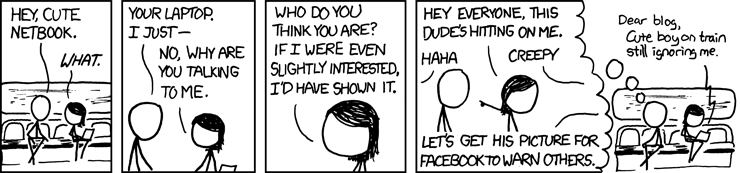
\includegraphics[width=\textwidth]{bilder/creepy.png}
}
\end{figure*}

Für viele Anruferinnen ist es sicherlich einfacher, sich erstmal ebenfalls an Studierende zu wenden, da sich diese in einer ähnlichen Lebenssituation befinden. Die Universität und das Studierendenwerk bieten ihren Studentinnen zwar eine professionelle Betreuung in der psychotherapeutischen Beratungsstelle, doch ist dazu zunächst eine Terminvereinbarung nötig, weshalb es Studierenden erstmal leichter fällt, bei der Nightline anzurufen. Hier kann man sofort, wenn der Schuh drückt, der Kummer überhand nimmt oder man während einer nächtlichen Lerneinheit eine kleine Sinnkrise erleidet anrufen und seinen Problemen Platz machen.

Generell werden sie aus ganz unterschiedlichen Gründen angerufen. Häufige Themen sind zum Beispiel Probleme mit Freunden oder Familie, Stress in der Uni oder Liebeskummer. Außerdem helfen sie auch gerne bei allgemeinen Fragen zur Uni oder zum Unileben weiter.

Einer der Grundpfeiler ihrer Arbeit am Telefon ist die Vertraulichkeit. Die Themen, die am Telefon angesprochen werden, bleiben innerhalb der Nightline und kursieren nicht darüber hinaus. Die Anrufende muss ihren Namen nicht nennen und auch die Nightlinerin stellt sich nicht persönlich vor. Dadurch wollen sie einen vorurteilsfreien und neutralen Raum schaffen. Die Anrufende bleibt vollkommen anonym – am Telefon der Nightline ist noch nicht einmal dessen Rufnummer zu sehen. Die bestehende Anonymität kann der Anrufenden helfen, ihr Problem offen auszusprechen ohne das Gefühl zu haben, sich auf irgendeine Art und Weise der Nightlinerin offenbaren zu müssen.

Im Grunde verstehen sie ihre Aufgabe im Zuhören. Ihnen ist es wichtig, vorurteilsfrei, anonym und vertraulich zu sein. Die Briten haben den Leitspruch: „We listen, not lecture!“ Daran halten sie sich auch. Ihre Aufgabe ist es nicht, Ratschläge zu erteilen, sondern zuzuhören. Die Nightline wird von zwei Diplompsychologen betreut, die eine Schulung für Nightliner durchführen und mehrmals im Semester Supervisionen abhalten. Sie sind ausgebildete Therapeuten und vermitteln ihre Kenntnisse über Gesprächsführung an sie weiter.

Prinzipiell versuchen sie immer zu helfen und zuzuhören, doch wenn sie merken, dass eine Anrufende mehr braucht, als sie bieten können, oder sie ihre eigenen Grenzen überschritten sehen, leiten sie, wenn dies gewünscht wird, an professionelle Dienste weiter. Dazu haben sie eine Sammlung von verschiedenen Beratungsstellen und~Nummern angelegt, um beispielsweise an Suchtberatungsstellen, Trauerbegleitungen und fremdsprachige Telefonseelsorgen weiter verweisen zu können.

Die Nightline besteht aus etwa 30 ehrenamtlichen Mitarbeiterinnen aus verschiedensten Fachbereichen. Das Geschlechterverhältnis ist nahezu ausgeglichen, so dass sich in der Nightline das breite Spektrum der Studierendenschaft widerspiegelt. Mitmachen kann jede, die bereit ist, sich ehrenamtlich zu engagieren und einen Teil ihrer Freizeit in den Dienst anderer zu stellen. Ein vorgegebenes Studienfach für Nightliner gibt es nicht.

Die Nightline ist während der Vorlesungszeit täglich zwischen 21 Uhr abends und 2 Uhr nachts unter der Nummer 0\,62\,21 / 18\,47\,08, via Skype unter \emph{nightline.heidelberg} oder über das Mailsystem unter \url{www.nightline-heidelberg.de} erreichbar.

\section{Studieren mit Handicap}
Die Beauftragten für behinderte und chronisch kranke Studierende beraten Studieninteressierte und Studentinnen der Uni Heidelberg in zentralen Fragen zum Studium mit gesundheitlicher Beeinträchtigung.
Das Angebot richtet sich an alle Studentinnen, die chronisch gesundheitlich eingeschränkt sind. Darunter fallen auch „unsichtbare“ Erkrankungen wie AD(H)S, Autismus, Legasthenie oder Depressionen. Generell gilt: Nicht die Diagnose, sondern der Hilfebedarf ist relevant.

Viele hilfreiche Informationen zum Angebot des Handicap-Teams, zu Ansprechpartnerinnen und Abläufen findet ihr bereits im Internet\footnote{\url{http://www.uni-heidelberg.de/studiummithandicap}}. Mit allen weiteren Fragen rund um das Thema Studium mit gesundheitlicher Beeinträchtigung, beispielsweise Fragen zur Gebäudezugänglichkeit,  zur Verfügbarkeit von speziellen Hilfsmitteln an der Universität oder zu diversen behinderungs- bzw. krankheitsbezogenen Anträgen, könnt ihr euch gerne per E-Mail an das Handicap-Team wenden. Ihr bekommt dann zeitnah Rückmeldung und könnt gegebenenfalls einen telefonischen oder persönlichen Beratungstermin vereinbaren.
Eure persönlichen Daten werden selbstverständlich vertraulich behandelt.

Studentinnen mit nachgewiesenen Beeinträchtigungen bei Prüfungen, zum Beispiel Legasthenie, Prüfungsangst oder Lese-Rechtschreib-Schwäche können unter Vorlage einer ärztlichen Bestätigung bei ihrem jeweiligen Prüfungsausschuss einen Nachteilsausgleich beantragen. Für Klausuren kann das zum Beispiel eine Schreibverlängerung sein.

\section{Physik-Buddy-Programm}
Das Buddy-Programm für Physikerinnen soll dich in deinem ersten Semester unterstützen und dir den Start ins Studium erleichtern. Du hast als Ersti die Möglichkeit, von zwei erfahrenen „Studien-Buddies“ begleitet zu werden, die dir und einer kleinen Gruppe von etwa 5 Studies im ersten Semester zur Seite stehen. 

Deine Buddies sind Ansprechpartnerinnen für dich. Bei Unsicherheiten kannst du dich jederzeit an sie wenden und mit sämtlichen Fragen löchern, sei es zum Studium, zur Uni, zum Studienverlauf oder zu allgemeinen Themen rund um das Leben in Heidelberg und vieles mehr. Unser Hauptziel ist es dabei, dich bestmöglich zu unterstützen. Daher haben wir verschiedene thematische Buddy-Gruppen, darunter solche für Erstakademikerinnen, Frauen für Frauen, LGBTQIA+ oder Neuankömmlinge in Deutschland. Natürlich kannst du dich aber auch für eine generelle Gruppe anmelden.

Deine Buddies lernst du dann bei einem ersten großen Treffen vor dem Vorkurs persönlich kennen.

Die Anmeldung für das Programm ist unkompliziert und erfolgt über das Übungsgruppensystem der Physik. Da kannst du gleich schonmal üben, dich wie für spätere Vorlesungen anzumelden. Wir informieren dich aber rechtzeitig vor Beginn mit allen relevanten Infos und dem Link zur Anmeldung über deine Uni-Mailadresse.


%%%%%%%%%%%%%%%%%%%%%%%%%%%%%%%%%%%%%%%%%%%%%%%%%%%%%%%%%%%%%%%%%%%%%%%%%%%%%
\chapter{An der Uni \dots}
% !TEX ROOT = ../ersti.tex
\section{EDV}

\subsection{Übersicht der digitalen Tools}
\label{digitale-tools-uebersicht}

Im Uni-Alltag benötigt ihr zahlreiche digitale Tools, die teilweise von der Universität selbst, teilweise von externen Anbietern gehostet werden. Dementsprechend sind sie manchmal frei zugänglich oder ihr benötigt einen Account; meist euren Uni-Account.

\begin{description}
    \item[\href{https://heico.uni-heidelberg.de/}{heiCO (Heidelberg Campus Online)}]
    Neues Campus-Management-System, das zukünftig für alle studentischen Angelegenheiten wie Bewerbung, Zulassung, Prüfungsanmeldung, Bescheinigungen etc. verwendet werden soll. Das System befindet sich aktuell im Aufbau und wird nach und nach eingeführt.

	\item[\href{https://lsf.uni-heidelberg.de/}{LSF (Lehre, Studium und Forschung)}]
    Informationssystem der Uni. Bietet aktuell alles, was mit Verwaltung zu tun hat: Vorlesungsverzeichnis, Informationen zu Personen, Gebäuden, Rückmeldung durchführen, Bescheinigungen ausdrucken. In Zukunft soll es (teilweise) durch heiCO ersetzt werden.

	\item[\href{https://moodle.uni-heidelberg.de}{Moodle}]
    E-Learning-Plattform der Uni, auf der in manchen Vorlesungen Lernmaterialien, Zettelabgaben, Punkteeinsicht, Klausuranmeldung und organisatorische Informationen angeboten werden.

	\item[\href{https://uebungen.physik.uni-heidelberg.de}{PhÜ (Physik-Übungruppen)}]
    Der Name ist Programm. Hier könnt ihr euch in der Physik in Übungsgruppen eintragen, zu Veranstaltungen anmelden sowie Punkte für Übungszettel und die Klausurnoten einsehen. Integriert Rocket-Chatrooms, die teilweise für die Kommunikation mit den Tutorinnen genutzt werden.

	\item[\href{https://muesli.mathi.uni-heidelberg.de}{MÜSLI}]
    In der Mathe und Info werden mit diesem System Übungsgruppen organisiert. Man kann sich in Übungsgruppen eintragen, zu Veranstaltungen und Klausuren anmelden und Punkte für Übungszettel und die Klausurnote einsehen.

	\item[\href{https://mampf.mathi.uni-heidelberg.de}{MaMpf (Mathematische Medienplattform)}]
    MaMpf bündelt und vernetzt verschiedene E-Learning-Angebote: Vorlesungsvideos und Skripte mit inhaltlicher Gliederung, Übungsblätter, eine umfangreiche Sammlung von Multiple-Choice-Fragen und Quizaufgaben inklusive angeleiteter Beweise und vieles mehr. Mehr Infos zu dieser Plattform auf \autopageref{mampf}.

	\item[\href{https://heiconf.uni-heidelberg.de}{heiCONF}]
    Uni-internes Videokonferenztool basierend auf BigBlueButton.

	\item[\href{https://meet.jit.si/}{Jitsi Meet}]
    Open-source Videokonferenztool.
\end{description}


\subsection{Universitätsrechenzentrum (URZ)}
\label{urz}
Computer sind die Triebfeder unseres Zeitalters und auch im Studium kommt ihr nicht um sie herum. Das beginnt zum Beispiel schon damit, dass die meisten Übungszettel nur online erscheinen und selbst ausgedruckt werden müssen. Später möchtet ihr eure Bachelor- oder Masterarbeit bzw.\ eure Examensarbeit sicher nicht handschriftlich anfertigen, sondern lieber in \LaTeX \footnote{„Latech“ gesprochen. LibreOffice -- oder noch schlimmer -- Word helfen nicht weiter, weil man Formeln nur sehr umständlich eingeben kann. Außerdem schafft es \LaTeX{} Blocktexte ohne größere Freiräume und mit weniger Bindestrichen zu setzen, wie man z.\,B.\ an diesem Ersti-Info sehen kann. Wenn ihr \LaTeX{} lernen möchtet, haltet in den nächsten Semestern nach einem entsprechenden Kurs Ausschau oder nutzt eins der vielen Onlinetutorials.} setzen. Das \gls{URZ} bietet eine ganze Menge von Services an, die hier kurz erläutert werden sollen.

\subsection{Campus Card}
\label{campuscard}

\begin{figure}[b]
    \centering
    \includegraphics[width=.75\linewidth]{bilder/planning.png}
\end{figure}

Wie an den meisten Unis ist der Studierendenausweis auch in Heidelberg voll modern und multifunktional. Neben der Ausweisfunktion wird er zum Ausleihen von Büchern in der Universitätsbibliothek und als \emph{Geldkarte} zum Bezahlen sowohl in der Mensa als auch an Kopierern und an einigen Waschstationen des Studierendenwerks benutzt. Um diese Funktion nutzen zu können, muss man Geld auf den Ausweis laden, dafür stehen in den Mensen Automaten zur Verfügung. Zusätzlich gilt der Ausweis im \gls{VRN} werktags ab 19 Uhr und an Wochenenden ohne Zeitbegrenzung auch als Fahrausweis (Details auf \autopageref{verkehrsmittel}).

Auf dem RFID-Chip der Karte ist nur die ID für die Bezahlfunktion des Studierendenwerks gespeichert und daher auch die einzige Information, die sich ohne Sichtverbindung auslesen lässt. Sofern euer Geldbeutel dünn genug ist und die Campus Card nicht durch Kleingeld, Bankkarten o.ä. abgeschirmt wird, lässt sich sogar durch Auflegen des Geldbeutels bezahlen -- allerdings sind die Lesegeräte nicht besonders stark und auch nicht besonders schnell, sodass ihr das am besten dann ausprobiert, wenn nicht so viel Betrieb ist. Alle anderen Informationen wie euer Name, die Matrikelnummer usw. sind lediglich aufgedruckt. Wichtig ist vor allem, dass euer Studierendenausweis auch validiert ist, sonst ist er nämlich nicht gültig. Diese Validierung müsst ihr jedes Semester nach eurer Rückmeldung durchführen, vergesst das nicht!

\subsection{Account}
Damit ihr überhaupt Zugang zum URZ bekommt, benötigt ihr Nutzername und Passwort. Euer Nutzername (Uni-ID) ist auf eurem multifunktionalen Studierendenausweis aufgedruckt. Um dann den Account nutzen zu können, muss die Uni-ID freigeschaltet\footnote{\url{https://online-services.urz.uni-heidelberg.de/id/uni_hd_account_activate.php}} werden. Hier könnt ihr auch euer Passwort und eure Uni-E-Mail-Adresse auswählen. Die Freischaltung kann man auch direkt beim Infoservice im URZ erledigen.

\vspace*{-2mm}
\subsection{E-Mail}
\vspace*{-1mm}
Mit der Freischaltung erhaltet ihr automatisch eine E-Mail-Adresse die auf \emph{@stud.uni-heidelberg.de} endet und momentan mit 1000 MB Speicherplatz nicht so schlecht ausgestattet ist. Größter Vorteil ist ihre Werbefreiheit und sehr gute Verfügbarkeit. \textbf{Achtung:} Solltet ihr die Adresse trotz allem nicht verwenden wollen, ändert \emph{unbedingt} eure Stammdaten im LSF\footnote{\url{https://lsf.uni-heidelberg.de}} und lasst euch die E-Mail-Adresse weiterleiten. Viele wichtige E-Mails wie die Rückmeldeerinnerung, Nachrichten von euren Tutorinnen oder Rundmails der Vorlesungen gehen dort ein.

%\begin{figure*}[b]
%    \centering
%    \begin{subfigure}{.2\textwidth}
%	    \includegraphics[height=3cm]{bilder/new_car_1.png}
%    \end{subfigure}
%    \begin{subfigure}{.2\textwidth}
%        \includegraphics[height=3cm]{bilder/new_car_2.png}
%    \end{subfigure}
%    \begin{subfigure}{.2\textwidth}
%        \includegraphics[height=3cm]{bilder/new_car_3.png}
%    \end{subfigure}
%    \begin{subfigure}{.2\textwidth}
%        \includegraphics[height=3cm]{bilder/new_car_4.png}
%    \end{subfigure}
%\end{figure*}

\vspace*{-2mm}
\subsection{Drucken}
\vspace*{-1mm}
Zum Drucken kann man seine Dokumente auf einen speziellen Druck-Server\footnote{\url{http://drucker.uni-hd.de}} laden und dann an (fast) jedem der über den Campus verstreut aufgestellten Kopiergeräte ausdrucken. Das zum Drucken benötigte Gut\-ha\-ben wird über die Campus Card abgerechnet, die man in den Mensen und in der \gls{UB} aufladen kann. Für größere Aufträge gibt es einen Druckerraum im Keller des \gls{URZ}, der von der Firma Ricoh betrieben wird. Darüber hinaus bietet das URZ einen Poster-Druckservice\footnote{\url{https://www.urz.uni-heidelberg.de/de/poster}} und einen 3D-Druckservice\footnote{\url{https://www.urz.uni-heidelberg.de/de/3d-druck}} an.

\vspace*{-2mm}
\subsection{CIP-Pools -- Internet ohne Notebook}
\vspace*{-1mm}
Rechnerräume gibt es im \gls{KIP} und im \gls{PI} im 1. Stock, in der Bibliothek im \gls{Mathematikon} und natürlich im \gls{URZ}, in letzterem sogar mehrere. Für Veranstaltungen stehen im Mathematikon auch noch weitere CIP-Pools bereit, diese sind aber üblicherweise nicht frei zugänglich.

\subsection{WLAN -- Internet mit Notebook}

\begin{figure}[h]
    \centering
    \vspace{-5mm}

    \ifthenelse{\boolean{druckversion}}{
        \includegraphics[width=\linewidth]{eduroam_sw.pdf}
    }{
        \includegraphics[width=\linewidth]{eduroam.pdf}
    }
    \vspace{-5mm}

\end{figure}

% \begin{figure*}[t]
%     \centering
%     \includegraphics[width=.8\textwidth]{bilder/computers_vs_humans.png}
% \end{figure*}



Am einfachsten und komfortabelsten ist der WLAN-Zugang über das e\-du\-roam-Netz. Die Uni Heidelberg beteiligt sich an der eduroam-Initiative und bietet jeder Rechenzentrums-Nutzerin einen entsprechenden Zugang. Damit könnt ihr nicht nur an vielen Stellen auf dem Campus kabellos ins Internet, sondern auch an mehreren hundert Hochschulen und Forschungseinrichtungen in über 60 Ländern – einfach so.

Wie ihr euer Notebook konfigurieren müsst, um eduroam zu nutzen, ist auf den Webseiten des URZ\footnote{\url{https://www.urz.uni-heidelberg.de/de/eduroam}} für die unterschiedlichsten Betriebssysteme sehr detailliert erklärt.

Neben eduroam bietet das URZ an einigen Stellen noch das Netzwerk „UNI-HEIDELBERG“, das man mit einem VPN-Zugang nutzen kann, sowie das unverschlüsselte „UNI-WEBACCESS“, bei dem man sich in einem Captive Portal authentifiziert.

Sollte euch der WLAN-Zugang nicht mehr ausreichen, gibt es an einigen Orten auch kabelgebundene Zugänge mit mehr Bandbreite. Wenn ihr jetzt schon feuchte Hände bekommt und euch die nigelnagelneue externe Platte mit Inhalten aus zweifelhaften Quellen vollladen möchtet, seid auf die Benutzerordnung\footnote{\url{https://www.urz.uni-heidelberg.de/de/dokumente/verwaltungs-und-benutzungsordnung-vbo/download}} verwiesen. Nach zu viel Traffic dreht euch das \gls{URZ} den Hahn ab und schaltet ihn erst wieder frei, wenn ihr bestätigt, dass ihr keine bösen Dinge damit anstellt.

\subsection{VPN}
Um auf manche Dienste zugreifen zu können, müsst ihr euch im internen Uni-Netz befinden. Weil das von zu Hause irgendwie schwer ist, braucht ihr einen VPN-Tunnel. Damit stellt euer Rechner über einen Internetzugang eine Verbindung zur Uni her und es ist so, als würdet ihr mit einem LAN-Kabel in der Uni sitzen. Eine ausführliche Anleitung findet ihr online\footnote{\url{https://www.urz.uni-heidelberg.de/de/vpn}}, die neben allgemeinen Informationen auch Anleitungen zur Installation des \emph{Cisco AnyConnect VPN Client}, enthält. Hier aber dennoch die Kurzfassung:

Unter Linux könnt ihr einfach \emph{openconnect} verwenden. Hier könnt ihr z.B. unter Ubuntu, Debian oder Mint das Paket \emph{network-manager-openconnect-gnome} nutzen und dort \emph{vpnsrv0.urz.uni-heidelberg.de} als Gateway und \emph{Deutsche\_Telekom\_Root\_CA\_2.pem} als CA Certificate einstellen, hier eine Anleitung\footnote{\url{https://youtu.be/_vOrUASbegs}}.

Unter Windows \ldots benutzt einfach kein Windows. Falls doch, nutzt den Cisco AnyConnect Client und folgt dieser Anleitung\footnote{\url{https://youtu.be/L6mlUyoEJ9I}}. Es gibt auch Alternativen, diese findet ihr auch auf den Seiten des Rechenzentrums.

\subsection{Lehre -- Studium -- Forschung (LSF)}
Das LSF\footnote{\url{https://lsf.uni-heidelberg.de/}} ist das Campus-Management-System der Uni. Hier findet ihr neben dem Vorlesungsverzeichnis und Informationen zu Gebäuden und Personen auch eure Bescheinigungen, beispielsweise für BAföG o.ä., euer Stammdatenblatt könnt ihr da auch ausdrucken. Das braucht ihr, um später nachweisen zu können, dass ihr auch wirklich studiert habt.

Für einige Funktionen braucht ihr eine TAN. Diese müsst ihr euch einmal als Liste ausdrucken. Das ist ein bisschen umständlich, sollte aber mit der Anleitung, die ihr bei eurer Einschreibung bekommen habt, kein Problem sein.

\subsection{Softwarelizenzen}

Über das URZ kann man als Studentin auch Lizenzen für verschiedene Programme und Betriebssysteme bekommen. Zum Beispiel Microsoft Office 365 Pro Plus. Die Uni ist Teil eines Abkommens von dem Land Baden-Württemberg mit Microsoft, wodurch alle Studentinnen sich das Office 365 Pro Plus Paket für \EUR{3.99} im Jahr holen können. Auch erwähnenswert ist Matlab, was für numerische Anwendungen ein praktisches Programm ist. Die gesamte aktuelle Liste findet ihr auf der URZ-Webseite\footnote{\url{https://www.urz.uni-heidelberg.de/de/service-katalog/software-und-anwendungen}}.

Außerdem gibt es diverse andere externe Dienstleisterinnen, die extra für Studentinnen besondere Konditionen anbieten. Zum Beispiel könnt ihr bei GitHub als Studentin unbegrenzt viele private Repositories kostenlos anlegen. Häufig ist für so etwas die \emph{@stud.uni-heidelberg.de}-Adresse notwendig.

\section{Bibliotheken}
\begin{table*}
    \centering

    % Diese Tabelle wurde mühsam angeordnet. Bitte nicht umbrechen, sondern scrollen!
    %~ \newcommand{\bibKIP}{}
    \begin{tabular}{lll@{ -- }l@{\quad}r@{ -- }l@{ Uhr}}
        \toprule
        \textbf{Name}                        & \textbf{Adresse}                                                                         & \multicolumn{4}{l}{\textbf{Öffnungszeiten}}                                                                                                       \\
        \midrule
        \multirow{5}{*}{\gls{UB} (Ausleihe)} & \multirow{2}{*}{\href{https://www.openstreetmap.org/?mlat=49.40966&mlon=8.70594&zoom=17&layers=M}{Plöck 107-109 (Altstadt)}} & Mo            & Fr & \ubAltAusMoFr       \\
                                             &                                                                                          & \multicolumn{2}{l}{Sa}                           & \ubAltAusSa                                                                                    \\[-0.7\defaultaddspace]
                                             & \multicolumn{1}{c}{}                                                                                                                                                                                                                         \\[-0.7\defaultaddspace]
                                             & \multirow{2}{*}{\href{https://www.openstreetmap.org/?mlat=49.41767&mlon=8.66836&zoom=17&layers=M}{INF 368, 3. Stock (Feld)}} & Mo            & Fr & \ubFeldAusMoFr      \\
                                             &                                                                                          & \multicolumn{2}{l}{Sa}                           & \ubFeldAusSa                                                                                   \\
        \cmidrule{1-6}
        \multirow{5}{*}{\gls{UB} (Lesesaal)} & \multirow{2}{*}{\href{https://www.openstreetmap.org/?mlat=49.40966&mlon=8.70594&zoom=17&layers=M}{Plöck 107-109 (Altstadt)}} & Mo            & Fr & \ubAltLesMoFr       \\
                                             &                                                                                          & Sa                                               & So           & \ubAltLesSa                                                                     \\[-0.7\defaultaddspace]
                                             & \multicolumn{1}{c}{}                                                                                                                                                                                                                         \\[-0.7\defaultaddspace]
                                             & \multirow{2}{*}{\href{https://www.openstreetmap.org/?mlat=49.41767&mlon=8.66836&zoom=17&layers=M}{INF 368 (Feld)}}           & Mo            & Fr & \ubFeldAusMoFr      \\
                                             &                                                                                          & Sa                                               & So           & \ubFeldAusSa                                                                    \\
        \cmidrule{1-6}
        \multirow{2}{*}{Mathematikon}        & \multirow{2}{*}{\href{https://www.openstreetmap.org/?mlat=49.41730&mlon=8.67580\#map=17/49.41730/8.67580}{INF 205}} & Mo           & Fr                                   & \mathekonMoFr                            \\
                                             &                                                                                          & \multicolumn{2}{l}{Sa}                           & \mathekonSa                                                                                    \\
        \cmidrule{1-6}
        \multirow{2}{*}{Physik}              & \multirow{2}{*}{\href{https://www.openstreetmap.org/?mlat=49.41479&mlon=8.69686&zoom=17&layers=M}{Philosophenweg 16}}        & Mo            & Fr & \physikMoFr         \\
                                             &                                                                                          & \multicolumn{2}{l}{}                             & \physikSa                                                                                      \\
        \cmidrule{1-6}
        \multirow{3}{*}{Stadtbücherei}       & \multirow{3}{*}{\href{https://www.openstreetmap.org/?mlat=49.40638&mlon=8.6866&zoom=17&layers=M}{Poststraße 15}}            & Di            & Fr & 10             & 20 \\
                                             &                                                                                          & \multicolumn{2}{l}{Sa}                           & 10           & 16                                                                              \\
                                             &                                                                                          & \multicolumn{4}{l}{Montags geschlossen!}                                                                                                          \\
        \cmidrule{1-6}
        \multirow{2}{*}{Studibücherei}       & \multirow{2}{*}{\href{https://www.openstreetmap.org/?mlat=49.41051&mlon=8.70518&zoom=17&layers=M}{Grabengasse 14}}           & Mo            & Do & 11             & 17 \\
                                             &                                                                                          & \multicolumn{2}{l}{Fr}                           & 11           & 14                                                                              \\
        \cmidrule{1-6}
        \multirow{2}{*}{Hinweis:}            & \multicolumn{4}{c}{\textbf{Während der vorlesungsfreien Zeit gelten veränderte Zeiten.}}                                                                                                                                                     \\
                                             & \multicolumn{4}{c}{\textbf{Bitte schaut dafür auf der jeweiligen Website nach.}}                                                                                                                                                             \\

        \bottomrule
    \end{tabular}

\end{table*}

Fachliteratur ist meistens unglaublich teuer. Um den totalen Ruin der Studierenden zu vermeiden, hat jede Universität Bibliotheken. In Heidelberg ist die \gls{UB} dreigeteilt, und zwar entsprechend der Dreiteilung der Universität. Die für euch wahrscheinlich interessanteste Literatur über Mathe, Informatik und Physik befindet sich in der Zweigstelle \gls{INF}~368, 3.~Stock.


Neben Physik-, Informatik- und Mathebüchern können hier auch medizinische Literatur und Bücher für alle anderen Fakultäten, die im Neuenheimer Feld untergebracht sind, ausgeliehen werden. Im Hauptsitz der \gls{UB} an der Peterskirche, Plöck~107-109, und der Campus-Bibliothek in Bergheim hingegen findet sich geisteswissenschaftliche Literatur sowie zahlreiche Jura- und VWL- Bücher. Bedingt durch diese Dreiteilung wurde in Heidelberg sehr früh ein Computersystem (\gls{HEIDI}\footnote{\url{https://katalog.ub.uni-heidelberg.de}}) in der UB eingeführt. Mit Hilfe von HEIDI und eurer Uni-ID, die auf eurem Studiausweis steht, kann dort die gängige Fachliteratur ausgeliehen werden. Übers Internet lässt sich auch direkt nach Büchern suchen, außerdem können ausgeliehene Bücher online verlängert werden -- das kann einem durchaus den einen oder anderen Euro sparen, die Mahngebühren bei überzogenen Fristen sind nämlich empfindlich teuer. Viele Bücher lassen sich auch als PDF downloaden oder wenigstens als E-Book online abrufen. Zu Semesterbeginn finden in der UB Einführungskurse in HEIDI statt, die jedoch nur bedingt sinnvoll sind, weil das System sehr übersichtlich und intuitiv aufgebaut ist und sich größtenteils selbsterklärend bedienen lässt.

So ist es bspw. möglich, über die Suche festzustellen, ob ein Buch als E-Book aufrufbar ist. Der jeweilige Sucheintrag enthält dann links-unten einen „Online-Ressource“-Hinweis. Auf der jeweiligen Seite des Buches findet sich dann links-oben ein Link „online aufrufen“, der zu der E-Book-Version führt, nachdem du „Universität Heidelberg“ angewählt und dich mit deiner Uni-ID angemeldet hast.

Mittels HEIDI lassen sich auch Gruppenarbeitsräume in den Bibliotheken kostenfrei reservieren, was insbesondere praktisch für das Zettellösen in Gruppenarbeit am Wochenende ist.

Wer weiterführende spezielle Fachliteratur sucht, muss sich an die Bereichsbibliotheken der einzelnen Fakultäten richten, deren Bestände ebenfalls in \gls{HEIDI} erfasst sind. Für Mathe- und Informatik-Literatur befindet sich die Bereichsbibliothek im Gebäude \gls{INF}~205 (im Erdgeschoss auf der Ostseite). Weitere Informationen und Öffnungszeiten finden sich auf der Webseite der Bereichsbibliothek.\footnote{\url{https://www.mathinf.uni-heidelberg.de/de/facultylibrary}} Spezielle Physikbücher findet man an den Standorten der Bereichsbibliothek Physik und Astronomie (BPA), welche ihren zentralen Sitz am Philosophenweg~16 hat.\footnote{\url{https://www.ub.uni-heidelberg.de/dezentral/bpa/standorte.html}} Auch wenn die Lage etwas abschreckend wirken mag, lohnt sich ein Besuch, alleine wegen des Gebäudes. Die Bibliothekarinnen freuen sich sehr über studentischen Besuch. Die Bereichsbibliothek der Physik führt auch weitere Standorte in einzelnen Instituten, hier kommt man jedoch erst nach Vereinbarung rein.
Bei den Bereichsbibliotheken handelt es sich um Präsenzbibliotheken. Das bedeutet, dass man Bücher und Zeitschriften vor Ort kopieren, aber nicht ausleihen, darf. Für die Ausleihe spezieller Werke können jedoch auch Ausnahmen gemacht werden, z.B. im Falle eines für eine Abschlussarbeit notwendiges Buches, welches nur in der Bereichsbibliothek geführt wird.
Wenn ein Buch in der UB komplett ausgeliehen ist, dann lohnt es sich manchmal auch, zur Stadtbücherei in der Poststraße zu gehen. Zum Anmelden braucht man nur einen Personalausweis. Die Ausleihe ist allerdings nicht kostenlos (\EUR{10}/Jahr). Weitere Information kannst du auch direkt bei der Stadtbücherei einholen.\footnote{\url{https://www.heidelberg-stadtbuecherei.de}}

Solltest du Werke in physischer oder digitaler Form vermissen, so kannst du über das Anschaffungsvorschlagsformular der Universitätsbibliothek\footnote{\url{https://www.ub.uni-heidelberg.de/allg/benutzung/bereiche/vorschlag.html}} Vorschläge einbringen. Für physiknahe Werke kannst du dich auch an uns als Fachschaft wenden, da in der Physik ein Bibliotheksausschuss existiert, in welchem auch eine studentische Vertreterin, genau für solche Zwecke, sitzt.

% \begin{figure*}[t]
% \centering
% \includegraphics[width=\textwidth]{bilder/library.png}
% \end{figure*}


% -> Could not find website of Studibücherei anymore: https://www.stw.uni-heidelberg.de/de/studibuecherei. Maybe this offer does not exist anymore?
%
% Das Studierendenwerk bietet zusätzlich noch die Studierendenbibliothek\footnote{\url{https://www.studentenwerk.uni-heidelberg.de/de/studibuecherei}}, welche neben geistenswissenschaftlicher Fachliteratur auch insbesondere Welt-, Kriminial- und Unterhaltungsliteratur in ihrem Bestand hat. Die Studierendenbibliothek, wie auch die Stadtbücherei laden dazu ein, neben der ganzen Studiererei auch einfach mal abzuschalten und zu schmökern.

\section{Physik-Helpdesk}
\label{sec:physik-helpdesk}

Seit einigen Jahren gibt es in der Physik einen Helpdesk (bis vor einem Jahr hieß dieser „Studentischer Arbeitsraum“). Dort findest du eine Tutorin aus einem höheren Semester, die dir bei Fragen zu Übungszetteln, zu Vorlesungsinhalten und zum Physikstudium ganz allgemein weiterhelfen kann. Die Tutorin ist kein Quell für Musterlösungen, sondern kann dir durch ihre eigene Studienerfahrung bei Problemen und Unklarheiten aller Art weiterhelfen und Tipps geben. Insgesamt lässt sich sagen, dass der Physik-Helpdesk in dieser Hinsicht ein niederschwelliges Zusatzangebot zu den Übungsgruppen ist. Außerdem findest du beim Helpdesk auch eine Auswahl an Lehrbüchern als kleine Präsenzbibliothek, und kannst dir sehr preiswert einen Kaffee oder einen Tee machen.

Zu finden ist der Physik-Helpdesk im \gls{KIP} im zweiten Stock vor den Seminarräumen. Von der zweiten bis zur vorletzten Vorlesungswoche sitzt dort montags bis freitags von 13 bis 19~Uhr eine Tutorin, die du auch durch ein großes Plakat an der Wand erkennen kannst. Die aktuellen Infos zum Helpdesk sollten auch immer hier\footnote{\url{https://uebungen.physik.uni-heidelberg.de/arbeitsraum}} zu finden sein.

Falls du also mal an einem Übungszettel verzweifeln solltest, komm vorbei und lass dir helfen.

% !TEX ROOT = ../ersti.tex

\vspace{-2mm}
\section{Die kleine BAföG-Liste}

\paragraph{Was ist BAföG überhaupt?}
BAföG ist eine Abkürzung für \glqq{}Bundesausbildungsförderungsgesetz\grqq{}, das Gesetz, das in Deutschland die staatliche Unterstützung für die Ausbildung von Schülerinnen und Studentinnen regelt. Ziel des BAföG ist es, jungen Menschen unabhängig von ihrem sozialen und finanziellen Hintergrund eine (schulische) Ausbildung oder ein Studium zu ermöglichen. Dafür kannst du einen \glqq{}Antrag auf Ausbildungsförderung\grqq{} stellen, um, wenn du bestimmte Voraussetzungen erfüllst, finanzielle Unterstützung zu erhalten. 

Wer von BAföG spricht, meint meistens nicht das Gesetz, sondern genau diese finanzielle Förderung.

\vspace{-2mm}
\paragraph{Soll ich BAföG beantragen?}
JA! Ob du anspruchsberechtigt bist, ist für dich meistens nicht so einfach zu erkennen, deswegen stelle auf jeden Fall einen Antrag. Wenn dieser abgelehnt wird, hast du höchstens ein wenig Zeit verloren, wenn nicht, lohnt es sich für dich ziemlich sicher:

Für dich als Studi sind 50\% der Förderung Zuschuss, die andere Hälfte zinsloses Darlehen. Zurückzuzahlen ist dieses Darlehen frühestens fünf Jahre nach Studienabschluss, aber nur ab einer bestimmten Einkommenshöhe. Unter bestimmten Voraussetzungen (z.\,B. Versorgung eines Kindes) ist auch sonst ein Rückzahlungsaufschub möglich. Außerdem kann (z.\,B. bei besonders guten Studienleistungen oder frühzeitiger Rückzahlung) ein Nachlass auf die Darlehensschuld gewährt werden.

\vspace{-2mm}
\paragraph{Wie viel gibt es und wie lange und ab wann?}
Für Studierende ohne Kinder gibt es bis zu \bafoeghoechstsatz. Wie hoch der monatliche Förderungsbetrag ist, hängt ab von Mietverhältnis, Einkommen der Eltern, eigenem Vermögen, Krankenversicherung, Geschwistern, etc. Die Förderungsdauer richtet sich nach der Regelstudienzeit (Bachelor und konsekutiver Master = 6 + 4 Semester, aber es gibt fachspezifische Ausnahmen). Die Anspruchszeit zählt ab Immatrikulation und ist nicht aufsparbar! Die Auszahlung geschieht in der Regel erst, wenn der Bescheid bei euch eingegangen ist, bei dringender Bedürftigkeit ist ggf. ein Vorschuss in voller BAföG-Höhe, der hinterher verrechnet wird, möglich.

\vspace{-2mm}
\paragraph{Wo und bis wann muss ich den Antrag stellen?}
Das geht beim BAföG-Amt des Studierendenwerks im Marstallhof 3 oder in der Kurzberatung im Neuenheimer Feld\footnote{Öffnungszeiten siehe \url{https://www.stw.uni-heidelberg.de/de/bafoeg_kontakt}}. Das macht man am besten, sobald man die Immatrikulationsbescheinigung hat, denn BAföG gibt es erst vom Antragsmonat an, wobei der frühestmögliche Termin der Semesteranfang ist.

\vspace{-2mm}
\paragraph{Was muss ich beim Antrag beachten?}
Wichtig ist, den Antrag so früh wie möglich zu stellen, weil es teilweise zu langen Bearbeitungszeiten kommen kann. Der Antrag sollte idealerweise gleich vollständig sein, damit keine Rückfragen an dich nötig sind und der Antrag schneller bearbeitet werden kann. Ansonsten gilt: lieber schnell beantragen und Papiere nachreichen. Die Angaben sollten selbstverständlich wahrheitsgemäß sein, denn das Amt kann die Finanzdaten prüfen.

\vspace{-2mm}
\paragraph{BAföG und nun?}
Man muss nach dem vierten Fachsemester seine Studienleistungen bescheinigen lassen. Wichtig ist außerdem,  familiäre und persönliche wirtschaftliche Veränderungen immer sofort zu melden (Schwester/Bruder in Ausbildung/Arbeit, Arbeitslosigkeit, etc.). Es gibt auch Auslands-BAföG und viele sonstige Ausnahmen, zu denen man sich am besten beraten lässt, denn es kann sich lohnen! Eigener Zuverdienst ist jedoch nur begrenzt möglich.

\noindent Abschließend: Bei BAföG durchzublicken ist gar nicht so einfach, und auch uns ist das noch nicht hundertprozentig gelungen. Deswegen können sich auch in diesem Text Fehler eingeschlichen haben. Wir wollen an dieser Stelle aber auch gar keine allumfassende Anleitung für BAföG verfassen, sondern vor allem erreichen, dass du dich selbst informierst. Am sinnvollsten ist es, wenn du dich selbst mit dem Thema beschäftigst und dich beraten lässt.

Nutze hierzu die Sprechstunde vom Sozialreferat des \gls{StuRa}\footnote{\url{https://www.stura.uni-heidelberg.de/vs-strukturen/referate/soziales/}}. Die helfen beim Antrag, erklären Ausnahmen und geben Tipps um spätere Probleme zu vermeiden, bei denen sie natürlich auch helfen.

% !TEX ROOT = ../ersti.tex
\section{Studium im Ausland}
Man hört immer wieder von den tollen Erfahrungen und Möglichkeiten, die ein Studium im Ausland bietet. Die Leute schwärmen davon, wie schön es an der Uni so-und-so war. Aber wie kommt man überhaupt dahin?

Auf der Homepage der jeweiligen Fakultät findet ihr eine Liste von Unis, mit denen Austauschprogramme laufen, zum Beispiel über ERASMUS oder bilaterale Abkommen, die also üblicherwiese anerkannt werden, einige generelle Infos und ein paar Erfahrungsberichte, die ihr bei Interesse anschauen solltet. Die Gleichwertigkeit von Studienleistungen muss allerdings nicht von euch überprüft werden, die Beweispflicht liegt bei der Fakultät. Lasst euch also nicht beirren und hört im Zweifel die Veranstaltung im Ausland einfach, die sollen erst mal zeigen, dass das nicht das Gleiche war.

Allerdings sollte ein Auslandssemester im Moment nicht euer erstes Problem sein -- während der ersten beiden Semester ist es ganz einfach fachlich nicht möglich. Bis zur Einführung der Bachelor- und Masterstudiengänge konnte man -- jedenfalls in der Mathe -- an diesen Programmen nur nach abgeschlossenem Grundstudium teilnehmen, inzwischen wird der Zeitraum letztes Bachelor Jahr\,/\,erstes Master Jahr empfohlen. Das bedeutet, dass ihr nach dem zweiten Semester damit beginnen solltet, euch umzuschauen, insbesondere in Bezug auf Bewerbungsvoraussetzungen und -fristen.

Auslands-BAföG müsst ihr übrigens separat beantragen, das zu\-stän\-dige Amt dafür hängt vom jeweiligen Ausland ab\footnote{\url{https://www.auslandsbafoeg.de/}}. In Heidelberg kann man sich auch direkt an das Dezernat Internationale Beziehungen, früher Akademisches Auslandsamt, (AAA)\footnote{\url{https://www.uni-heidelberg.de/einrichtungen/verwaltung/internationales/}} wenden, das ihr in der Seminarstraße 2 findet. Ihr müsst dann ins Auslandsstudium Info-Zimmer 139\footnote{Öffnungszeiten: \auslandsinfooeff}.

Sehr wichtig ist noch zu wissen, dass man Urlaubssemester beantragen kann, damit die Fachsemesterzahl -- vor allem wichtig für alle, die Inlands-BAföG erhalten -- nicht weiter läuft. Dafür läuft die Hochschulsemesterzahl weiter. Man kann sich dann die im Ausland erworbenen \gls{LP} -- nach Absprache mit dem Prüfungssekretariat -- anrechnen lassen.

Für das Urlaubssemester ist die Studierendenadministration in der Seminarstraße 2 zuständig. Mehr Infos und das Formular zum Urlaubssemester findet ihr online\footnote{\url{https://www.uni-heidelberg.de/studium/imstudium/formalia/beurlaubung.html}}.


% !TEX ROOT = ../ersti.tex
\section{heiSKILLS}

heiSKILLS unterstützt euch dabei, eure Kompetenzen im Studium und darüber hinaus zukunftsfähig zu gestalten und zu erweitern. Das heiSKILLS Kompetenz- und Sprachenzentrum vereint hierfür die Beratungs- und Veranstaltungsangebote des Zentralen Sprachlabors, des Career Service sowie Study Skills für das Lernen, um euch so für euer Studium zu stärken und euch auf eure berufliche Zukunft vorzubereiten.

\begin{itemize}[leftmargin=3mm]
  \item Möchtet ihr wissenschaftliches Schreiben üben oder eure Kompetenzen im kritischen Denken erweitern?
  \item Leitet ihr ein Tutorium und wollt euch fit machen, wie ihr Kommilitoninnen beim Lernen unterstützen könnt?
  \item Möchtet ihr Fremdsprachenkenntnisse ausbauen oder neu erwerben und benötigt international anerkannte Sprachnachweise für euer Studium oder einen Auslandsaufenthalt?
  \item Benötigt ihr eine starke Stimme für euren zukünftigen Beruf, etwa als Lehrerin, und möchtet zudem eure rhetorischen Fähigkeiten fördern?
  \item Wollt ihr euch im Rahmen von Karriereveranstaltungen vernetzen, informieren und mit unseren Expertinnen über mögliche Berufsperspektiven und -optionen sprechen oder euch in einer individuellen Karriereberatung hinsichtlich beruflicher Perspektiven coachen lassen?
  \item Seid ihr interessiert daran euch während des Studiums berufsrelevante Zusatzqualifikationen wie z.\,B.\, betriebswirtschaftliche Grundlagen, Projektmanagement oder Medienproduktion zur Schärfung Eures Kompetenzprofils anzueignen?

\end{itemize}

Möglichkeiten hierzu, aber auch zu vielem mehr findet ihr bei heiSKILLS.
Eine Liste der Angebote gibt es im LSF und auf den Abteilungswebseiten\footnote{\url{https://www.uni-heidelberg.de/careerservice/veranstaltungen}, \url{https://www.uni-heidelberg.de/slk/nutzbar/}}.
Falls ihr Fragen, Vorschläge oder Ideen für weitere Angebote habt gebt einfach Bescheid unter \email{heiSKILLS@uni-heidelberg.de}. Das heiSKILL-Team freut sich, von euch zu hören und euch in deren Kurse und Veranstaltungen zu sehen!

% !TEX ROOT = ../ersti.tex
% \vfill\eject

\section{Werk- und Experimentierraum}
\label{werk-und-experimentierraum}

Um deinen Erfindergeist und dein handwerkliches Geschick zu fördern, wurde der studentische Werk- und Experimentierraum gegründet. Dieser Raum bietet dir die Möglichkeit, unter Aufsicht und mit der Unterstützung erfahrener Tutorinnen eigene Projekte selbstständig durchzuführen und dabei die universitären Strukturen frühzeitig kennenzulernen und zu nutzen. Zudem werden regelmäßig Workshops zu spannenden Projekten wie dem Bau von Fahrzeugen organisiert.

Der Raum ist mit einer Vielzahl an Werkzeugen und Geräten ausgestattet: von Elektronik- und mechanischen Werkzeugen über 3D-Drucker, Arduinos, Raspberry Pi und Asuros inklusive kompatibler Sensoren und Module bis hin zu Holz- und Metallverarbeitungswerkzeugen und einer Nähmaschine.

Um den Werkraum nutzen zu können, ist eine Sicherheitseinweisung erforderlich, die jedes Semester angeboten wird. Informationen zu Öffnungszeiten, Anmeldung, Ansprechpartnerinnen und dem Standort findest du auf der Webseite\footnote{\url{https://www.kip.uni-heidelberg.de/mitarbeit/werkraum%7D%7D.

Der Raum steht dir offen, auch wenn du keine Physikstudentin bist. Wenn du Lust hast, an eigenen Projekten zu arbeiten, etwas Cooles zu bauen oder einfach etwas Neues zu lernen, ist der Werkraum genau der richtige Ort für dich!

% !TEX ROOT = ../ersti.tex
% \vfill\eject
\section{Weitere Angebote}

\subsection{Mathematik-Mentorinnenprogramm \\Upstream}
Das Interdisziplinäre Zentrum für Wissenschaftliches Rechnen (IWR) an der Uni Heidelberg bietet seit 2013 mit Upstream\footnote{\url{https://www.mathcomp.uni-heidelberg.de/programs/upstream}} ein Mentorinnenprogramm für Mathematik-interessierte Frauen. Upstream ist ein Netzwerk für junge Mathematikerinnen in allen Stufen der Ausbildung -- von Schülerinnen ab der 10. Klasse, Studentinnen, Doktorandinnen, Nachwuchswissenschaftlerinnen bis hin zu Professorinnen. In regelmäßigen Abständen organisieren wir Meet\,\&\,Greet-Treffen, Public Lectures, Diskussionsrunden und Workshops zu Themen, in denen Schlüsselqualifikationen und studiengangsspezifische Inhalte vermittelt werden. Dabei nehmen erfahrene Mathematikerinnen die Mentorinnenrolle ein. Sie stehen den Teilnehmerinnen zur Seite, beraten und beantworten Fragen rund um das Studium und das Berufsleben.

Wenn du Mitglied werden willst, schicke einfach etwa eine halbe Seite Motivationsschreiben per E-Mail an: \email{upstream@iwr.uni-heidelberg.de}. Die Aufnahme in das Programm ist nicht an Noten oder Wettbewerbserfolge geknüpft; wir suchen vor allem begeisterte Mathematikerinnen auf allen Ebenen.

\subsection{Kooperationsabkommen mit der \\Universität Mannheim}
Zwischen der Universität Heidelberg und der Universität Mannheim gibt es ein Kooperationsabkommen, was Studierenden in Mathematik, Informatik und Physik ermöglicht, kostenlos als Gaststudentin Vorlesungen an Fakultät für Wirtschaftsmathematik und Wirtschaftsinformatik zu hören und sich hier in Heidelberg anrechnen lassen.
Somit kann man das vielfältige Vorlesungsangebot nutzen und insbesondere Module wie Kryptographie, angewandte Algebra und Spieltheorie belegen, die so nicht in Heidelberg angeboten werden.

%%%%%%%%%%%%%%%%%%%%%%%%%%%%%%%%%%%%%%%%%%%%%%%%%%%%%%%%%%%%%%%%%%%%%%%%%%%%%
\chapter{\dots und in der Stadt}
% !TEX ROOT = ../ersti.tex

\section{Wohnen in Heidelberg}

Wie in jeder Unistadt, so ist es auch in Heidelberg schwer, zu Anfang des Semesters ein Zimmer zu finden, das bezahlbar ist und möglichst zentral liegt. Im Durchschnitt muss man in Heidelberg mit Lebenshaltungskosten von ca. \lebenshaltungskosten (inklusive Miete) pro Monat rechnen.

\begin{figure*}[t]
    \centering
    \begin{subfigure}{.3\textwidth}
        \includegraphics[height=4.5cm]{bilder/travelling_salesman_problem_1.png}
    \end{subfigure}
    \begin{subfigure}{.3\textwidth}
        \includegraphics[height=4.5cm]{bilder/travelling_salesman_problem_2.png}
    \end{subfigure}
    \begin{subfigure}{.3\textwidth}
        \includegraphics[height=4.5cm]{bilder/travelling_salesman_problem_3.png}
    \end{subfigure}
\end{figure*}

Am günstigsten wohnt man immer noch im Studierendenwohnheim, dort muss man mit Mieten von ca.~\studentenwohnheim pro Monat rechnen. Eine frühzeitige Bewerbung ist hier dringend notwendig. Auch WG-Zimmer sind teilweise recht günstig zu bekommen, in der Regel jedoch teurer als ein Zimmer im Wohnheim und oft nicht lange im Voraus zu reservieren.

Die Idee, eine eigene WG zu gründen, liegt meist sehr nahe, jedoch wird man schnell merken, dass das gar nicht so einfach ist. Oft werden Ehepaare ohne Kinder bevorzugt oder ein Zimmer entpuppt sich als Durchgangszimmer. Egal für was ihr euch entscheidet: Plant viel Zeit ein und lasst nicht locker!

Nun aber zur konkreten Zimmersuche: Es gibt mehrere Möglichkeiten, ein Zimmer in Heidelberg zu finden. Das Studierendenwerk bietet mehrere Anlaufstellen: In der Altstadt das Info-Café International in der Triplex-Mensa direkt am Uniplatz, im Neuenheimer Feld im Infocenter der Zentralmensa. In den Mensen, aber auch in den einzelnen Instituten empfiehlt es sich, die schwarzen Bretter abzuklappern und nach privaten Aushängen Ausschau zu halten oder selbst Anfragen anzuhängen. Weitere gute Quellen für Zimmerangebote sind natürlich die regionalen Zeitungen. Das wären u.a. \emph{Sperrmüll}, erscheint immer dienstags und freitags und die Rhein-Neckar-Zeitung, mittwochs und samstags mit großem Immobilienteil. %Aufpassen müsst ihr bei Makler-Vermittlungen, hier müsst ihr zusätzlich zwischen %ein und zwei Monatsmieten Provision zahlen. Eine eigene Anzeige kann natürlich nie schaden. Zu guter Letzt gibt es noch das Internet, das eine Fülle an Portalen\footnote{z.B. \url{wg-gesucht.de}} zur Wohnungssuche bietet.


\subsubsection{Wohnheime}

%\begin{figure*}[t]
%    \centering
%    \begin{subfigure}{.2\textwidth}
%    \includegraphics[height=4.5cm]{bilder/household_tips_1.png}
%    \end{subfigure}
%    \begin{subfigure}{.25\textwidth}
%    \includegraphics[height=4.5cm]{bilder/household_tips_2.png}
%    \end{subfigure}
%    \begin{subfigure}{.2\textwidth}
%    \includegraphics[height=4.5cm]{bilder/household_tips_3.png}
%    \end{subfigure}
%    \begin{subfigure}{.28\textwidth}
%    \includegraphics[height=4.5cm]{bilder/household_tips_4.png}
%    \end{subfigure}
%\end{figure*}

In und um Heidelberg gibt es ca. 50 Wohnheime des Studierendenwerks, im Wintersemester werden ca. ein Fünftel aller dieser Zimmer neu vermietet. Die Auswahl erfolgt nach sozialen Kriterien wie zum Beispiel Heimatferne, Verdienst der Eltern, Wohnverhältnisse usw. Die Wohnzeit ist auf sechs Semester begrenzt, aber es gibt viele Möglichkeiten, diese zu verlängern, zum Beispiel durch Sonderaufgaben im Wohnheim, Härtefälle, Engagement in der Fachschaft, etc. Die maximale Wohnzeit kann auf insgesamt zehn Semester ansteigen, was durchaus vorkommt. Je nach Wohnheim gibt es Einzelzimmer mit Stockwerksküche und -bad, die ihr dann mit jeweils 15-20 Leuten teilt -- was mittlerweile aber eher selten ist -- Einzelzimmer in 2er, 3er oder 4er WGs oder sogar Einzelappartments. Die Zimmer sind in der Regel nicht sehr groß (11--16 \squaren\metre), aber ausreichend. Nachteile von Wohnheimen können die teilweise sehr unterschiedlichen Vorstellungen von Hygiene sein, ein hoher Lärmpegel und immer wieder neue Überraschungen. Allerdings bietet ein Wohnheim vor allem für Leute, die neu in der Stadt sind, den großen Vorteil, sehr schnell viele Leute kennen zu lernen, außerdem muss man sich um Reparaturen nicht selbst kümmern. Es gibt keine konkreten Bewerbungsfristen. Die Bewerbung sollte allerdings bis 1. Juli für das Wintersemester und bis 1. Januar für das Sommersemester eingegangen sein, weil dann mit der Zimmereinteilung und dem Versand der Mietverträge begonnen wird. Später eingehende Bewerbungen haben weitaus geringere Chancen und Auswahlmöglichkeiten. Antragsformulare gibt es in den Infocentern des Studierendenwerks oder im Internet\footnote{\url{https://www.studierendenwerk.uni-heidelberg.de}}. Dort gibt es auch eine vollständige Liste aller Wohnheime des Studierendenwerks. Auch private, kirchliche oder sonstige Träger bieten Zimmer in Wohnheimen an, für diese müsst ihr euch direkt beim Wohnheim bewerben, nicht beim Studierendenwerk. Eine Liste findet ihr aber beim Studierendenwerk\footnote{\url{https://www.stw.uni-heidelberg.de/sites/default/files/download/pdf/wo-in-hd-andere-traeger-de.pdf}}.

% !TEX ROOT = ../ersti.tex
\newcounter{zahl}
\newcommand{\place}[4]{\item[(\stepcounter{zahl}\thezahl) #1](#2)\\ #3\\\emph{Preis:} #4}

% Indikator für Frauenanteil? Nein!

\section{Bars, Kneipen \& Diskotheken}
$\star$ teuer\quad $\star\ \star$ noch teurer \quad $\star\ \star\ \star$ extrem teuer

% trim=l b r t
%\hspace*{-6mm}
\begin{figure*}
    \altstadtkarte
\end{figure*}

\subsection{In der Altstadt:}
\begin{description}

    %   \place{Alfredo}{Untere Straße}{Wirklich sehr leckere Pizza, der Chef sorgt für den echt italienischen Flair.}{$\star$}

    \place{Destille}{Untere Straße 16}{Besondere Shots, die jede in Heidelberg mal probiert haben sollte (\emph{Warmer Erpel}~\&~\emph{Gehängter}). Selbst an Tagen, an denen die Untere Straße leer ist, tanzen hier Leute auf den Tischen.}{$\star\ \star$}

    \place{Sonderbar\,/\,Betreutes Trinken}{Untere Straße 13}{Jede nur erdenkliche Form von Absinth, auch viel guten Rum und Whisky. Immer ordentlich was auf die Ohren (Hard\,\&\,Heavy). Keine Angst vor dem Wirt, einfach nicht auf den Mund gefallen sein. Oft sehr voll und vollgeräuchert.}{$\star\ \star$}

    \place{Eckstein}{am Fischmarkt 3}{Abgefahrene Kneipe. Je nach Wochentag ändert sich das Programm. Es gibt jedoch immer einen Kicker und reichlich Platz. Drei Mal wöchentlich Zaubershows.}{$\star\ \star$}

    \place{Mohr}{Untere Straße 3}{Spät abends meist so voll, dass man gar nicht mehr rein kommt. Drinnen wird dafür allerdings auf den Tischen getanzt. Donnerstags gibts zur Ladies’ Night kostenlosen Sekt für die Damen.}{$\star\ \star$}

    \place{Palmbräugasse}{Hauptstraße 185}{Hier gibts das selbstgebraute Palmbräu. Palmen gehören zwar nicht typisch zu Heidelberg, aber die Schnitzel in der Palm\-bräu\-gasse.}{$\star\ \star\ \star$}

    \place{Reichsapfel \& Lager}{Untere Straße 35}{Sehr geräumig. Moderner Vorderbereich und urigere Atmosphäre im hinteren Teil, welcher über den Innenhof zugänglich ist. Dort findet man oft Platz, wenn sonst alles voll ist.}{$\star\ \star$}

    \place{Mels}{Heiliggeiststraße 1}{Gewölbekeller, in dem seit Jahren die selbe Musik läuft, aber zumindest weiß man dann, was einen erwartet. Haben unter der Woche immer sehr gute Spezialangebote z.B. dienstags 123-Party (Bier \EUR{1}, Weizen \EUR{2}, Cocktails \EUR{3}).}{$\star\ \star$}

    \place{Cave 54}{Krämergasse 1}{Deutschlands ältester Jazzkeller. Kostet am Wochen\-ende Eintritt, hat dafür allerdings noch nach 3 Uhr geöffnet.}{$\star\ \star$}

    \place{Coyote Café}{Hauptstraße 130}{Einer der Orte, um eine Kneipentour durch die Altstadt starten zu lassen. Weizenbier, Cocktails und Shots sind brauchbar und brauchen nicht ewig. Am späteren Abend gibt es häufig eine Happy Hour, bei der Cocktails nur die Hälfte kosten.}{$\star\ \star$}

    %\place{Hard Rock Cafe}{Hauptstraße 142}{Montags Bier für \EUR{1}, ab 18 Uhr Cocktails für \EUR{4}. Musik wie man es erwartet, durchgehend Rock.}{$\star$}
    \place{Ben's Burgerbar}{Hauptstraße 142}{Hieß früher mal Hard Rock Cafe. Ab 18 Uhr Cocktails für \EUR{4}. Musik wie man es erwartet, durchgehend Rock.}{$\star$}

    %    \place{Havanna}{Neckarstaden 24}{Cocktailbar mit Möglichkeit zum Salsa tanzen.}{$\star\ \star\ \star$}

    \place{Hemmingways}{Fahrtgasse 1}{Hier lässt es sich das gesamte Jahr draußen sitzen, dank warmen Decken und Heizstrahlern. Außerdem kann man wunderbar den Neckar beobachten.}{$\star\ \star$}

    \place{Karl}{Lauerstraße 7-9}{Kneipe mit Kicker und Dartscheiben. Manchmal mit Live-Musik.}{$\star\ \star$}

    \place{Karlstorbahnhof}{Am Karlstor}{Richtig gute Diskothek (im Gebäude gibts auch Theater, Lesungen etc. -- viel Kultur) mit sehr variabler Musik. Was zum Tanzen und weniger zum Trinken, denn die Preise können sich meistens sehen lassen, genauso der Eintritt.}{$\star\ \star\ \star$}

    \place{Marstall}{Marstallhof}{Keine typische Kneipe, vielmehr Mensa mit Bier. Trotzdem gut geeignet, um sich zu treffen, zum Vorglühen und entscheiden, wo die weitere Party ihren Anfang nehmen soll.}{$\star$}

    \place{Maxbar}{Marktplatz 5}{Schöne Kneipe, bei der man tagsüber auf dem Marktplatz sitzen kann.}{$\star\ \star$}

    \place{Medoc}{Bismarckplatz}{Café Restaurant, das für ca.\,\EUR{5} aufwärts wechselnde Mittagsgerichte anbietet. Man kann draußen sitzen und den Betrieb auf dem Bismarckplatz beobachten.}{$\star\ \star$}

    \place{Orange}{Ingrimmstraße 26a}{Eine Kneipe wie ein Wohnzimmer. Eng aber gemütlich. Bietet sehr leckeres Bier aus Tschechien an, ist aber leider eher verraucht. Es gibt sogar Brettspiele.}{$\star\ \star$}

    \place{Regie}{Theaterplatz}{Riesenauswahl an Cocktails, die nach Filmen benannt und meist recht schick dekoriert sind. Cooles Specials- und Aktionensystem und leckere Flammkuchen.}{$\star\ \star\ \star$}

    \place{Tangente}{Kettengasse 23}{Hoher Juristinnenanteil und teils ältere Menschen. Türsteher und Gesichtskontrolle, dafür aber kein Eintritt. Hier kann man bis in die frühen Morgenstunden tanzen, man sollte allerdings keine Platzangst haben.}{$\star\ \star$}

    \place{Vater Rhein}{Untere Neckarstraße 20}{Legendär für seine \EUR{\vaterrheinspaghetti{}}-Spaghetti bis zwei Uhr. Hier lässt sich der Abend gemütlich ausklingen. Stammkneipe vieler Stammtische in Heidelberg.}{$\star$}

    \place{Vetters}{Steingasse 9}{Nicht zum Bleiben, aber für die Maß to go. Gibts da für \EUR{3} (+ Pfand), schmeckt hervorragend. Ansonsten gutbürgerliche Küche, älteres Klientel und viele Touristen. Brauen das Bier mit dem höchsten Stammwürzegehalt der Welt (33\%).}{$\star\ \star$}

    \place{Dubliners}{Hauptstraße 93}{Irish Pub mit Karaoke und Quiz-Nights (donnerstags).}{$\star\ \star\ \star$}

    \place{Shooters / Shooter Stars}{Heugasse 1}{Shotbar mit einer Auswahl von mehr als 300 verschiedenen Shots. Hier kann man beispielsweise eine „Nachklausur“ bestellen oder einen Shot-Bachelor machen.}{$\star\ \star$}

    \place{Metropol}{Kettengasse 21}{Billard-Kneipe mit günstigen Cocktails.}{$\star$}

    \place{Boho}{Kettengasse 11}{Bar in Neon-Optik. Hier werden überwiegend Charts gespielt.}{$\star\ \star$}
\end{description}



%%%%%%%%%
\subsection{In den Stadtteilen:}
\begin{description}

    \place{Bar 133}{Wohnheim \gls{INF} 133}{Wohnheimsbar, eigentlich nur für Bewohner der 1xx Wohnheime. Mittwochs und sonntags geöffnet mit gutem Angebot, günstigen Cocktails und Tischkicker.}{$\star$}

    \place{Comabar}{Comenius-Haus}{Bar des Comenius-Hauses direkt am Bunsengymnasium. Dienstags und donnerstags geöffnet, super Team, günstige Cocktails, Kicker und Tischtennisplatte vorhanden. Definitiv empfehlenswert.}{$\star$}

    %    \place{Breidenbach Studios}{Hebelstraße 18}{Absoluter Hipster-Laden: Ehemalige Gasflaschenhandlung, die zu einem Künstlerhaus und Coworking-Space umgebaut wurde. Hier finden immer wieder großartige Partys statt.}{$\star\ \star\ \star$}

    \place{Cappuchino}{Bergheimer Straße 8}{Hippe Mischung von Kaffeehaus mit lautem Elektro.}{$\star\ \star$}

    \place{Gilberts Goldener Adler}{Handschuhsheimer Landstraße 96}{Ist eigentlich ein Restaurant, hat im Sommer aber auch einen netten Biergarten. Die Portionen sind groß und lecker. Stammlokal einiger Matheprofs.}{$\star\ \star$}

    %  \place{Halle 02}{Bahnstadt}{Electro-Freunde werden hier ihren Spaß haben, es gibt aber auch viele Mainstream Partys. Meistens sind diese auch recht voll und es herrscht gute Stimmung. Regelmäßig spielen hier bekanntere Bands.}{$\star\ \star$}

    %    \place{O'Reilly's}{Brückenkopfstraße 1}{Irish Pub mit Karaoke und Quiz-Nights.}{$\star\ \star\ \star$}

    \place{P11}{Am Römerkreis}{Nettes Café, das abends bis etwa eins Barbetrieb hat. Trotz der Nähe zum Römerkreis angenehme Atmosphäre. Geile Tapete! Hier kann man auch im Sommer draußen sitzen.}{$\star\ \star$}

    \place{Villa Nachttanz}{Im Klingenbühl 6}{Alternativer Kulturverein -- rechnet mit allem außer Mainstream. Sehr günstig, mit Lagerfeuer im Garten. Lohnt sich jedes mal.}{$\star$}

    % \place{Ziegler}{Bergheimer Straße 1}{Kneipe mit Disco, welche allerdings Eintritt kostet und auch sonst recht hohe Preise hat. Oft auch Live Musik}{$\star\ \star\ \star$}

    \place{Zwitscherstube}{Blumenstraße 25}{Urige Kneipe mit Alt, Kölsch und original Underberggürtel. Hier kommen vor allem Fußballfans auf ihre Kosten. Wenn kein Fußball läuft, kann man super Skat spielen.}{$\star$}
\end{description}

% !TEX ROOT = ../ersti.tex

\section{Kultur für Studis}

Auch ohne den regelmäßigen Besuch der oben genannten Trinkkulturstätten will unser intellektueller Durst gestillt werden. Daher sind Kinos, Theater und Musikfestivals ein wichtiger Teil des studentischen kulturellen Lebens in Heidelberg.

\subsection{Kinos}
\begin{itemize}
\item Das \emph{Gloria \& Gloriette}-Filmkunsttheater\footnote{\label{gloria-gloriette-film} \url{https://gloria-kamera-kinos.de/}} in der Hauptstraße zwischen Uniplatz und Marktplatz ist vor allem für Arthouse-Fans interessant, die Filme abseits des Mainstreams sehen möchten. Regelmäßig sind für Sondervorstellungen auch Regisseurinnen anwesend, welche im Nachklang zum Film mit den Zuschauerinnen über das Gesehene diskutieren. Kinotag ist montags, der Eintritt kostet dann \EUR{6,50} statt regulär \EUR{8}.
\item \emph{Die Kamera} in der Brückenstraße wird von der gleichen Betreiberin wie das \emph{Gloria} geführt, das aktuelle Programm findet man dementsprechend auf der gleichen Website\footref{gloria-gloriette-film}.
\item Im bereits genannten Karlstorbahnhof befindet sich auch das \emph{Karlstorkino}, hier bekommt man Arthouse-Kino aus der ganzen Welt im Original mit Untertiteln vorgeführt, es werden aber auch regelmäßig große Klassiker der Filmgeschichte auf die Leinwand gebracht. Daher insbesondere für geübte Kinozuschauerinnen geeignet.\\
Außerdem gibt es hier regelmäßig Vorstellungen des studentischen Filmclubs zum Sonderpreis von \EUR{3,50} für Studis.
\item Enthusiastinnen von Block\-bus\-ter-Pro\-duk\-tio\-nen müssen seit 2018 nicht mehr nach Mannheim oder Walldorf fahren, sondern können nun im \emph{Luxor-Filmpalast} bei der Czerny-Brücke in den Genuss besagter Produkte der Kulturindustrie kommen. Das Kino bietet eine große Anzahl Kinosäale und hat auch 3D-Filme im Programm, für den Besuch muss man jedoch tief ins Portmonnaie greifen (Abendvorstellungen ab \EUR{12}, Kinotag montags ab \EUR{9}).
\item Unikino: das Kinonetzwerk Unifilm verwandelt Hörsäle deutscher Hochschulen in Kinos -- auch in Heidelberg. „Von Studierenden - für Studierende“. Während des Semesters immer donnerstags im Heuscheuer I. Kartenverkauf ab 18.30 Uhr, Filmbeginn um 19 Uhr. Mehr Infos auf deren Website\footnote{\url{https://unifilm.de/studentenkinos/heidelberg}}.
\end{itemize}

\subsection{Theater}
Sehr zu empfehlen ist das \emph{Theater und Orchester Heidelberg}. Wer denkt, dass ein Konzert, Theater oder Opernbesuch für Studis unbezahlbar ist, irrt gewaltig. Seit einiger Zeit gibt es in Kooperation mit dem Theater und Orchester Heidelberg: die \textit{Theaterflatrate}. Die Idee: jede Studierende zahlt mit dem Semesterbeitrag einen geringfügigen Pauschalbetrag. Dafür wird ein bestimmtes Kontingent an Karten reserviert, auf das Studierende kostenfrei zugreifen können. Von Mozart bis Houellebecq über Brecht und Schiller ist für jeden etwas dabei. Ein Highlight im Sommer sind die Schlossfestspiele.


\subsection{Festivals}

\begin{itemize}
\item Beim klassischen Musikfestival \emph{Heidelberger Frühling}, welches sich über März und April erstreckt, gibt es Studitickets an der Abendkasse für \EUR{8}.
\item Im Rahmen des \emph{Queer Festival Heidelberg} im Mai finden nicht nur zahlreiche interessante Lesungen, Filmvorstellungen, Partys und Kunstvorstellungen statt, sondern auch Konzerte aller möglichen Musikrichtungen.
\item Die Konzerte des internationalen \emph{Enjoy Jazz Festival} finden im Oktober und November in der gesamten Rhein-Neckar-Region statt. Neben Szenegrößen werden auch noch weniger bekannte Künstlerinnen eingeladen, sodass ein möglichst breites Spektrum des Jazz abgedeckt wird, wobei auch Wert darauf gelegt wird, Künstlerinnen aus angrenzender oder gar nicht zuordenbarer Musik zu buchen.
\end{itemize}

% !TEX ROOT = ../ersti.tex
\section{Verkehrsmittel in Heidelberg}
\label{verkehrsmittel}

Besorg' dir ein Fahrrad! Es ist das schnellste, zuverlässigste und auch günstigste\footnote{Wenn du dich an die StVo hälst -- oder dich nicht erwischen lässt} Verkehrsmittel in Heidelberg. Für fast alle wichtigen Routen gibt es Radstreifen oder ausgeschilderte Wege über Seitenstraßen, sodass man vom Berufsverkehr weitgehend verschont bleibt. Selbst für die Distanzen auf dem Campus kann sich eine Anschaffung lohnen: Vom Hörsaal über die \gls{UB} zur Mensa läuft man gerne 15 Minuten. Auch abends, wenn die Bahnen nur noch halbstündlich oder gar nicht mehr fahren, ist das Fahrrad oft die bessere Alternative. Und falls es mal kaputt geht, schaust du einfach im \emph{URRmEL}\footnote{\urrmelOeff} vorbei, der Uni-eigenen Fahrradwerkstatt. Da musst du dein Fahrrad zwar selber reparieren, dafür sind aber immer Leute da, die dir sagen, wie das geht und dir auch mal helfen. An Werkzeugen und Ersatzteilen herrscht auch kein Mangel.

\label{nextbike}
Wenn du am Anfang kein Fahrrad hast oder dein Fahrrad verloren gegangen ist, gibt es seit dem Sommersemester 2018 die Möglichkeit, für 30 Minuten ein Fahrrad kostenlos von VRNnextbike\footnote{Finanziert wird dies durch einen Solidarbeitrag ähnlich zum Semesterticket in Höhe von \EUR{\vrnextbikebeitrag}.} zu leihen. Nach den kostenlosen 30 Minuten kostet jede halbe Stunde 50 Cent. Wird das Fahrrad vorher abgegeben, so wird für die Benutzerin für 15 Minuten die kostenlose Mietoption \emph{gesperrt}. Die Rückgabe und Ausleihe ist an diversen Standorten in Heidelberg und Umgebung über Hotline, App oder an der Station selbst möglich. Auch im Urlaub in einigen Städten Deutschlands kann der kostenlose Grundtarif verwendet werden\footnote{Mehr Informationen über Nextbike findest du beim StuRa unter \url{https://www.stura.uni-heidelberg.de/angebote/vrnnextbike/}}.

Wenn du doch mal Bus oder Bahn nutzen willst, brauchst du nicht gleich ein Ticket zu kaufen: Ab 19 Uhr unter der Woche, am ganzen Wochenende und an gesetzlichen Feiertagen gilt dein Studiausweis als Fahrkarte im VRN-Gebiet. Bezahlt hast du dafür bereits mit einem Solidarbeitrag innerhalb der \EUR{\beitragssumme}, die du Anfang des Semesters überwiesen hast.

Sollte dir das nicht reichen, weil du z.B. in die Heimat pendeln willst, gibt es noch das Semesterticket. Da es sich in den letzten Jahren stark verteuert hat (um 146\%), ist es jedoch nicht mehr uneingeschränkt zu empfehlen. Das Ticket gilt im ganzen VRN Gebiet ohne Westpfalz sowie einigen Übergangsgebieten und kostet \EUR{\semesterticket}. Wie man dem Wabenplan\footnote{\url{https://www.vrn.de/liniennetz/Wabenplan}} des \glspl{VRN} entnehmen kann, kommt man dann zwar gut von Ost nach West, aber in Nord-Süd Richtung ist nach einigen Kilometern Schluss. Leider zeigte der \gls{VRN} in Verhandlungen auch kein Interesse, das Ticket durch z.B. Direktverbindungen in die umliegenden Großstädte attraktiver zu machen.

%In jedem Fall lohnt ein Vergleich der Ticketkosten mit denen für eine BahnCard. Letztere ist deutlich flexibler, was das Ziel anbelangt und je nach dem wie oft man vorhat zu pendeln sogar günstiger.

Bleibt noch das Auto. Sofern du nicht unglaublich viel Geld, Zeit und Nerven hast um die Parkplatzsuche und den Berufsverkehr zu bewältigen, kann man vom Auto nur abraten. Zum Pendeln in die Heimat am Wochenende ist es sicher noch zu gebrauchen, sofern du hier leicht Zugang zu einem Parkplatz hast. Wer täglich pendeln will oder muss, parkt jedoch besser weit außerhalb und legt den Rest mit OPNV oder Fahrrad zurück.
\section{Hochschulsport}
Um abzuschalten, könnt ihr das Sportangebot der Uni nutzen. Jedes Semester -- und auch in der vorlesungsfreien Zeit -- werden zahlreiche Kampfsport-, Fitness-, und Tanzkurse sowie Mannschaftssportarten angeboten. Ihr könnt auch exotische Sportarten wie etwa Quidditch oder Fechten ausprobieren. In einigen Bereichen gibt es sogar die Unterscheidung zwischen Anfängern und Fortgeschrittenen wie z.B. beim Tennis, somit kann wirklich jede teilnehmen, die sich für den Sport begeistert.

Der Großteil der Sportkurse finden im Neuenheimer Feld statt, mitzunehmen sind Studierendenausweis und meist saubere Hallenschuhe.

Die meisten Kurse sind kostenlos, für kostenpflichtige Kurse müsst ihr euch vorher über die Website des Hochschulsports\footnote{\url{https://hochschulsport.issw-hd.de/}} anmelden. Die Anmeldung findet jedes Semester am Wochenende vor Vorlesungsbeginn statt. Damit die Server nicht überlastet werden, sind die Anmeldezeiten gestaffelt. Die genaue Uhrzeit, zu der ihr euch zu euren gewünschten Kursen anmelden könnt, findet ihr online bei der jeweiligen Kursbeschreibung. Ihr solltet euch auf ein panisches Neuladen der Seite und abstürzende Server einstellen, da es jedes Mal einen Kampf um begehrte Plätze gibt.


%%%%%%%%%%%%%%%%%%%%%%%%%%%%%%%%%%%%%%%%%%%%%%%%%%%%%%%%%%%%%%%%%%%%%%%%%%%%%
\chapter{Hochschulpolitik}
% !TEX ROOT = ../ersti.tex
\section{Überblick}
\label{hopo}



Es ist zwar sehr einleuchtend, dass sich die Hochschulpolitik mit den Belangen der Hochschulteilnehmerinnen beschäftigt, jedoch sind die Grenzen der Hochschulpolitik nicht eindeutig. Denn wie so häufig in der Politik, hängt alles miteinander zusammen: Der lokale ÖPNV und das Semesterticket, der teure Wohnungsmarkt und die Studierendenwohnheime sowie befristete Arbeitsstellen und Tutorien. Indirekt -- aber manchmal auch ziemlich direkt –- sind Studentinnen von politischen Entscheidungen betroffen. Im Folgenden werden die verschiedenen Ebenen und deren Gremien vorgestellt, in denen Studentinnen bei Entscheidungsprozessen mehr oder weniger mitmischen können. Die Gremien lassen sich grob in studentische Selbstverwaltung einerseits sowie akademische Selbstverwaltung andererseits trennen.


\subsection{Studienkommission}
Für jedes Fach gibt es eine Studien\-kom\-mis\-sion, welche sich um die Themen Studium und Lehre ihrer Studiengänge kümmert. Die besprochenen Themen betreffen uns Studentinnen direkt, da es um Studiengangsgestaltung und Lehrqualität geht. Neben der Studiendekanin sind Professorinnen, Mittelbaulerinnen (z.B. wissenschaftliche Mitarbeiterinnen und Privatdozentinnen) und vier -- also verhältnismäßig viele -- Studentinnen Mitglieder des Gremiums, weshalb dieses Gremium aus Sicht der Studentinnen am besten geeignet ist, um die studentische Meinung zu vertreten.

Jede Änderung von Prüfungsordnungen, Modulhandbüchern und Studienplänen sowie das Lehrprogramm jedes Semesters wird in den Studienkommissionen besprochen und abgestimmt. Außerdem wird die Qualität der Lehre anhand von Ergebnissen der Lehrveranstaltungsevaluationen und Studiengangsbefragungen analysiert und anschließend versucht, zu verbessern. Die Entscheidungen betreffen einen als Studentin direkt im Studienalltag. Die studentischen Vertreterinnen werden von der Fachschaft vorgeschlagen und dann vom jeweiligen Fakultätsrat bestätigt.

\begin{figure}[b]
    \centering
    \includegraphics[width=.9\linewidth]{bilder/duty_calls.png}
\end{figure}

\vspace{-3mm}

\subsection{Fakultätsrat}

\begin{figure*}[b]
    \centering
    \begin{subfigure}{.3\textwidth}
        \includegraphics[height=3cm]{bilder/dear_CERN_1.png}
        \vspace{7mm}
    \end{subfigure}
    \begin{subfigure}{.3\textwidth}
        \includegraphics[height=3cm]{bilder/dear_CERN_2.png}
        \vspace{7mm}
    \end{subfigure}
    \begin{subfigure}{.3\textwidth}
        \includegraphics[height=3cm]{bilder/dear_CERN_3.png}
        \vspace{7mm}
    \end{subfigure}
    \begin{subfigure}{.3\textwidth}
        \includegraphics[height=3cm]{bilder/dear_CERN_4.png}
    \end{subfigure}
    \begin{subfigure}{.3\textwidth}
        \includegraphics[height=3cm]{bilder/dear_CERN_5.png}
    \end{subfigure}
    \begin{subfigure}{.3\textwidth}
        \includegraphics[height=3cm]{bilder/dear_CERN_6.png}
    \end{subfigure}
\end{figure*}

Jede Fakultät besitzt als zentrales Gremium einen Fakultätsrat, der ebenso wie die Studienkommission während der Vorlesungszeit in der Regel monatlich tagt. Anders als in den Studienkommissionen, welche den Fakultätsräten untergeordnet sind, besitzen die Professorinnen in den Fakultätsräten eine eindeutige Mehrheit gegenüber den Mittelbaulerinnen und studentischen Vertreterinnen. Letztere kann man einmal im Jahr per Wahl bestimmen, wobei die Fachschaft häufig die einzige Liste mit Kandidatinnen aufstellt.

Im Fakultätsrat werden alle Angelegenheiten der Fakultät besprochen, insbesondere Berufungen von neuen Professorinnen, Forschungsfreisemester sowie andere wegweisende Entscheidungen. Die Ergebnisse der Studienkommission müssen in der Regel im Fakultätsrat bestätigt werden, jedoch werden diese häufig einfach durchgewunken, da sich der Fakultätsrat mit deutlich mehr als nur Studium und Lehre beschäftigt. Im Fakultätsrat werden also auch schon viele Themen diskutiert, die Studentinnen nur sehr indirekt betreffen.

Angeführt wird eine Fakultät durch eine Dekanin, sowie den Studiendekaninnen und Prodekaninnen als Fakultätsvorstand. Unsere Studiengänge gehören zu den Fakultäten für Physik und Astronomie sowie Mathematik und Informatik, wobei \dekanphysik\ in der ersteren und \dekanmathe\ in der letzteren Dekan ist. Die 12 Fakultäten der Universität Heidelberg sind weiter aufgegliedert in Institute und Seminare, welche wiederum in fachspezifischere Arbeitsgruppen unterteilt sind.

\subsection{Senat und universitätsweite Gremien}
Da sich auch die verschiedenen Fakultäten untereinander absprechen müssen, gibt es zentrale universitätsweite Gremien, wobei die Struktur ähnlich wie auf Fakultätsebene ist. Die Professorinnen haben eine deutliche Mehrheit, denn neben den 16 gewählten Professorinnen und nur 4 Studentinnen sind auch noch der Rektor, die vier Prorektorinnen, der Kanzler sowie alle 12 Dekaninnen Senatsmitglieder. Hier herrscht also kaum studentische Mitgestaltungsmöglichkeit. Jedoch hat der Senat diverse Unterausschüsse, insbesondere den Senatsausschuss für Lehre (SAL), welcher sich ähnlich wie die Studienkommissionen alleine mit den Themen Studium und Lehre befasst, diesmal nur mit Themen, die alle Fakultäten betreffen. Zum Beispiel wurde lange über Anwesenheitspflicht und den Master of Ed\-u\-ca\-tion gesprochen, sodass nicht jede Fakultät eine eigene Regelung treffen muss. Neben dem Bestätigen und Durchwinken von Entscheidungen der Fakultäten, beschäftigt sich der Senat hauptsächlich mit strategischen und richtungsweisenden Entscheidungen der Universität.
Diese betreffen hauptsächlich professorale Angelegenheiten der Forschung und eher weniger, aber umso wichtigere studentische Belange.

Der Rektor der Universität ist zurzeit Bernhard Eitel. Als Leiter des Rektorats stellt er mit diesem die Hochschulleitung dar und vertritt die Hochschule nach innen und außen, wie es so schön heißt. Die vier Prorektorinnen sind jeweils für bestimmte Bereiche zuständig, unter anderem gibt es den Bereich Studium und Lehre.

Die organisatorischen Aufgaben der Universität werden von der (Zentralen) Universitätsverwaltung (ZUV) übernommen, welche von dem Kanzler \kanzler\ geleitet wird und in acht Dezernate gegliedert ist. Die ZUV sitzt größtenteils im Carolinum in der Seminarstraße~2 und ist für Studentinnen eine wichtige Anlaufstelle zum Beispiel für die Immatrikulation, die zentrale Studienberatung, das Deutschlandstipendium und Wahlen für Universitätsgremien.

% \begin{figure*}[b]
%     \centering
%     \begin{subfigure}{.3\textwidth}
%         \includegraphics[height=3cm]{bilder/inequivalence_principle_1.png}
%         \vspace{7mm}
%     \end{subfigure}
%     \begin{subfigure}{.3\textwidth}
%         \includegraphics[height=3cm]{bilder/inequivalence_principle_2.png}
%         \vspace{7mm}
%     \end{subfigure}
%     \begin{subfigure}{.3\textwidth}
%         \includegraphics[height=3cm]{bilder/inequivalence_principle_3.png}
%         \vspace{7mm}
%     \end{subfigure}
%     \begin{subfigure}{.3\textwidth}
%         \includegraphics[height=3cm]{bilder/inequivalence_principle_4.png}
%     \end{subfigure}
%     \begin{subfigure}{.3\textwidth}
%         \includegraphics[height=3cm]{bilder/inequivalence_principle_5.png}
%     \end{subfigure}
%     \begin{subfigure}{.3\textwidth}
%         \includegraphics[height=3cm]{bilder/inequivalence_principle_6.png}
%     \end{subfigure}
% \end{figure*}
Ein interessantes Gremium, das jedoch kaum eine Studentin kennt, ist der Universitätsrat, welcher eine Art Aufsichtsrat für die Universität, insbesondere das Rektorat darstellt. Sechs der elf Mitglieder sind externe Personen aus der Wirtschaft, Politik und Gesellschaft, die anderen fünf interne Mitglieder, davon eine studentische Vertreterin. Alle werden vom Wissenschaftsministerium auf Vorschlag einer Findungskommission benannt.Der Universitätsrat hat das letzte Wort in Finanzangelegenheiten und somit wesentlichen Einfluss auf die künftige Entwicklung der Universität, jedoch keinen direkten Bezug zum studentischen Alltag.



Das Studierendenwerk ist übrigens nicht Teil der Universität, sondern eine eigenständige Anstalt öffentlichen Rechts, die aber sehr stark mit der Universität zusammenarbeitet.

\vspace{-2mm}
\subsection{Fachschaft}
Neben diesen Gremien der akademischen Selbstverwaltung gibt es auch eine ähnliche Struktur in der studentischen Selbstverwaltung. Jedes Fach besitzt eine Studienfachschaft -- bei uns Mathematik, Informatik und Physik -- welche aus allen Studentinnen besteht, die dieses Fach studieren. Da sich bei unseren Fächern viele Module überschneiden, ergibt es Sinn, dass wir als gemeinsame Fachschaft zusammenarbeiten und nicht nach Fächern getrennt. Nur so lassen sich zum Beispiel große Projekte wie der Vorkurs oder die MathPhysTheo organisieren. Aber wenn es um formale Angelegenheiten wie zum Beispiel Wahlen oder den Fachschaftsrat geht, dann werden wir in Studienfachschaften aufgeteilt.

Die Fachschaft besteht im groben aus zwei Organen, der Fachschaftsvollversammlung -- welche wir traditionell als Fachschaftssitzung bezeichnen -- und dem Fachschaftsrat, der bei uns jedoch nur die Entscheidungen der Fachschaftssitzung ausführt. Die drei Fachschaftsräte der jeweiligen Studienfachschaft können einmal im Jahr gewählt werden, in die Fachschaftssitzungen kann jeder kommen und hat automatisch Stimmrecht. Diese offene Struktur ist ein wesentlicher Unterschied zu den nichtöffentlich tagenden Universitätsgremien.

In unseren wöchentlichen Sitzungen beschäftigen wir uns als Fachschaft mit allerlei Themen und studentischen Belangen.
Es wird aus Gremien, in die wir Mitglieder entsenden, berichtet, über aktuelle Probleme einzelner Module diskutiert, Veranstaltungen werden geplant und Grundsatzmeinungen formuliert. Die Sitzungseinladungen sind rechtzeitig vorher online zu finden und im Anschluss gibt es dort auch jeweils ein Protokoll. Außerdem bieten wir unseren Studentinnen allerlei Serviceleistungen durch unseren Fachschaftsdienst: Man kann sich im Fachschaftsraum Altklausuren und Prüfungsberichte ausleihen, Skripte bekommen und um allerlei Rat fragen. Viele Fragen können wir selber beantworten und wenn nicht, kennen wir oft die richtigen Ansprechpersonen.

Im nächsten Kapitel wird ausführlicher erklärt, was eigentlich die Fachschaft MathPhysInfo ist und was sie so tut.

\begin{figure*}[b]
    \centering
    \ifthenelse{\boolean{druckversion}}{
        \includegraphics[width=\textwidth]{semesterbeitrag_grayscale.png}
    }{
        \includegraphics[width=\textwidth]{semesterbeitrag.png}
    }
\end{figure*}

\vspace{-2mm}
\subsection{Verfasste Studierendenschaft (VS)}
Seit dem Wintersemester 2013/14 sind in Baden-Württemberg Verfasste Studierendenschaften wieder erlaubt.
Zuvor waren diese 1977 verboten worden, um Studentinnen vor politischen Dummheiten zu bewahren.
Bei der Wiedereinführung der VS wurde in einer Urabstimmung die organisatorische Struktur festgelegt:
An der Universität Heidelberg gibt es als legislatives Gremium den Studierendenrat (StuRa) und als exekutives Organ die Referatekonferenz (RefKonf), welche von den Vorsitzenden der Verfassten Studierendenschaft geleitet wird.

Im Studierendenrat kommen Vertreterinnen aus fast allen 51 Studienfachschaften zusammen.
Darüber hinaus können bis zu 50\% der Plätze durch gewählte Mitglieder von Hochschulgruppen besetzt werden, jedoch hängt die Anzahl von der Wahlbeteiligung ab, welche leider nicht sehr hoch ist.
Der StuRa tagt in der Regel zweiwöchentlich in öffentlichen Sitzungen, wo jede Studentin Antrags- und Rederecht besitzt.
Dort wird unter anderem über eingereichte Finanzanträge entschieden, denn über den Semesterbeitrag zahlen alle Studentinnen einen Beitrag von \EUR{\vsbeitrag} an die VS, wovon ein Teil an zentraler Stelle vergeben und der Rest an die Fachschaften aufgeteilt wird.
Außerdem wird auch hier aus Gremien berichtet, Kandidatinnen in Gremien gewählt, Satzungen oder Ordnungen beschlossen, und vor allem über alle allgemeinen Belange des studentischen Lebens diskutiert.

In der Referatekonferenz, welche auch zweiwöchentlich versetzt tagt, treffen sich die Referentinnen.
Diese werden vom StuRa für ein Jahr gewählt und befassen sich mit einem bestimmten Bereich (Justiz"=, Ökologie"=, Öffentlichkeits"=, Finanz"=, Kultur"=, Verkehrsreferat, etc.).
Für spezifische Anliegen und Projekte sind die Referate die besten Ansprechpartner, zum Beispiel das Kulturreferat, wenn die Sperrzeiten in der Altstadt sich ändern sollen.

\subsection{Überregionale Strukturen}
Da es nicht nur Studentinnen in Heidelberg gibt, sondern in ganz Baden-Württemberg, Deutschland und auf der ganzen Welt, gibt es natürlich auch hierfür studentische Interessensvertretungen.
In Deutschland ist Bildung Ländersache, deshalb richten sich bei uns erstmal alles nach dem Landeshochschulgesetz (LHG) von Baden"=Württemberg.
Die Verfassten Studierendenschaften treffen sich regelmäßig zu sogenannten Landes"=Asten"=Konferenzen (LAK) und vernetzen sich dort, zum Beispiel, wenn es um das Thema Studiengebühren oder eine Novelle des LGH geht.

Aber auch die dezentral organisierten Fachschaften stehen in ständigem Austausch.
Auf den Bundesfachschaftentagungen (BuFaTas) -- Konferenz der Mathematikfachschaften (KoMa), Konferenz der Informatik"=Fachschaften (KIF) und Zusammenkunft aller Physik"=Fachschaften (ZaPF) -- treffen sich Studentinnen der jeweiligen Fächer aus dem gesamten deutschsprachigen Gebiet jedes Semester.
Neben hochschulpolitischen Diskussionen und resultierenden Resolutionen stehen vor allem der Austausch und die Vernetzung im Vordergrund.

\vfill \eject
% !TEX ROOT = ../ersti.tex
\section[Allgemeine Studiengebühren ade]{Allgemeine Studiengebühren \\ade!}

%\begin{figure*}[t]
%\centering
%\includegraphics[width=0.77\textwidth]{bilder/studiengebuehren.png}
%\end{figure*}

Seit dem Sommersemester 2012 sind die allgemeinen Studiengebühren, die im Sommersemester 2007 in ganz BaWü in Höhe von \EUR{500} eingeführt wurden, wieder abgeschafft. Es erfolgte ein vollständiger finanzieller Ausgleich in Höhe von \EUR{280} aus Landesmitteln, genannt “Qualitätssicherungsmittel” (QSM), oder liebevoll: “QuaSiMi”. Es sind nur \EUR{280} statt \EUR{500}, weil durch Ausnahmeregelungen wie die legendäre “Geschwisterregelung” seit 2009 im Durchschnitt nur dieser Betrag pro eingeschriebener Person an allgemeinen Studiengebühren eingenommen wurde.

Zum Wintersemester 2017/18 wurden Studiengebühren in BaWü wieder eingeführt. Diesmal nicht für alle, sondern nur für Studierende, die aus dem Nicht-EU-Ausland\footnote{also zum Beispiel aus Indien, China, USA, Lateinamerika} kommen und für Studierende im Zweitstudium, die also bereits einen akademischen Abschluss besitzen. Die grüne Wissenschaftsministerin Theresia Bauer, die früher selbst für die Abschaffung allgemeiner Studiengebühren geworben hat, verspricht sich von diesen neuen Gebühren, Löcher im Haushalt zu stopfen. Die internationalen Studierenden müssen \EUR{1500} pro Semester bezahlen, wovon nur 20\% direkt an die Hochschulen fließen, somit auch nur dieser Anteil für eine Verbesserung der Studiensituation für internationale Studierende eingesetzt werden kann -- wenn dieses Geld nicht bereits durch die zusätzlich nötig gewordenen bürokratischen Instanzen aufgebraucht wird. Für ein Zweitstudium müssen Studierende \EUR{650} pro Semester zahlen. Dies schadet Gruppen, die ohnehin schon benachteiligt und in den Entscheidungsgremien unterrepräsentiert sind. Außerdem haben internationale Studierende schon genügend Hürden, da schrecken weitere finanzielle Hürden noch mehr von einem Studium an der Uni Heidelberg ab. Doch gerade von der interkulturellen Diversität durch unsere internationalen Studierenden profitiert der Hochschulstandort Heidelberg maßgeblich. Auch für Studierende im Zweitstudium werden durch die Gebühren zusätzliche Hürden -- neben der großen Überwindung eines Neustarts und der dadurch verlängerten Studienzeit -- geschaffen, wobei gerade Zweit-Studierende mit ihrem interdisziplinären Wissen gesucht sind. Momentan ist im Koalitionsvertrag zwischen den Grünen und der CDU festgeschrieben, dass keine allgemeinen Studiengebühren eingeführt werden. Aber dies kann sich bei den nächsten Landtagswahlen 2021 ändern und deshalb sollte das Thema Studiengebühren weiterhin kritisch im Blickfeld der Studierenden bleiben.

Die Qualitätssicherungsmittel als Ersatz für die entfallenen allgemeinen Studiengebühren sind nicht nur zusätzliche Landesmittel für die Hochschule, sondern zweckgebunden an die Verbesserung der Studienbedingungen. Außerdem wurde im Studien\-gebühren\-abschaffungs\-gesetz festgeschrieben, dass die QuaSiMi nur im Einvernehmen mit einer legitimierten Vertretung der Studierenden ausgegeben werden dürfen. Das heißt, keine Ausgabe kann gegen den Willen der Studis durchgesetzt werden. Das ist immerhin ein Schritt in Richtung Fairness und Gleichberechtigung.

Mittlerweile hat sich die Vergabe der Gelder an der Universität Heidelberg wieder komplett geändert. Es gehen nun nur noch 12\% über das Vorschlagsrecht der Studierenden in Studium und Lehre. Der Rest des Geldes geht in die Grundmittel der Universität und unterliegen direkt dem Rektor. Diese Mittel sind nun nicht mehr zweckgebunden und der Rektor kann diese so verteilen, wie er es für sinnvoll hält.

\vfill \eject

\subsection{Verwendung der studentischen QSM}
Die Fachschaften und die Fachschaftsräte als ihre exekutiven Organe haben das alleinige Vorschlagsrecht über die studentischen QSM, welche sich für unsere Fakultäten auf jeweils ca. \EUR{100\,000} belaufen. Das Schreiben der entsprechenden Anträge stellt daher einen zentralen Bestandteil der Fachschaftsarbeit dar. Im Allgemeinen sind wir immer offen für neue und konstruktive Ideen von allen Seiten. Falls ihr also Ideen habt oder euch im Verlauf eures Studiums Dinge auffallen, die in der Lehre verbessert werden könnten und sollten, dürft ihr euch gerne melden und bei der Ausgestaltung mithelfen. In den letzten Semestern hat die Fachschaft mittels QSM die Investition in folgende Arten von Projekten erwirkt:\\

\noindent\textbf{Mathematik und Informatik}
\begin{itemize}
	\item \textbf{Hilfskraftmittel:} Tutorinnen und zusätzliche Übungsgruppen
	\item \textbf{Ausstattung:}\\ Computerpools, Hörsäle, Seminarräume
	\item \textbf{Materialien:} Softwarelizenzen, Skripte, Bücher, eBooks\footnote{\url{http://www.ub.uni-heidelberg.de/helios/epubl/eb/Welcome.html}}, Zeitschriften
\end{itemize}

\noindent\textbf{Physik}
\begin{itemize}
	\item \textbf{\gls{AP} und \gls{FP}-Versuche:}\\
	      Modernisierung bestehender Versuche, Einrichtung neuer Versuche
	\item \textbf{Hilfskraftmittel:}
	      Tutorinnen und zusätzliche Übungsgruppen
	\item \textbf{Materialien:}\\
	      Skripte, E-Learning-Angebote (Mampf)
	\item \textbf{Exkursionen:}\\
	      CERN, Paul Scherrer Institut \dots
\end{itemize}


\subsection{Gebührenfreiheit?}
Auch wenn ihr nicht von den aktuellen Studiengebühren betroffen seid, müsst ihr weiterhin als Teil der \EUR{\beitragssumme}, die ihr jedes Semester an die Uni überweisen müsst, einen „Verwaltungskostenbeitrag“ von \EUR{\verwaltungsbetrag} bezahlen. Dieser wird den Hochschulen auf ihren Etat angerechnet, sodass das Geld de facto als Ersparnis ans Land Baden-Württemberg geht. Weil das Land nach der nächsten Wahl die allgemeinen Studiengebühren als Mittel gegen die Anhebung des Hochschuletats wieder entdecken könnte, sollte man das Thema Studiengebühren nicht einfach als Teil der hochschulpolitischen Geschichte abhaken. Was gute und vielleicht weniger gute Argumente gegen Studiengebühren sind, führt ein zeitloser Artikel der (ehemaligen) Studierendenzeitung UNiMUT, „Das Richtige im Falschen (und das Falsche im Richtigen)“  \footnote{\url{http://unimut.fsk.uni-heidelberg.de/unimut/aktuell/1107377557}}, aus, auf den wir an dieser Stelle verweisen möchten.






%%%%%%%%%%%%%%%%%%%%%%%%%%%%%%%%%%%%%%%%%%%%%%%%%%%%%%%%%%%%%%%%%%%%%%%%%%%%%
\chapter{Die Fachschaft MathPhysInfo}
\label{diefsmathphys}
% !TEX ROOT = ../ersti.tex
Wir, die \emph{Fachschaft}, sind ein Haufen von Studis quer durch alle Semester und aus immerhin zwei Fakultäten -- Physik \& Astro sowie Mathe \& Info -- die sich als basisdemokratisch organisierte, unabhängige Vertreterinnen der Physik-, Mathe- und Informatik-Studis sehen. Folglich sind alle Studis der beiden Fakultäten in der Fachschaft willkommen, redeberechtigt und stimmberechtigt. Genaueres zur Arbeitsweise der Fachschaft findet ihr auf den nächsten Seiten.

Im weiteren Sinne besteht die \emph{Fachschaft} aus allen Studierenden der Mathe, Physik oder Informatik. Ihr seid mit eurer Immatrikulation Teil der \emph{Fachschaft}, wenn auch nicht unbedingt aktiv beteiligt. Ihr habt das Recht, Entscheidungen zu fällen, nutzt es!

Um unsere Fachschaftsarbeit effizienter zu gestalten, haben wir uns dazu entschlossen, uns für inhaltliche Fragen in die Bereiche Physik, sowie Mathematik und Informatik aufzuteilen, Organisatorisches und Veranstaltungen allerdings gemeinsam durchzuführen. Daher treffen wir uns erst zu einer gemeinsamen Sitzung und gehen danach in die Einzelsitzungen. Diese Sitzungen sind der Dreh- und Angelpunkt unserer Arbeit, alles wichtige wird hier besprochen.

\begin{center}
    \large \textbf{Fachschaftssitzungen}

    \textbf{jeden Mittwoch um 18 Uhr \gls{c.t.}\footnote{c.t. heißt cum tempore und bedeutet, dass die Sitzung offiziell erst 15 Minuten nach der angegebenen Zeit beginnt im Gegensatz zu s.t. (sine tempore).}}

\end{center}
\begin{figure}[b]
  \ifthenelse{\boolean{druckversion}}{%
        \includegraphics[width=\linewidth]{fs-logo_bw.pdf}
    }{%
        \includegraphics[width=\linewidth]{fs-logo_4c.pdf}
    }

\end{figure}

\section[Alles verändert sich, wenn du es veränderst \dots]{Alles verändert sich, \\wenn du es veränderst \dots}
Wie bereits erwähnt, sehen wir unsere Aufgabe in der Studierendenvertretung. Dabei kommt es uns insbesondere darauf an, dass wir die von uns vertretenen Studiengänge verbessern. Darüber hinaus mischen wir uns manchmal auch in politische Fragestellungen an der Uni ein. Das alles geschieht auf vielerlei Weise.

Wenn ihr dieses Heft in den Händen haltet, habt ihr sicher schon von unserer \emph{Erstieinführung} gehört oder daran teilgenommen. Sie soll den Schock der ersten Uniwoche abmildern und ist in der Regel der erste Berührungspunkt mit uns für Erstis an der Uni Heidelberg.

Zu Beginn des Semesters werdet ihr in einigen Veranstaltungen \emph{Skripte} ausgeteilt bekommen. Diese drucken wir, wenn die Profs ein Skript bereitstellen, für die laufenden Veranstaltungen und organisieren die Verteilung. Wenn ihr die Skriptausgabe verpasst, kommt einfach in den Fachschaftsraum und fragt nach, ob es noch welche gibt.

Während des Semesters arbeiten wir aktiv in den \emph{Gremien und Kommissionen} der Fakultäten, wo wir die studentischen Interessen so gut vertreten, wie es die Umstände erlauben. In den \emph{Studienkommissionen} wird über Prüfungsordnungen, Zulassungsordnungen und generell alles, was die Lehre an der Fakultät als Ganzes betrifft, diskutiert. Auch über die Verwendung der \emph{Qualitätssicherungsmittel} wird in der Studienkommission beraten. Hier wird ausgearbeitet, wie das Studium ablaufen soll -- entsprechend wichtig ist es, dass wir uns dazu in den Fachschaftssitzungen eine Meinung bilden und diese in den Kommissionen vertreten. In den \emph{Berufungskommissionen}, in denen über die Anstellung neuer Professorinnen an die Uni Heidelberg entschieden wird, setzen wir uns dafür ein, dass gute Didaktikerinnen mit spannendem Lehrangebot berufen werden. Nach der Vorarbeit durch die Kommissionen diskutieren und entscheiden die \emph{Fakultätsräte} als fakultätsweite Gremien. Die 6 bzw.~8 studentischen Vertreterinnen in den Fakultätsräten der Mathe \& Info bzw.~Physik \& Astro werden jährlich von allen Studis gewählt und kommen aus der Fachschaft. Darüber hinaus erarbeiten und diskutieren wir universitätsweite Finanzierungs"= und Positionierungsanträge aus dem \gls{StuRa}.

Spätestens wenn sich das Semester zum Ende neigt, werdet ihr einen Service unsererseits zu schätzen wissen: Den Verleih von \emph{Altklausuren} oder Prüfungsberichten für die Zwischenprüfungen. Auch wenn die Umstellung auf Bachelor und Master bereits einige Semester zurück liegt und wir für viele Fächer Altklausuren und Berichte haben, freuen wir uns immer über neuen Input. Insbesondere bei nicht obligatorischen Veranstaltungen und im Master ist der Vorrat noch mager. Von daher der Appell an euch: Bringt eure Klausuren in den Fachschaftsraum und schreibt fleißig Prüfungsberichte, denn ihr habt ja schließlich auch davon profitiert.


% \subsection{Ich will lieber tanzen gehn \dots}
% Um mit den hartnäckigen Vorurteilen gegenüber der Zunft der Physikerinnen, Informatikerinnen und Mathematikerinnen aufzuräumen -- und natürlich um selbst Spaß zu haben -- veranstalten wir einmal im Semester das legendäre \emph{MathPhysTheo-Fest} und mehrere Spieleabende. Lange Zeit veranstalteten wir zusammen mit der Fachschaft Romanistik das legendäre Fest \glqq{}MathPhysRom\grqq{}. Seit 2011 erbeten wir göttlichen Beistand und feiern nun zusammen mit der Fachschaft Theologie. Auch wenn das \glqq{}MathPhysTheo\grqq{} nun einen neuen Namen trägt, ist es immer noch legendär, also: Kommt, tanzt, feiert und \dots Helft mit! Wir suchen immer Helferinnen in allen möglichen Bereichen. Als Dankeschön bekommt ihr ein tolles T-Shirt, Getränke- und Garderobengutscheine und natürlich freien Eintritt! Keine Sorge, ihr habt trotz Helferschicht noch genug Zeit, um euren Uni-Zettel-Frust rauszutanzen.

%Die Cafete kann momentan leider nicht genutzt werden, deshalb wird dieser Absatz auskommentiert.
%Wenn das dann nicht reichen sollte, gibt es immer noch unseren \emph{Fachschaftsraum INF 205, Raum 01.301}, als Anlaufstelle. Am Philweg gibts außerdem die Caféte. Dies ist ein altes Gartenhäuschen am Philosophenweg 12, das wir im Sommer 2009 liebevoll renoviert und 2013 wieder nutzbar gemacht zu haben. Neben Sofas und Tischchen stehen auch Kaffeemaschine, Wasserkocher und Tassen drin. Kaffee und Tee gibt es zum Selbstkostenpreis und ab und zu stehen auch Kekse oder Gummibärchen da. Zur Zeit ist sie leider eher selten geöffnet, aber zumindest Dienstags zu den \gls{StuRa}-Sitzungen und zur Caféten-Fete jeden ersten Donnerstag im Monat ist meistens jemand da.

Falls euch das noch nicht genug Informationen sind, ihr etwas nicht verstanden habt, oder ihr Interesse an Mitarbeit habt, dann schaut einfach vorbei und fragt. Noch besser ist es allerdings, wenn ihr in der Fachschaftssitzung vorbeischaut. Dort laufen sozusagen alle Fäden zusammen, es wird diskutiert und beschlossen.

Einmal im Semester fahren wir auf das \gls{FSWE} irgendwo hin, meist tief in den Odenwald. Das Wochenende dient dazu, alle fachschaftsrelevanten Themen ausführlich in einzelnen AKs (Arbeitskreisen) besprechen zu können und natürlich nicht zuletzt, um einander besser kennen zu lernen und Spaß zu haben. Für Erstis ist die Teilnahme kostenlos und von der Verpflegung könnte sich die Mensa mehr als nur eine Scheibe abschneiden.

% !TEX ROOT = ../ersti.tex
\vspace*{-2mm}
\section[Studierendenvertretung in der Fachschaft]{Studierendenvertretung}
\vspace*{-1mm}
Wer vertritt meine Interessen gegenüber der Universität? Verkürzt heißt die Antwort: Vertritt dich selbst!

Das Wort \emph{Studierendenvertretung} als Beschreibung für die Arbeit der Fachschaft MathPhysInfo ist ein wenig missverständlich, weil man meinen könnte, dass einmal im Jahr eine Vertretung der Studierenden gewählt wird, die dann schon die Arbeit macht. Offiziell ist das auch so, weil das Landeshochschulgesetz es so vorschreibt. Tatsächlich meint \emph{Studierendenvertretung} hier jedoch die Vertretung der Studierenden durch sich selbst -- uns alle.

\vspace*{-2mm}
\subsection{Offenheit der Fachschaft}
Deshalb passiert die meiste Arbeit in den Fachschaftssitzungen und in Arbeitskreisen. In einer Sitzung sind alle Studis des jeweiligen Fachs willkommen, redeberechtigt und können an jedem Entscheidungsprozess gleichberechtigt mitwirken.

Offiziell wird die Fachschaft auf zwei Wegen legitimiert. Zum einen legitimiert die jährliche Wahl von Fachschaftsmitgliedern in den Fakultätsrat die Arbeit der Fachschaft an und in der Fakultät. Zum anderen wird die Arbeit der Fachschaft im Rahmen der Verfassten Studierendenschaft und außerhalb der Fakultät durch die jährliche Wahl der Fachschaftsräte legitimiert, die formal bei allen Entscheidungen das letzte Wort haben. Tatsächlich zieht die Fachschaft ihre Legitimation aus ihrer basisdemokratischen Offenheit. Statt nur einmal im Jahr zur Urne zu trotten, kannst du jede Woche bei der Fachschaftssitzung selbst mitentscheiden! Die Fachschaftsräte sind an die dort getroffenen Entscheidungen gebunden.

\vspace*{-2mm}
\subsection{Gremien und Mandatierung}
Wer als Vertreterin der Fachschaft in ein Gremium gewählt wird, ist nicht nur dem eigenen Gewissen verpflichtet, sondern der ganzen Fachschaft. Diese diskutiert alle Themen, die im Gremium wahrscheinlich relevant werden, findet eine Fachschaftsposition und beauftragt die Gewählten, diese Position zu vertreten. Die Gremienvertreterinnen werden somit von der Fachschaftssitzung meistens imperativ mandatiert.

\vspace*{-2mm}
\subsection{Arbeitskreise und Arbeitsgruppen}
In zwei großen Fakultäten mit Studis vom ersten Semester bis zur Doktorarbeit gibt es natürlich äußerst verschiedene Interessen, und jede setzt ihre eigenen Prioritäten. Das ist super, weil daraus total verschiedene Aktivitäten entstehen -- vom Spieleabend bis zur Vortragsreihe über IT-Sicherheit finden diverse Ideen im Fachschaftsumfeld engagierte Mitstreiterinnen für ihre Umsetzung.

Damit nicht die ganze Fachschaftssitzung darüber diskutieren muss, ob man neben Brettspielen auch Rollenspiele anbietet, gibt es verschiedene Arbeitskreise (AKs) der Fachschaft, die bei Bedarf in den Sitzungen berichten. Wenn eine Entscheidung oder Geld benötigt wird, entscheidet die Sitzung. Dort werden auch AK-Gründungen bekanntgegeben.

\vspace*{-2mm}
\subsection{AK-Queer}
In der Hochschulgruppe PR$\sqrt{-1}$DE treffen sich queere mathphysinfo Studis zum quatschen, vernetzen und gemeinsamen Feierabend feiern.

Wir freuen uns über neue Gesichter im neuen Semester, komm doch einfach mal vorbei! Absprachen und Ankündigungen finden sich in der über den QR Code zugänglichen WhatsApp-Gruppe.

Bei Fragen oder Ähnlichem kannst Du dich sonst auch an ak-queer@mathphys.info wenden.
\begin{figure}[h]
    \includegraphics*[width=\linewidth]{ak_queer_qr_fixed.png}
\end{figure}

\vspace*{-2mm}
\subsection{Entscheidungsfindung in der Fachschaft}

%\sidebar{\parbox{3.5cm}{\input{mathphys/konsensstufen}}} %das passt leider nicht

Die verschiedenen Interessen und Prioritäten der Studis sind aber auch eine Herausforderung. Die Fachschaft lebt davon, dass die verschiedensten Studis ihre Gedanken und ihre Position einbringen und vertreten. Es gibt also a priori keine „Fachschaftsmeinung“, es gibt nur die Fülle der Einzelmeinungen, die durch alle Anwesenden wieder verändert wird. Die verschiedensten Ansichten zu einer gemeinsamen Position und Handlungsweise zusammenzubringen, ist dann die anspruchsvolle Aufgabe der Fachschaftssitzung.

Methodisch verwenden wir dabei ein Konsensstufensystem. Das heißt, zuerst werden alle angehört, die etwas zur Diskussion beizutragen haben. Angesichts dessen werden Vorschläge gemacht, wie man in der Frage vorgehen könnte. Deren Vor- und Nachteile werden abgewogen. Schließlich macht jemand einen Vorschlag für das Vorgehen der Fachschaft, den diese Person als konsensfähig einschätzt. Zu diesem werden die Konsensstufen (vgl. Infobox unten) unter den Anwesenden abgefragt.

Alle, die keine vorbehaltlose Zustimmung angezeigt haben, können sich dann dazu äußern, warum sie nicht einfach zustimmen. Leichte Bedenken bis größere Vorbehalte (Konsensstufen 2"=4) können so bei der Umsetzung des Vorschlags bedacht und berücksichtigt werden. Vielleicht ergibt sich daraus auch ein noch besserer Vorschlag.

Wenn kein Konsens erreicht wurde (Konsensstufe 5 oder Veto), wird die Diskussion unter Berücksichtigung der Beweggründe fortgeführt, um auszuloten, ob nicht doch ein konsensfähiger Vorschlag möglich ist. Wenn das nicht der Fall ist, muss die Entscheidung entweder unterlassen werden oder man geht ab da getrennter Wege. Letzteres ist noch nicht geschehen, seit wir im Mai 2012 das Konsensstufensystem eingeführt haben.
Bisher ist immer eine für alle tragfähige Lösung gefunden worden. Wir sehen das als große Stärke des Konsensprinzips. Es schließt aus, dass jemand übergangen wird. Wie man vorgeht, wenn die Ansichten doch einmal unvereinbar sind, müsste besprochen werden, wenn es passiert. Wichtig ist hier nur, dass die Möglichkeit besteht, getrennter Wege zu gehen, wenn man feststellt, dass man politisch gegeneinander arbeiten möchte.

%\vfill

\begin{figure*}[b]
\fboxsep5mm
\noindent\framebox{\parbox{.935\textwidth}{\input{mathphys/konsensstufen}}}
\end{figure*}

\vspace{-2mm}

\subsection{Theorie und Praxis}
Dir wird bestimmt einiges an der hier vorgestellten Arbeitsweise komisch vorkommen, vielleicht hast du auch Einwände. Wir laden dich zunächst ein, es dir einfach mal anzuschauen! Wenn dann noch Diskussionsbedarf und Kritik an der Arbeitsweise besteht, kann und soll dies unbedingt angesprochen werden. Nichts von dem, was hier beschrieben wurde, ist in Stein gemeißelt; unsere Arbeitsweise wird ständig an unsere Erfordernisse angepasst.

Wir sind uns dessen bewusst, dass partizipative Demokratie zeitlich viel Einsatz verlangt. Solange wir die Studiengänge nicht so umgestaltet kriegen, dass allen genug Zeit dafür bleibt, ist das auch ein Legitimationsproblem. Durch Transparenz über aktuelle Themen und Entscheidungen schaffen wir Abmilderung. Doch bisher bleibt unsere Öffentlichkeitsarbeit hinter unserem Anspruch zurück. Da Fachschaftsarbeit freiwillig und ehrenamtlich ist, wird eben genau das gemacht, wofür sich jemand -- ggf. mit ein bisschen Erwartungsdruck \dots -- freiwillig Zeit nimmt. Wenn du Lust darauf hast, bist du herzlich dazu eingeladen, die Öffentlichkeitsarbeit zu verbessern! Wir freuen uns und es gibt immer Leute, von denen man hier einiges lernen kann.

Natürlich sind Basisdemokratie und Kon\-sens\-prinzip auf dem Papier leichter, als in der Realität. Man ist daran gewöhnt, dass Konflikte nicht durch Aushandlung eines Konsens gelöst, sondern durch Abstimmung entschieden werden. Das heißt, man hat wenig Übung darin, Kompromisse zu finden, und viel Übung darin, die eigene Meinung ohne Abstriche durchzusetzen, was Gift für die Konsensfindung ist. Doch wir haben bisher die Erfahrung gemacht, dass das Konsensprinzip, obwohl es zunächst unproduktiver wirkt, wesentlich bessere Ergebnisse hervorbringt und dadurch mit ein bisschen Übung effizienter ist als der Abstimmungsmodus.

Vielleicht mag es auf dich so wirken, als seien alle in den Sitzungen ein eingeschworener Haufen, die eigentlich eh die gleichen Meinungen vertreten. Aber genau das versuchen wir zu verhindern, der Konsens wird von jeder Person gebildet, die ihre Meinung äußert. Egal in welche Richtung deine Meinung geht, du kannst sicher sein, dass sie zu einer Diskussion und einer neuen Meinungsbildung führt. Die Fachschaft sind alle, die sich einbringen wollen, mit all ihrer Persönlichkeit.

Dominanz mancher Leute in der Sitzung ist und bleibt ein Problem. Damit nicht einzelne die ganze Diskussion bestimmen, führen wir bei Bedarf Redelisten, wobei Leute vorgezogen werden, die erst wenig gesagt haben. Wenn du Unbehagen mit Redeverhalten oder Dis\-kussions\-weise empfindest, teile das der Sitzung mit. Generell appellieren wir an unsere Reife. Und: Nachfragen ist erlaubt und erwünscht!

Wir alle sind Lernende in fairem demokratischem Verhalten.

\subsection{Feedback willkommen!}
Da du als Ersti einen recht unverklärten Blick auf die Fachschaftssitzung hast, sollst du Gelegenheit bekommen, deine Eindrücke zu äußern. Damit wir Kritik, Anregungen und Streitfragen zur Arbeitsweise der Fachschaft in Ruhe gemeinsam besprechen können, soll nach ein paar Sitzungen die Diskussion darüber in der Fachschaftssitzung geführt werden. Den Bedarf dafür kannst du einfach in einer Sitzung anmelden, dann machen wir einen Termin dafür fest.

Haben wir Dein Interesse geweckt? Gut, dann sehen wir uns am Mittwochabend um 18:00 Uhr!

\begin{center}
    \large
    \textbf{Fachschaftssitzungen}

    \textbf{jeden Mittwoch um 18 Uhr \gls{c.t.}}
\end{center}

% zurzeit gibt es keine Vollversammlung der MathPhysInfo
% \input{mathphys/informatik_vollversammlung}
\vspace{-3mm}

\section{Das Vorkurs-Team}
\vspace{-1mm}

Die Vorkurse für Erstsemester werden von einer kleinen Gruppe an Leuten, die in der Fachschaft MathPhysInfo tätig sind, ehrenamtlich organisiert. Diese kümmern sich um die Planung und Koordination der Fachvorträge und des Rahmenprogramms, damit es zu einem möglichst reibungslosen Ablauf kommt.

Die Fachvorträge der Vorkurse Mathematik und Informatik\footnote{die Vorträge im Physikvorkurs werden seit geraumer Zeit von der Fakultät verantwortet} werden vollständig von Studentinnen der Fachschaft und des „Sympi-Sumpf“\footnote{Gruppe von Alt-Fachschaftlerinnen, Freunden und allen, die der FS nahestehen} ausgearbeitet und gehalten. Darüber hinaus sind viele Studierende der Info, Mathe und Physik als Helfer an der Durchführung der Spieleabende, Kneipentouren und Wanderungen beteiligt. Dieses Engagement erfolgt ehrenamtlich und unabhängig von den beiden Fakultäten. Alles in allem sind mehr als 60 Personen in die Durchführung und Planung des Vorkurs involviert.

Der vor dem Vorkurs stattfindende Programmiervorkurs wird von ein paar Studentinnen verantwortet, die sich auch um das Skript für diesen kümmern.

Wenn du Lust hast, dich im nächsten Jahr beim Vorkurs zu engagieren, komm doch einfach bei einer der Fachschatssitzungen vorbei -- Helferinnen werden immer gebraucht und sind herzlich willkommen. Auch im nächsten Jahr gilt es aufs Neue Spiele zu planen, Referentinnen zu suchen, Räume zu reservieren und sich mit den Fakultäten zu koordinieren.

%\input{mathphys/akfest}

%%%%%%%%%%%%%%%%%%%%%%%%%%%%%%%%%%%%%%%%%%%%%%%%%%%%%%%%%%%%%%%%%%%%%%%%%%%%%
\chapter{Kontakte und Ansprechpartner}
% !TEX ROOT = ersti.tex
\section*{Ansprechpartner im Studium}

Nicht nur am Anfang eures Studiums, sondern auch mitten drin können kleinere und größere Fragen und Probleme auftreten. Damit ihr mit diesen Problemen nicht alleine da steht, gibt es mehrere Personen, die euch bei diesen helfen können. Erste Ansprechpartnerin in allen Dingen ist natürlich die Fachschaft. Falls wir euch dann nicht weiter helfen können, gibt es an jeder Fakultät noch weitere Ansprechpartnerinnen.

\newcommand{\proffoto}[2]{
    \centering
    \includegraphics[width=3.5cm]{#1}\\
    #2
    \vspace{4mm}
}

\begin{figure}[b]
    \vspace*{4mm}
    \begin{subfigure}{.5\linewidth}
        \ifdefined\dekanphysikfoto
            \proffoto{\dekanphysikfoto}{\dekanphysiklang\\[-1ex]{\scriptsize Dekan Physik}}
        \fi
    \end{subfigure}
    \begin{subfigure}{.42\linewidth}
        % \vspace{-8mm} %Feinjustierung

        \ifdefined\dekanmathefoto
            \proffoto{\dekanmathefoto}{\dekanmathelang\\[-1ex]{\scriptsize Dekan Mathe \& Info}}
        \fi
    \end{subfigure}
\end{figure}

\begin{figure*}
    \centering
    \begin{subfigure}{.3\linewidth}
        \ifdefined\studiendekanphysikfoto
            \proffoto{\studiendekanphysikfoto}{\studiendekanphysik\\[-1ex]{\scriptsize Studiendekan Physik}}
        \fi
    \end{subfigure}
    \begin{subfigure}{.22\linewidth}
        \ifdefined\studiendekanmathefoto
            \proffoto{\studiendekanmathefoto}{\studiendekanmathe\\[-1ex]{\scriptsize ~ Studiendekan Mathe}}
        \fi
    \end{subfigure}
    \begin{subfigure}{.3\linewidth}
        \ifdefined\studiendekaninformatikfoto
            \proffoto{\studiendekaninformatikfoto}{\studiendekaninformatik\\[-1ex]{\scriptsize ~ Studiendekan Info}}
        \fi
    \end{subfigure}
\end{figure*}


\begin{description}
    %\sidebar{
    %    \chaptersidebarpushdown
    %    \ifdefined\dekanphysikfoto
    %    \proffoto{\dekanphysikfoto}{\dekanphysiklang\\[-1ex]{\scriptsize Dekan Physik}}
    %    \fi
    %
    %    \ifdefined\dekanmathefoto
    %   \proffoto{\dekanmathefoto}{\dekanmathelang\\[-1ex]{\scriptsize Dekan Mathe \& Info}}
    %    \fi
    %
    %    \ifdefined\studiendekaninformatikfoto
    %    \proffoto{\studiendekaninformatikfoto}{\studiendekaninformatik\\[-1ex]{\scriptsize Studiendekan Info}}
    %    \fi
    %
    %    \ifdefined\studiendekanphysikfoto
    %    \proffoto{\studiendekanphysikfoto}{\studiendekanphysik\\[-1ex]{\scriptsize Studiendekan Physik}}
    %    \fi
    %
    %   \vspace*{1.8cm}
    %
    %    \ifdefined\studiendekanmathefoto
    %    \proffoto{\studiendekanmathefoto}{\studiendekanmathe\\[-1ex]{\scriptsize Studiendekan Mathe}}
    %    \fi
    %\iffalse
    %    \ifdefined\prodekanmathefoto
    %   \proffoto{\prodekanmathefoto}{\prodekanmathe\\[-1ex]{\scriptsize Prodekan Mathe \& Info}}
    %    \fi
    %
    %    \ifdefined\prodekanphysikfotoA
    %    \proffoto{\prodekanphysikfotoA}{\prodekanphysikA\\[-1ex]{\scriptsize Prodekan Physik}}
    %    \fi
    %
    %    \ifdefined\prodekanphysikfotoB
    %    \proffoto{\prodekanphysikfotoB}{\prodekanphysikB\\[-1ex]{\scriptsize Prodekan Physik}}
    %    \fi
    %\fi
    %    % Rest weiter unten weil die Physik zwei Prodekane hat
    %    % und damit nicht mehr alles in die Spalten passt
    %}

    \item[Die Dekanin] ist sozusagen Chefin der Fakultät und leitet diese. Sie wird für vier Jahre gewählt. In der Mathe \& Informatik ist \dekanmathelang\ Dekan, in der Physik \dekanphysiklang .

    \item[Die Prodekanin] ist Vertreterin der Dekanin und unterstützt diese in ihren Aufgaben. In der Mathe \& Informatik ist \prodekanmathe\ Prodekan, in der Physik \prodekanphysik .\\[2em]

    \item[Das Dekanat] ist das Sekretariat der Fakultät. Hier kann euch geholfen werden, wenn ihr nicht wisst, an wen ihr euch genau wenden sollt\\
    Mathematik und Informatik: Tel.  \dekanatmathetelefon \\
    Physik: Tel. \dekanatphysiktelefon , \email{\dekanatphysikemail}

    \item[Die Studiendekanin] ist Vorsitzende der Studienkommission. Diese ist für alle Fragen der Lehre zuständig und auch die erste Adresse bei Fragen und Problemen.
    Mathematik: \studiendekanmathe\ , \email{\studiendekanmatheemail} \\
    Informatik: \studiendekaninformatik\ , \email{\studiendekaninformatikemail} \\
    Physik: \studiendekanphysik\ , \email{\studiendekanphysikemail} \\

    \item[Die Studienberaterinnen] beantworten Fragen zur persönlichen Studienplanung, zur Orientierung und zum Studium allgemeinen.
    Mathematik: \studienberatungmathe\ , \email{\studienberatungmatheemail} \\
    Informatik: \studienberatunginformatik\ , \email{\studienberatunginformatikemail} \\
    Physik: \studienberatungphysikersti\ , \email{\studienberatungphysikemail}\\

    \item[Deine Fachschaft] vertritt die Interessen der Studierenden in den Fakultätsgremien und ist diskrete Ansprechpartnerin bei Problemen mit einer Dozentin oder Fragen zur Prüfungsordnung. \\\fsraum; \email{fachschaft@mathphys.info}

    \item[Das Prüfungssekretariat] ist zuständig für Prüfungsfragen aller Art. Ob es jetzt um die Anrechnung von Modulen anderer Fakultäten, die Anmeldung von Bachelorarbeiten oder sonstige Fragen rund um die Prüfungsordnung geht, im Prüfungssekretariat sitzen kompetente Menschen, die dir weiterhelfen. Für fast alle Anfragen dort wird deine Matrikelnummer benötigt, schreib sie also am besten in jede Email gleich mit rein. \\
    Mathematik: \pruefsekmathe\ , \email{\pruefsekmatheemail} , Tel: \pruefsekmathetel\\
    Informatik: \pruefsekinfo\ , \email{\pruefsekinfoemail} , Tel: \pruefsekinfotel \\
    Physik: \pruefsekphysik\ , \email{\pruefsekphysikemail} , Tel: \pruefsekphysiktel \\

    \item[Der Prüfungsausschuss] hilft da, wo das Prüfungssekretariat nicht weiter weiß. Er ist die letzte Instanz in Fragen der Prüfungsordnung. Meist hat man aber nur mit dem Vorsitz zu tun. Genauso wie beim Prüfungssekretariat solltest du deine Emails gleich mit deiner Matrikelnummer versehen\\
    Mathematik: \pruefausschussvorsitzmathe , \email{\pruefausschussvorsitzmatheemail} \\
    Informatik: \pruefausschussvorsitzinformatik , \email{\pruefausschussvorsitzinformatikemail} \\
    Physik: \pruefausschussvorsitzphysik , \email{\pruefausschussvorsitzphysikemail} \\

    \item[BAföG-Beauftragte] Spätestens zu Beginn des 5. Semesters braucht ihr einen Leistungsnachweis, dass ihr die bei geordnetem Verlauf der Ausbildung bis zum Ende des 4. Fachsemesters üblichen Leistungen erbracht habt.\\
    Mathematik: \bafogmathe , \email{\bafogmatheemail} \\
    Informatik: \bafoginformatik , \email{\bafoginformatikemail}\\
    Physik: \bafogphysik , \email{\bafogphysikemail}

    \item[Lehramt] Alle Fragen, die das Lehramt betreffen, können euch im Zentrum für Lehrerbildung beantwortet werden: ZLB, Akademiestraße 3, Zimmer 237.

    \item[Gleichstellungskommissionen] setzen sich für die Chancengleichheit von Frauen und Männern ein und informieren über gesetzliche Regelungen. Falls ihr Fragen zum Thema Gleichstellung habt, könnt ihr euch jederzeit an sie wenden.\\
    Physik: \gleichstellungsbeauftragtephysik, \email{\gleichstellungsbeauftragtephysikemail}
    Mathematik und Informatik: \gleichstellungsbeauftragtemathe, \email{\gleichstellungsbeauftragtemathe}

\end{description}

\noindent Die Zuständigen für die jeweiligen Bereiche wechseln gelegentlich, können aber immer aktuell auf den Internetseiten der entsprechenden Fakultäten eingesehen werden. Dort findet ihr auch alle Sprechzeiten und Telefonnummern. Achtung: Manchmal ist auch eine vorherige Anmeldung erforderlich! Oft kann man die Dozentinnen aber auch außerhalb ihrer Sprechzeiten erreichen, zur Not immer per E-Mail.\\[.9cm]

\relax

\iffalse
    % Hinweis zu den Abständen:
    % die 1.3cm oben sind von Hand abgemessen, sodass der Abstand zwischen
    % den Fotos in der Sidebar hier fortgesetzt wird
    % die -5.52cm sind von Hand abgemessen, sodass die Fotos links bündig
    % sind (bzw. die -1.695cm rechtsbündig für ungerade Seiten)
    % die 1.51\textwidth sind auch von Hand abgemessen, sodass das Foto
    % bzw. die Fotounterschrift (je nach dem was länger ist) rechts mit dem
    % Text oben drüber bündig wird
    % Alle Fotos sind 4 cm breit. Die Fotos in sollten alle das gleiche
    % Seitenverhältnis (BxH: 200x267 bzw. wer Lust hat darf das kürzen)
    % haben, wenn man unschöne Effekte vermeiden will
    \iftrue
        \checkoddpage
        \ifoddpage
            \hspace*{-1.695cm}
            %\hspace*{-1.15cm}
        \else
            \hspace*{-5.52cm}
        \fi
        \begin{minipage}{1.51\textwidth}
            \parbox [t]{0.3\textwidth}{
            \ifdefined\prodekanmathefoto
                \proffoto{\prodekanmathefoto}{\prodekanmathe\\[-1ex]{\scriptsize Prodekan Mathe}}
            \fi
            }
            \hfill
            \parbox[t]{0.3\textwidth}{
            \ifdefined\prodekanphysikfotoA
                \proffoto{\prodekanphysikfotoA}{\prodekanphysikA\\[-1ex]{\scriptsize Prodekan Physik}}
            \fi
            }
            \hfill
            \parbox [t]{0.3\textwidth}{
            \ifdefined\prodekanphysikfotoB
                \proffoto{\prodekanphysikfotoB}{\prodekanphysikB\\[-1ex]{\scriptsize Prodekan Physik}}
            \fi
            }
        \end{minipage}
    \else
        \checkoddpage
        \ifoddpage
            \hspace*{-1.695cm}
            %\hspace*{-1.15cm}
        \else
            \hspace*{-5.52cm}
            %\hspace*{-4.55cm}
        \fi
        \begin{minipage}{1.51\textwidth}
            %\hfill
            \parbox [t]{0.24\textwidth}{
            \ifdefined\prodekanmathefoto
                \proffoto{\prodekanmathefoto}{\prodekanmathe\\[-1ex]{\scriptsize Prodekan Mathe}}
            \fi
            }
            \hfill
            \parbox[t]{0.24\textwidth}{
            \ifdefined\prodekanphysikfotoA
                \proffoto{\prodekanphysikfotoA}{\prodekanphysikA\\[-1ex]{\scriptsize Prodekan Physik}}
            \fi
            }
            \hfill
            \parbox [t]{0.24\textwidth}{
            \ifdefined\prodekanphysikfotoB
                \proffoto{\prodekanphysikfotoB}{\prodekanphysikB\\[-1ex]{\scriptsize Prodekan Physik}}
            \fi
            }
            \hfill
            \parbox [t]{0.24\textwidth}{
            \ifdefined\studiendekanmathefoto
                \proffoto{\studiendekanmathefoto}{\studiendekanmathe\\[-1ex]{\scriptsize Studiendekan Mathe}}
            \fi
            }
        \end{minipage}
    \fi
\fi
% Wenn noch Platz ist, z.B. weil Fotos fehlen oder die Physik
% nur noch einen Prodekan hat, kann man das als Lückenfüller nehmen:

%~ \begin{figure}[h]
%~ \vspace{10mm}
%~ \centering{
%~ \includegraphics[width=\textwidth]{bilder/Prof.png}
%~ }
%~ \end{figure}
\begin{figure}[h]
    \centering
    \includegraphics[width=\linewidth]{geeks_and_nerds.png}
\end{figure}

% \newpage
% \begin{figure}
% \vspace{3cm}
% \centering
% \includegraphics[width=\textwidth]{research_areas.png}

% \end{figure}


\makeevenhead{plain}{}{}{}
\makeoddhead{plain}{}{}{}
\stepcounter{chapter}
\printglossaries{}

\end{document}
